\documentclass[preprint,11pt,authoryear]{elsarticle}
\usepackage{amsmath}
\usepackage[font=sf, labelfont={sf,bf}, margin=0cm]{caption}
\usepackage[inline]{enumitem}
\usepackage{epstopdf}   
\usepackage[margin=1in]{geometry}
\usepackage{lineno}
\usepackage{placeins}
\usepackage{subcaption}
\usepackage[usenames,dvipsnames]{color}
\usepackage[usenames,dvipsnames,svgnames,table]{xcolor}
\usepackage{algorithm}
\usepackage{algpseudocode}
\usepackage{textcomp}
\usepackage{graphicx}
\usepackage{tabulary}
\usepackage{float}
\usepackage[utf8]{inputenc}
\usepackage{nomencl}
\usepackage[font=sf, labelfont={sf,bf}, margin=0cm]{caption}  % Margin similar to Anik
\usepackage{placeins}
\usepackage[margin=1in]{geometry}
\usepackage{hyperref}
\usepackage[english]{babel} 
\usepackage{multirow}
\usepackage{nomencl}
\usepackage{hyperref}
\makenomenclature
\definecolor{listinggray}{gray}{0.95}
\definecolor{darkgray}{gray}{0.7}
\definecolor{commentgreen}{rgb}{0, 0.4, 0}
\definecolor{darkblue}{rgb}{0, 0, 0.4}
\definecolor{middleblue}{rgb}{0, 0, 0.7}
\definecolor{darkred}{rgb}{0.4, 0, 0}
\definecolor{brown}{rgb}{0.5, 0.5, 0}

\usepackage[normalem]{ulem}
\makeatletter
\def\cyanuwave{\bgroup \markoverwith{\lower3.5\p@\hbox{\sixly \textcolor{cyan}{\char58}}}\ULon}
\def\reduwave{\bgroup \markoverwith{\lower3.5\p@\hbox{\sixly \textcolor{red}{\char58}}}\ULon}
\def\blueuwave{\bgroup \markoverwith{\lower3.5\p@\hbox{\sixly \textcolor{blue}{\char58}}}\ULon}
\font\sixly=lasy6 % does not re-load if already loaded, so no memory problem.
\makeatother

\newif\ifdraft
\drafttrue
\ifdraft
\usepackage{xcolor}
\definecolor{ocolor}{rgb}{1,0,0.4}
\newcommand{\terminology}[1]{ {\textcolor{red} {(Terminology used: \textbf{#1}) }}}
\newcommand{\jwave}[1]{ {\reduwave{#1}}}
\newcommand{\jhanote}[1]{ {\textcolor{red} { ***shantenu: #1 }}}
\newcommand{\csnote}[1]{ {\textcolor{blue} { ***chaitanya: #1 }}}
\definecolor{orange}{rgb}{1,.5,0}
\definecolor{dandelion}{cmyk}{0,0.29,0.84,0}
\newcommand{\gpnote}[1]{{\textcolor{green} {***giannis: #1}}}
\newcommand{\fbnote}[1]{{\textcolor{cyan} { ***franklin: #1 }}}
\newcommand{\note}[1]{ {\textcolor{magenta} { ***Note: #1 }}}
\else
\newcommand{\terminology}[1]{}
\newcommand{\jwave}[1]{#1}
\newcommand{\jhanote}[1]{ {\textcolor{red} { ***shantenu: #1 }}}
%\newcommand{\jhanote}[1]{}
\newcommand{\csnote}[1]{}
\newcommand{\gpnote}[1]{}
\newcommand{\note}[1]{}
\fi



\journal{Chemical Engineering Research and Design}
\begin{document}
\begin{frontmatter}

\title{A parallel unidirectional coupled DEM-PBM model for the efficient solution and simulation of 
computationally  intensive systems.}
\author[add1]{Chaitanya Sampat\corref{cor1}}
\author[add1]{Franklin Bettencourt\corref{cor1}}
\author[add1]{Yukteshwar Baranwal}
\author[add2]{Ioannis Paraskevakos}
\author[add1]{Anik Chaturbedi}
\author[add1]{Subhodh Karkala}
\author[add2]{Shantenu Jha}
\author[add1]{Rohit Ramachandran}
\author[add1]{Marianthi Ierapetritou\corref{cor2}}
\address[add1]{Department of Chemical and Biochemical Engineering, Rutgers, The State University of New
Jersey, Piscataway, NJ, USA-08854}
\address[add2]{Electrical and Computer Engineering, Rutgers, The State University of New Jersey, 
Piscataway, NJ, USA-08854}
\cortext[cor1]{Equal contribution by C. Sampat and F. Bettencourt}
\cortext[cor2]{Corresponding author}
\ead{marianth@soe.rutgers.edu}

% \begin{abstract}
% Particulate processes are prevalent in the pharmaceutical industry but, the 
% physics underlying these processes is complicated and requires large amounts
% of computation to solve a particle-level model. This approach makes the
% simulation slower than a less accurate bulk model. A quicker
% and more accurate way to model such a system is to use a multi-scale model, 
% i.e. use the particle-scale data into a bulk model. In this work, a
% unidirectional multi-scale model was used to model the high shear wet
% granulation process. A multi-dimensional population balance model (PBM) was
% developed with a mechanistic kernel, which in turn obtained 
% collision data from the discrete element modeling (DEM) simulation. The PBM
% was run in parallel using a hybrid technique. The DEM simulations were
% performed on LIGGGHTS, which ran in parallel using MPI. Speedup of about 14
% times was obtained for the PBM simulations and around 12 for the DEM
% simulations. This coupling was performed using radical pilot for scaling
% studies from 1 to 128 cores for the PBM and up to 256 cores for the DEM. 
% Using this developed framework, the granulation process was modeled 
% faster than existing approaches in literature. 
% \jhanote{Which figure speaks to the accuracy? Why does the accuracy arise?} \csnote{I have edited 
% the line to remove this misunderstanding}
% \end{abstract}


\begin{abstract}
The accurate modeling of the physics underlying particulate processes is
complicated and requires significant computational capabilities to solve
using particle-based models. In this work, a unidirectional multi-scale approach was
used to model the high shear wet granulation process. A multi-dimensional
population balance model (PBM) was developed with a mechanistic kernel, which
in turn obtained collision data from the discrete element modeling (DEM)
simulation. The PBM was parallelized using a hybrid OpenMP+MPI approach. The DEM
simulations were performed using LIGGGHTS, which was parallelized using MPI.
Speedups of approximately 14 were obtained for the PBM simulations and
approximately 12 for the DEM simulations. The uni-directional coupling of DEM
to PBM was performed using middleware components (RADICAL-Pilot) that did not
require modifications of the DEM or PBM codes, yet supported flexible
execution on high-performance platforms. Results demonstrate
scaling from 1 to 128 cores for the PBM and up to 256 cores for the DEM. The proposed 
method, implementations and middleware enable the modeling of high shear wet
granulation process faster than existing approaches in literature. 

\end{abstract}

\begin{keyword}
Population balance model \sep Granulation \sep Discrete element method  \sep MPI and OpenMP 
\sep Pharmaceutical process design
\end{keyword}
\end{frontmatter}
\linenumbers


\jhanote{For introduction: what does "faster" mean? does it mean, time to
completion? or scale? strong or weak scaling? Also, I see references but I
don't see an apples-to- apples comparision of existing or alternate approaches
in literature.}
\csnote{The simulations before this in literature have not ever been performed 
with such large number of cores and the ones present using commercial software
usually take days to run}



\section{Introduction \& Objectives} 
Half of all industrial chemical production is typically performed via the
processing of particulate systems~\citep{seville1997}. These processes 
also account
for approximate 70\% of the industrially manufactured products like detergents, aerosols,
fertilizers, and pharmaceuticals~\citep{Litster2016}. They are
widely popular as particulate products have advantages over liquid
formulations such as better chemical and physical stability and reduced
transportation cost. Despite the prevalence of these particulate processes,
the underlying physics of these processes is poorly
understood~\citep{Rogers2013}. As a result industries that rely on these
processes, especially pharmaceuticals, have to use expensive heuristic studies
and inefficient operational protocols with high recycle ratios to meet strict
regulatory standards~\citep{Ramachandran2009}. This can increase costs and
delay the release of new products. Furthermore these processes so challenging
to design is that there are none or few governing equations to accurately
predict their behavior~\citep{sen2013}.

Particulate processes are defined by chaotic micro-scale phenomena that result
from the many particle-particle interactions inside these systems. These small
scale phenomenon develop into the complex bulk behavior of these processes. To
successfully predict the bulk behavior of these systems, a model needs to
capture the particle-particle interactions and emergent meso-scale phenomena. 
Discrete element method (DEM)~\citep{Cundall1979}simulations are employed 
to obtain particle-level data, which helps describe the bulk properties 
of the particulate system accurately~\citep{Hancock2011}. DEM uses Newton's 
equations of motion to model the forces on each particle in the system and 
it's interactions with the system geometry and other particles. Since DEM
involves large amounts of interactions and force computation, it usually takes
long time to simulate. Thus, there is a need for a more efficient
simulation technique for these particulate particles. One of the common
methods used in the industry is the population balance model (PBM), which is
more computationally efficient but, lacks the accuracy of the DEM.

PBM takes into account the changes in internal or spatial particle
properties.This model lacks sensitivity to design parameters such as equipment
geometry. It is semi-mechanistic in nature, meaning they use population
averages and probability to capture bulk behavior but still seek to capture
some of the micro-phenomena of particle-particle interactions using
correlations or empirically developed kernels to approximate those
interactions. Even though PBM is much faster than DEM, a detailed PBM can
still take a significant amount of time to solve \citep{Barrasso2013}. 
Though highly detailed PBMs take into account
populating, averaging and contain semi-mechanistic kernels, these PBMs still
can have difficulties in capturing the micro-scale phenomena that are crucial
to predicting accurate dynamics of particulate processes.

Thus, to complement each other strengths these two modeling techniques are 
coupled to produce a model which is more accurate than a PBM and also speed  
efficient compared to DEM. The typical work flow of such a
DEM-PBM coupled model involves using a short DEM simulation to capture the
inter-particle interaction of the system, which is fed into the PBM. This helps 
PBM accurately simulate the bulk system behavior~\citep{Goldschmidt2003}
~\citep{Reinhold2012}~\citep{Barrasso2013}. Despite the performance benefits of
these coupled DEM-PBM models, the simulations times are not short enough for 
practical use. In recent years, High-Performance Computing (HPC) has 
been employed to speed up  these DEM and PBM simulations
~\citep{Gunawan2008}~\citep{Prakash2013a}~\citep{Bettencourt2017}.

\jhanote{Parallel computing is a type/subset of high-performance computing
HPC). Please use HPC rather than parallel computing. Also need consistency of
usage; see next paragraph.} \csnote{have changed the occurence parallel computing to HPC}


%Parallel Computing is the standard procedure to solve large computational
%problems in many sciences. \jhanote{What is this a reference to?} This method
%uses High Performance Computing (HPC) resources \jhanote{HPC = High-peformance
%computing, not computers} \csnote{Have addressed the name} utilizing a large number 
%of cores to solve a problem.\gpnote{I agree with Shantenu. This is a description of an HPC.
%    I am not sure it is needed here. I propose that it is removed} A HPC
%consists of hundreds or thousands of compute nodes each with multiple cores 
%and several GBs of memory. The network
%that connects them, usually Infiniband, has bandwidth of 56 Gbps. In
%addition, a high performance parallel filesystem accompanies allows users 
%to read and write GBs of data efficiently. One of the
%challenges when implementing parallel applications is to make sure that data
%is written in a similar manner to serial programs. To ensure correctness of
%the results, an appropriate data communication implementation is required.
%\jhanote{the above should not be in the introduction. GET to the message
%of the contribution of this work, not background/related work.}


%Some of the benefits of using HPC in the pharmaceutical industry include high
%accuracy for parameter estimation as detailed particle-scale simulations can
%be performed quickly. Quick simulations can also help improve control of
%continuous pharmaceutical processes. This work showcases the speed
%improvements that can be achieved using HPCs and how they can help improve
%process design. \jhanote{All of this can come later. Get to the problem this paper
%is addressing, the solution/approach and specific contribution. You've alread
%irritated the reviwer and reader by now} 
%\csnote{Will be replacing the above paragraph with the one below.}

%Product quality is of prime importance when it comes to the pharmaceutical 
%products. Thus, the model implemented to control the system should be fast 
%enough to predict the deviation and correct it before the product 
%quality is affected. DEM and PBM are used to model granulation which take 
%a large amount of time to simulate. This arises the need to increase speed 
%of the simulation such that this process can be controlled online. 
%To apply the corrective actions, parallel versions of these codes need to be run 
%on large number of cores. This infrastructure is usually found on a supercomputer 
%making HPC systems a major component for the online control of such system.


%The DEM simulations were performed using LAMMPS Improved
%for General Granular and Granular Heat Transfer simulations
%(LIGGGHTS)~\citep{Kloss2012} to model the micro-mechanics of the L\"{o}dige
%CoriMix CM5 high shear granulator. A 4-Dimensional, reduced order DEM informed
%PBM was developed that is parallelized using hybrid techniques (Message
%Passing Interface (MPI) + Open Multi-Processing (OMP))to model the bulk
%processes occurring during the granulation process and is discussed in
%section~\ref{sec:pbm_model}. Section~\ref{sec:RPandCommunications} describes
%unidirectional coupling of DEM and PBM using Radical Pilot, which is a
%framework developed in Python. This provides task level parallelization, to
%help develop an accurate model which can be run quickly on high performance
%computing systems.

\jhanote{What is the specific engineering problem you are interested in
solving that cannot be solved without HPC? It is unclear to the reader.} 
%The main objective of this work is to develop a unidirectional DEM-PBM model that
%runs efficiently in parallel so that it can take advantage of the
%computational capabilities of  modern computing clusters. \\

The goal of this work is to employ HPC systems to solve the developed DEM-PBM coupled 
model such that it can be used to predict behavior of the wet granulation 
process accurately and in a reasonable time frame. Usually such simulations with 
current techniques take upto several days to complete. 
This model could be used to design a control system 
around the granulation process to help control the product quality, which is of 
prime importance to the pharmaceutical industry. In the course of
development of the model, the DEM simulation were performed on LAMMPS Improved
for General Granular and Granular Heat Transfer simulations
(LIGGGHTS)~\citep{Kloss2012} to model the micro-mechanics of the L\"{o}dige
CoriMix CM5 high shear granulator. A 4-Dimensional, reduced order DEM informed
PBM was developed that is parallelized using hybrid techniques (Message
Parsing Interface (MPI) + Open Multi-Processing (OMP))to model the bulk
processes occurring during the granulation process and is discussed in
section~\ref{sec:pbm_model}. Section~\ref{sec:RPandCommunications} describes
unidirectional coupling of DEM and PBM using Radical Pilot, which is a
framework developed in Python. This provides task level parallelization, to
help develop an accurate model which can be run quickly on high performance
computing systems. The speed improvements obtained for the parallel code and
further improvements that can be implemented are discussed in
Section~\ref{sec:Results}


\section{Background \& Related Work}

\subsection{Particulate processes}
A system of discrete species exist in these particulate processes, 
that undergo changes in average
composition, size, or other pertinent properties. Granulation is one such
particulate process which is commonly found in the pharmaceutical industry. In
this process, fine powders are converted to larger granules using a liquid
binder. The rate processes governing granulation are wetting and
nucleation, consolidation and aggregation, and attrition and
breakage~\citep{Iveson2001}~\citep{Cameron2005}. As liquid is added to the
fine powder, it forms a porous nuclei that can coalesce, deform and
break~\citep{Barrasso2015ces}. As there is an alteration in the properties of
these nuclei, they can take up additional liquid or breakdown to a finer
powder.To understand how a granulation processes will behave with different
design and operating parameter settings and formulations, experimental studies
are performed which is a method referred to as Quality-by-Testing (QbT). This
methodology is time consuming and expensive. Thus, newer research is focused
on the more economical Quality-by-Design (QbD) concept i.e, using mathmatical 
models to design these processes in silico.

\subsection{Modeling}
The paradigm shift of the pharmaceutical industry towards continuous 
manufacturing, emphasizes the need for a more accurate model. These models
further help develop better control strategies for the process. 
They also help develop model predictive control, which help increase mitigate the 
loss of API during manufacturing. Such controllers require computationally 
efficient and precise models. The models discussed ahead represent the particle-
particle interactions at meso and micro-scales.

\subsubsection{Discrete Element Modeling (DEM)}
Discrete Element Method is a simulation technique used to monitor the
behavior of each particle as a separate entity. This method tracks 
movement of each particle within the space, records the collisions 
of each particle with the geometry as well as with each other and it 
is also subject to other force fields like  gravity~\citep{Barrasso2015cerd}. 
This model is based on the Newton's laws of motion as shown in Equations~\ref{eqn:bkgd_dem_n2law} \&
\ref{eqn:bkgd_dem_forcebal} : \\
\begin{align}
m_i\frac{dv_i}{dt} &= F_{i,net} \label{eqn:bkgd_dem_n2law} \\
F_{i,net} &=  F_{i,coll} +  F_{i,ext} \label{eqn:bkgd_dem_forcebal}
\end{align}
Where, $m_i$ is mass of the particle, $v_i$ represents velocity of the
particle, and $F_{i,net}$ represents net force on the particle. Forces on the
particle due to collisions and other external forces are represented by
$F_{i,coll}$ and $F_{i,ext}$ respectively.

Using this method, distance between each particle is calculated at every
time step and if this distance between two particles is less than the sum of
the radii (for spherical particles)  a collision between the two particles is
recorded. The tolerance for overlap is low in the normal as well as the
tangential direction. Micro-scale DEM simulations are computationally
demanding and simulations may take up to several days to replicate a few
seconds of real time experiments. Many methods have been implemented to
increase the speed of these simulations, such as scaling by increasing the
size of the particles. These approximations are good in understanding the
physics of the system but are not directly applicable to process-level
simulations.

The particle-particle collisions are not always elastic, thus there is a need
for models for the contact forces. The earliest elastic model was developed by
Hertz and was extended by Mindlin by accounting for the  tangential forces
during the collisions~\citep{adams2000}. The Hertz-Mindlin contact
model~\citep{gantt2006}~\citep{hassanpour2013} has been utilized in this work.
 

\subsubsection{Population Balance Model (PBM)}
Population balance models (PBM) predict how groups of discrete entities will 
behave on a bulk scale due to certain effects acting on the population with 
respect to time~\citep{ramkrishna2014}. In the context of process engineering 
and granulation, PBMs are used to describe how the number 
densities, of different types of particles, in a granulator change as rate 
processes such as aggregation and breakage reshape particles~\citep{Barrasso2013}. A 
general form of population balance model is shown in Equation
~\ref{eqn:bkgd_pbm_general}.
  
\begin{align}
\frac{ \partial}{\partial t}F(\textbf{v},\textbf{x},t) +& \frac{\partial}{\partial 
\textbf{v}}[F(\textbf{v},\textbf{x},t)\frac{d\textbf{v}}{dt}(\textbf{v},\textbf{x},t)] 
+ \frac{\partial}{\partial \textbf{x}}[F(\textbf{v},\textbf{x},t)\frac{d\textbf{x}}{dt}
(\textbf{v},\textbf{x},t)] \notag\\
    &= 
\Re_{formation}(\textbf{v},\textbf{x},t)+\Re_{depletion}(\textbf{v},\textbf{x},t)
+\dot{F}_{in}(\textbf{v},\textbf{x},t)-\dot{F}_{out}(\textbf{v},\textbf{x},t)
\label{eqn:bkgd_pbm_general} 
\end{align}
    
In Equation~(\ref{eqn:bkgd_pbm_general}), $\textbf{v}$ is a vector of internal 
coordinates. For modeling a granulation process $\textbf{v}$ is commonly used 
to describe the solid, liquid, and gas content of each type of particle. The 
vector $\textbf{x}$ represents external coordinates, usually spatial variance. 
\textbf{$F$} represents the number of particles present inside the system, 
\textbf{$\dot{F}_{in}$} and \textbf{$\dot{F}_{out}$} is the rate of particles 
coming in and going out the system respectively. $\Re_{formation}$ and $\Re_{depletion}$ 
are the rate of formation and depletion due various phenomena occuring in granulation. 
For a granulation process this account for spatial variance in the particles as 
they flow along the granulator.

\subsubsection{Coupled DEM-PBMs}
The use of multi-physics models has recently been adapted to understand the behavior of 
particle systems. These models help understand the physics of the system at various scales 
\textit{i.e.} micro, meso and macro scale~\citep{sen2014}. Particle process dynamics have been 
inferred from coupling of various physics models \textit{viz.} CFD, 
DEM and PBM. Earlier works from \cite{sen2014} \& \cite{Barrasso2015cerd} have successfully 
predicted process dynamics of the granulation process using such multi-physics models.

Initially, \cite{ingram2004} coupled PBM and DEM using two different multi-scale frameworks which 
focused on methods of integration and information exchange required between these two methods. 
Later efforts on coupling of PBM and DEM were unidirectional in nature, where the collision 
data was obtained from the DEM and then used it in PBM. \cite{gantt2006} used the DEM data 
to build a mechanistic model for the PBM. \cite{Goldschmidt2003} solved a PBM using DEM by 
replacing smaller particles as they successfully coalesce with larger particles. 
\cite{Reinhold2012} replaced a mechanistic aggregation kernel with an empirical kernel 
in order to prove that, in certain cases DEM simulations may not be necessary for the 
development of kernels. A hybrid model for one-way coupling has been reported for continuous 
mixing~\citep{sen2013}~\citep{sen2013b} and is discussed in Section \ref{sec:pbm_model}.
%
%In general, the PBM provides meso-scale information while the DEM gives 
%particle scale information. The combination of these two methods helps 
%describe the process dynamics with more accuracy an a PBM but more efficently 
%than DEM. However, the computation required to solved these coupled models 
%when using a large number of particles becomes very intensive and time 
%consuming, hence the need for HPC methods to help solve these models quciker.
% 

\subsection{Computer Architecture and Parallel Applicaitons}

%\fbnote{merged sections comp arch and paralle apps. made content significantly more concise
%does this suit your liking better prof. Jha? Giannis does this seem to explain things in a simple
%yet correct fashion?}
%\gpnote{Yes, it is better. I did some fixing though. That being said, it am
%not sure whether it is needed or not.}

%A node on a HPC cluster has multiple CPUs (usually two) and commonly 32GBs or more of RAM. 
%Each CPU is a multi-core processor meaning it has multiple compute cores that can carry 
%out computation independently of one another. Main memory or RAM is divided between processors.
%As a result, each processor has direct access to the part of the memory it considers local.
%Accessing the memory of other processors introduces delays~\cite{Jin2011}. 
%Therefore, managing data locality is very important.
 
\jhanote{HPC has been defined. Please use it} \csnote{Changed}
\gpnote{A conventional PC is not the correct term. I suggest the analogy to be removed and write:}
An HPC node usually has two processors and at least 64GBs of RAM. Each processor has at least 16 cores. 
Main memory or RAM is divided between processors. As a result, each processor has direct access 
to the part of the memory it considers local. However accessing the rest of the memory introduces 
delays~\cite{Jin2011}. Therefore, managing data locality is very important.

Since the many cores of a CPU can communicate directly through memory they can 
do so by using shared memory methods. This is commonly done using OMP 
which uses threads to parallelize execution. 
The cores then communicate implicitly, through memory. 
This also allows processes to share common data automatically reducing 
communication overhead and the overall memory footprint required 
for computation.

When many CPUs are being used in parallel they cannot communicate with each 
other directly through memory which results in much slower communications.
 \gpnote{I am not sure  how the next sentence is a result from the previous? Processes do not communicate
through memory.}This type of 
system where processes cannot communicate directly through memory is called a 
distributed memory system. MPI is commonly used to enable communication 
of the processes in a distributed memory system. MPI allows the processes 
to communicate using explicit  message passing methods. MPI will operate 
each process as a discrete entity with its own private copy of 
each variable it needs for computation 
\gpnote{I am not sure if this is correct} \csnote{it does create its own variables}
which is how it avoids memory retrieval 
slowdowns when using many CPUs. For optimal parallel performance a programmer 
needs to consider the architecture of the cluster they are using and the 
features of the applications they are using such as MPI and OMP ~\citep{Adhianto2007}.  

%Analogous to a conventional PC a HPC cluster node has
%one or more CPUs and RAM. Commonly nodes are manufactured with two CPUs, each
%CPU is a multi-core meaning it has multiple compute cores such that each can
%carry out calculations separately from one another. On a node, memory is
%divided by CPU sockets, so each CPU has direct access to memory that is local
%to its own socket, however accessing memory on another socket is much
%slower~\citep{Jin2011}. For this reason. data that is needed for computation
%should be stored locally to the CPU that needs it.

%There are two types of computer architectures which can be classified by
%memory locality features, distributed memory systems and shared memory
%systems. A distributed system as memory which cannot be accessed by all processes
%except by explicit message passing. For example a process from one node cannot
%collect information from a process on a seperate node without explicit message passing. 
%A shared memory system however enables processes to collect information from one another
%without having to explicitly share that information. For example the multple cores on a CPU
%can operate in a shared memory fashion since they can communicate directly through memory. 
%However it is important to note that a programmer can operate a shared memory system in a way
%that does not allow cores on a CPU to operate using shared memory. Therefore while designing a parallel 
%program these aspects need to be considered for optimal performance of the code~\citep{Adhianto2007} 

%%\gpnote{I am not sure if this is needed. "nodes exchange memory" is not the best
%%way to say it. How about "Data movement between nodes"? I am not sure for the purpose
%%of this paragraph. You introduce MPI and OMP in the next subsection.}
%%There are two classes of computer architecture which can be classified by
%%memory locality features such as distributed memory systems or shared memory
%%systems. These two classes co-exist in a cluster, thus providing the benefits
%%of each. All the nodes exchange memory using explicit message passing while
%%each has its own independent memory. The cores on each node can access data
%%from the shared memory without explicit message passing statements from
%%the user.\gpnote{It may be better to say programmer.} While designing a parallel program all these aspects need to be
%%considered for optimal performance of the code~\citep{Adhianto2007}.

%\subsubsection{Parallel Application Programming Interfaces (APIs)}
%\gpnote{MPI is the most common and is considered the best way to parallelize applications for distributed
%    computing.}
%Message Passing Interface (MPI) is the most common Parallel Computing Application 
%Programming Interface standard. MPI is used for distributed memory parallel computing. Parallelization
%is achieved via multiprocessing and data communication is done through well defined messages, regardless
%executing a program in a single or multiple nodes~\citep{Jin2011}. Each process has each own copy of variables
%and arrays, which can result to large memory consumption if not used carefully. 



%%and this is 
%%because the application programming interface will operate 
%%every MPI process as a discrete unit that does not share memory with the other processes unless explicit 
%%message passing is used. Even on shared a single node where the hardware supports shared 
%%memory computing, MPI will still operate it in a distributed memory fashion~\citep{Jin2011}. Operating all 
%%cores as distinct units also means they each need their own copy of all variables used for computation 
%%which results in a large overall memory foot print compared to a similar system if it was operated in 
%%shared memory. 

%Open Multi-Processing (OMP) is another API standard for parallel computing. OMP takes advantage of shared 
%memory systems and uses threads instead of processes. Although, it does not work well on distributed systems. This 
%prevents it from being used to efficiently carry out computations across multiple nodes~\citep{Jin2011}. 

%Since MPI is preferred for distributed computing and OMP is better for shared computing many 
%researchers have studied the performance of MPI vs MPI+OMP methods. Many a times a trade off is made 
%between optimizing a program for performance and trying to make it flexible enough to run on many 
%different computer architectures. \gpnote{How is relevant to this section? I think it would be better in the next}
%It was found that hybrid methods for PBMs allow the code 
%flexibility for different architectures while still maintaining good performance~\citep{Bettencourt2017}.
%It was also reported that only the external(spatial) coordinates of the PBM were parallelized. 
%In this current work external and internal(compositions) calculations are parallelized. 

\subsection{Previous works using HPC methods to solve PBMs and DEMs}
Various researchers have employed parallel computing methods to solve DEM and PBM simulations. 
\cite{Gunawan2008} used high-resolution finite volumes solution methods for the parallelization 
of their PBM. They performed load 
balancing effectively by decomposing the internal coordinates of their PBM. They achieved 
speed improvements up to 100 cores on one system size, but was not tested for models 
with more dimensions. Moreover, they mentioned that parallelization could be 
improved using shared memory processing. 
In our previous work, \cite{Bettencourt2017} took a 
hybrid approach towards the parallelization of the PBM using both MPI and OMP. 
This hybrid parallelization helped achieve a speed improvement of about 98\% using 
128 cores over the serial code. \cite{Prakash2013a} \& \cite{Prakash2013b} used 
the inbuilt Parallel Computation Toolbox (PCT) in MATLAB~\citep{pctMatlab} to parallelize 
their PBM using less than 16 cores, but faced short comings due to the overhead 
of MATLAB software and therefore could not achieve the same level of performance 
as a program written in C/C++ or FORTRAN.  

LIGGGHTS~\citep{Kloss2012}, an open-source software used to perform DEM simulations has native 
support for MPI for parallelizing the simulation by static decomposition which partitions space such that 
the area of communication between the the MPI processes is minimized. \cite{kacianauskas2010} used 
load balancing methods similar to a static decomposition and observed that this works well for a 
mono-dispersed system but the computational effort increases for simulations for poly-dispersed 
material. \cite{Gopalakrishnan2013} also reported a speed improvement and a parallel efficiency of about 
81\% in their CFD-DEM simulation. LIGGGHTS could not take advantage of shared memory interfaces 
since it did not support OMP. \cite{Berger2015} implemented hybrid parallelization methods for the 
particle-particle interaction and the particle-wall interaction modules in LIGGGHTS and also used the 
Zoltan library~\citep{Boman2012} developed by Sandia National Laboratories for dynamic load 
balancing. They achieved a speed improvement of about 44\% for simulations performed on higher 
number of cores, but there was no significant speed improvement for smaller core counts. 

\subsection{Pilot abstraction and RADICAL-Pilot (RP)}
A primary challenge faced is the scalable execution of multiple (often two,
but possibly more) heterogeneous simulations that need to run independently
but have a need to communicate and exchange information. Traditionally each
simulation is submitted as an individual job, but that invariably leads
to a situation where each simulation gets through the batch-queue systems
independent of the other. So although the first-through-the-queue is ready to
run, it stalls fairly soon waiting for the other simulation to make it through
the queue.  On the other hand MPI capabilities can be used to  execute both
simulations as part of a single multi-node job.  Whereas the former
method suffers from unpredictable queue time for each job, the latter is
suitable to execute tasks that are homogeneous and have no dependencies.


The Pilot abstraction~\citep{pstar12} solves these issues. The Pilot abstraction 
(i) uses a container-job as a placeholder to acquire resources, and (ii) decouples 
the initial resource acquisition from task-to-resource assignment. Once the 
Pilot (container-job) has acquired the resources, it can be populated with 
computational tasks. This functionality allows all tasks to be executed directly 
on the resources, without being queued individually. Thus, this approach can support 
the requirements of task-level parallelism and high-throughput as needed by 
science drivers.

RADICAL-Pilot is an implementation of the Pilot abstraction in Python, engineered to
support scalable and efficient launching of heterogeneous tasks across different platforms.

\section{Methods}
\subsection{Simulation Setup}
\subsubsection{Geometry and Meshing for DEM}
In this work, the L\"{o}dige CoriMix CM5 continuous high shear granulator has 
been studied. Its geometry was developed using the SolidWorks$^{TM}$ (Dassault Syst\`{e}mes). 
This granulator consisted of a high speed rotating element enclosed within a 
horizontal cylindrical casing. The casing 
(shown in Figure~\ref{fig:mthdsDemCharlesGranShell}) consists of a cylinder with 
diameter of 120 mm at inlet and 130 mm at outlet and having a total length of 440 mm. 
A vertical inlet port is provided at one end of the casing and an angled outlet port 
is provided at the larger end of the case. 

\begin{figure}
\centering
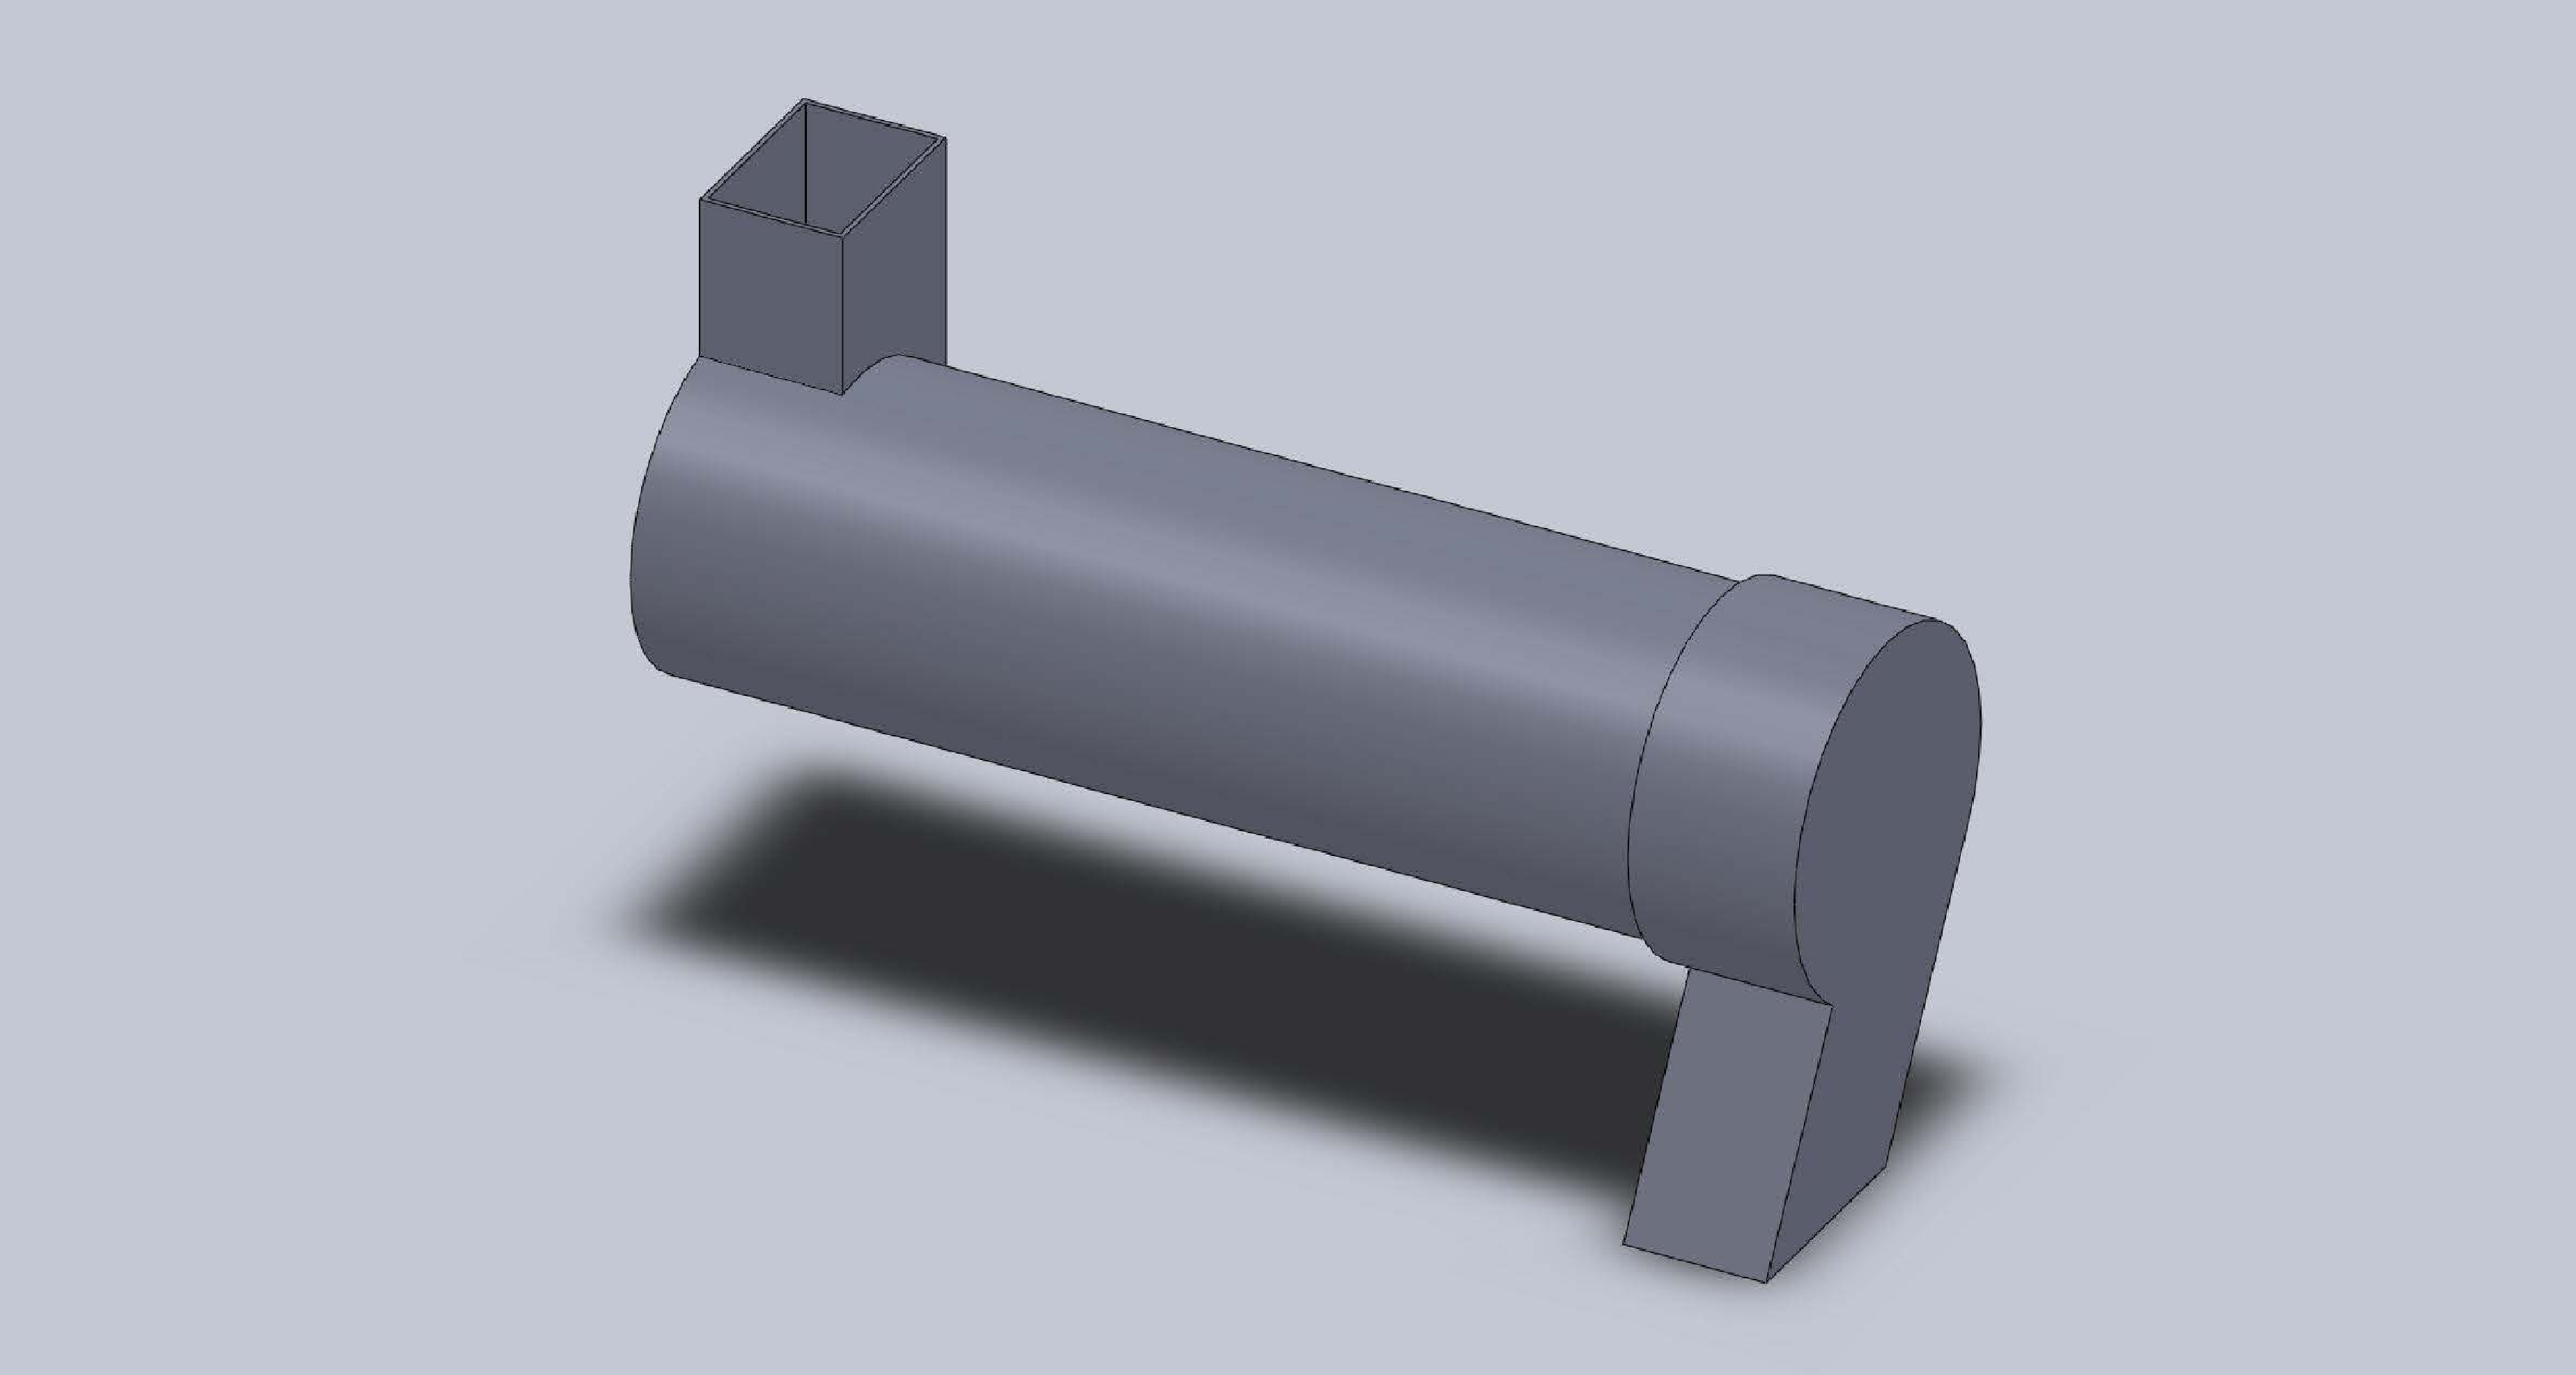
\includegraphics[scale=0.15]{shell_final_pic.pdf}
\caption{The isometric view of the L\"{o}dige CoriMix CM5 continuous high shear granulator casing.}
\label{fig:mthdsDemCharlesGranShell}
\end{figure}

The impeller consists of a cylindrical shaft of length 370 mm and diameter 68 mm with four 
flattened sides 15 mm wide running along the axis. The blades are placed on these flattened sides as 
shown in Figure~\ref{fig:mthds_dem_charles_impeller}. There are three different blade elements on the 
shaft (Figure~\ref{fig:mthds_dem_charles_fig5pt3and4_blades_n_isometric}). At the granulator inlet, 
there are 4 paddle shaped feed elements following which there are 20 tear drop shaped shearing 
elements  and finally 4 trapezoidal blades near the exit. All these elements are placed in 
a spiral configuration. 

\begin{figure}
\centering
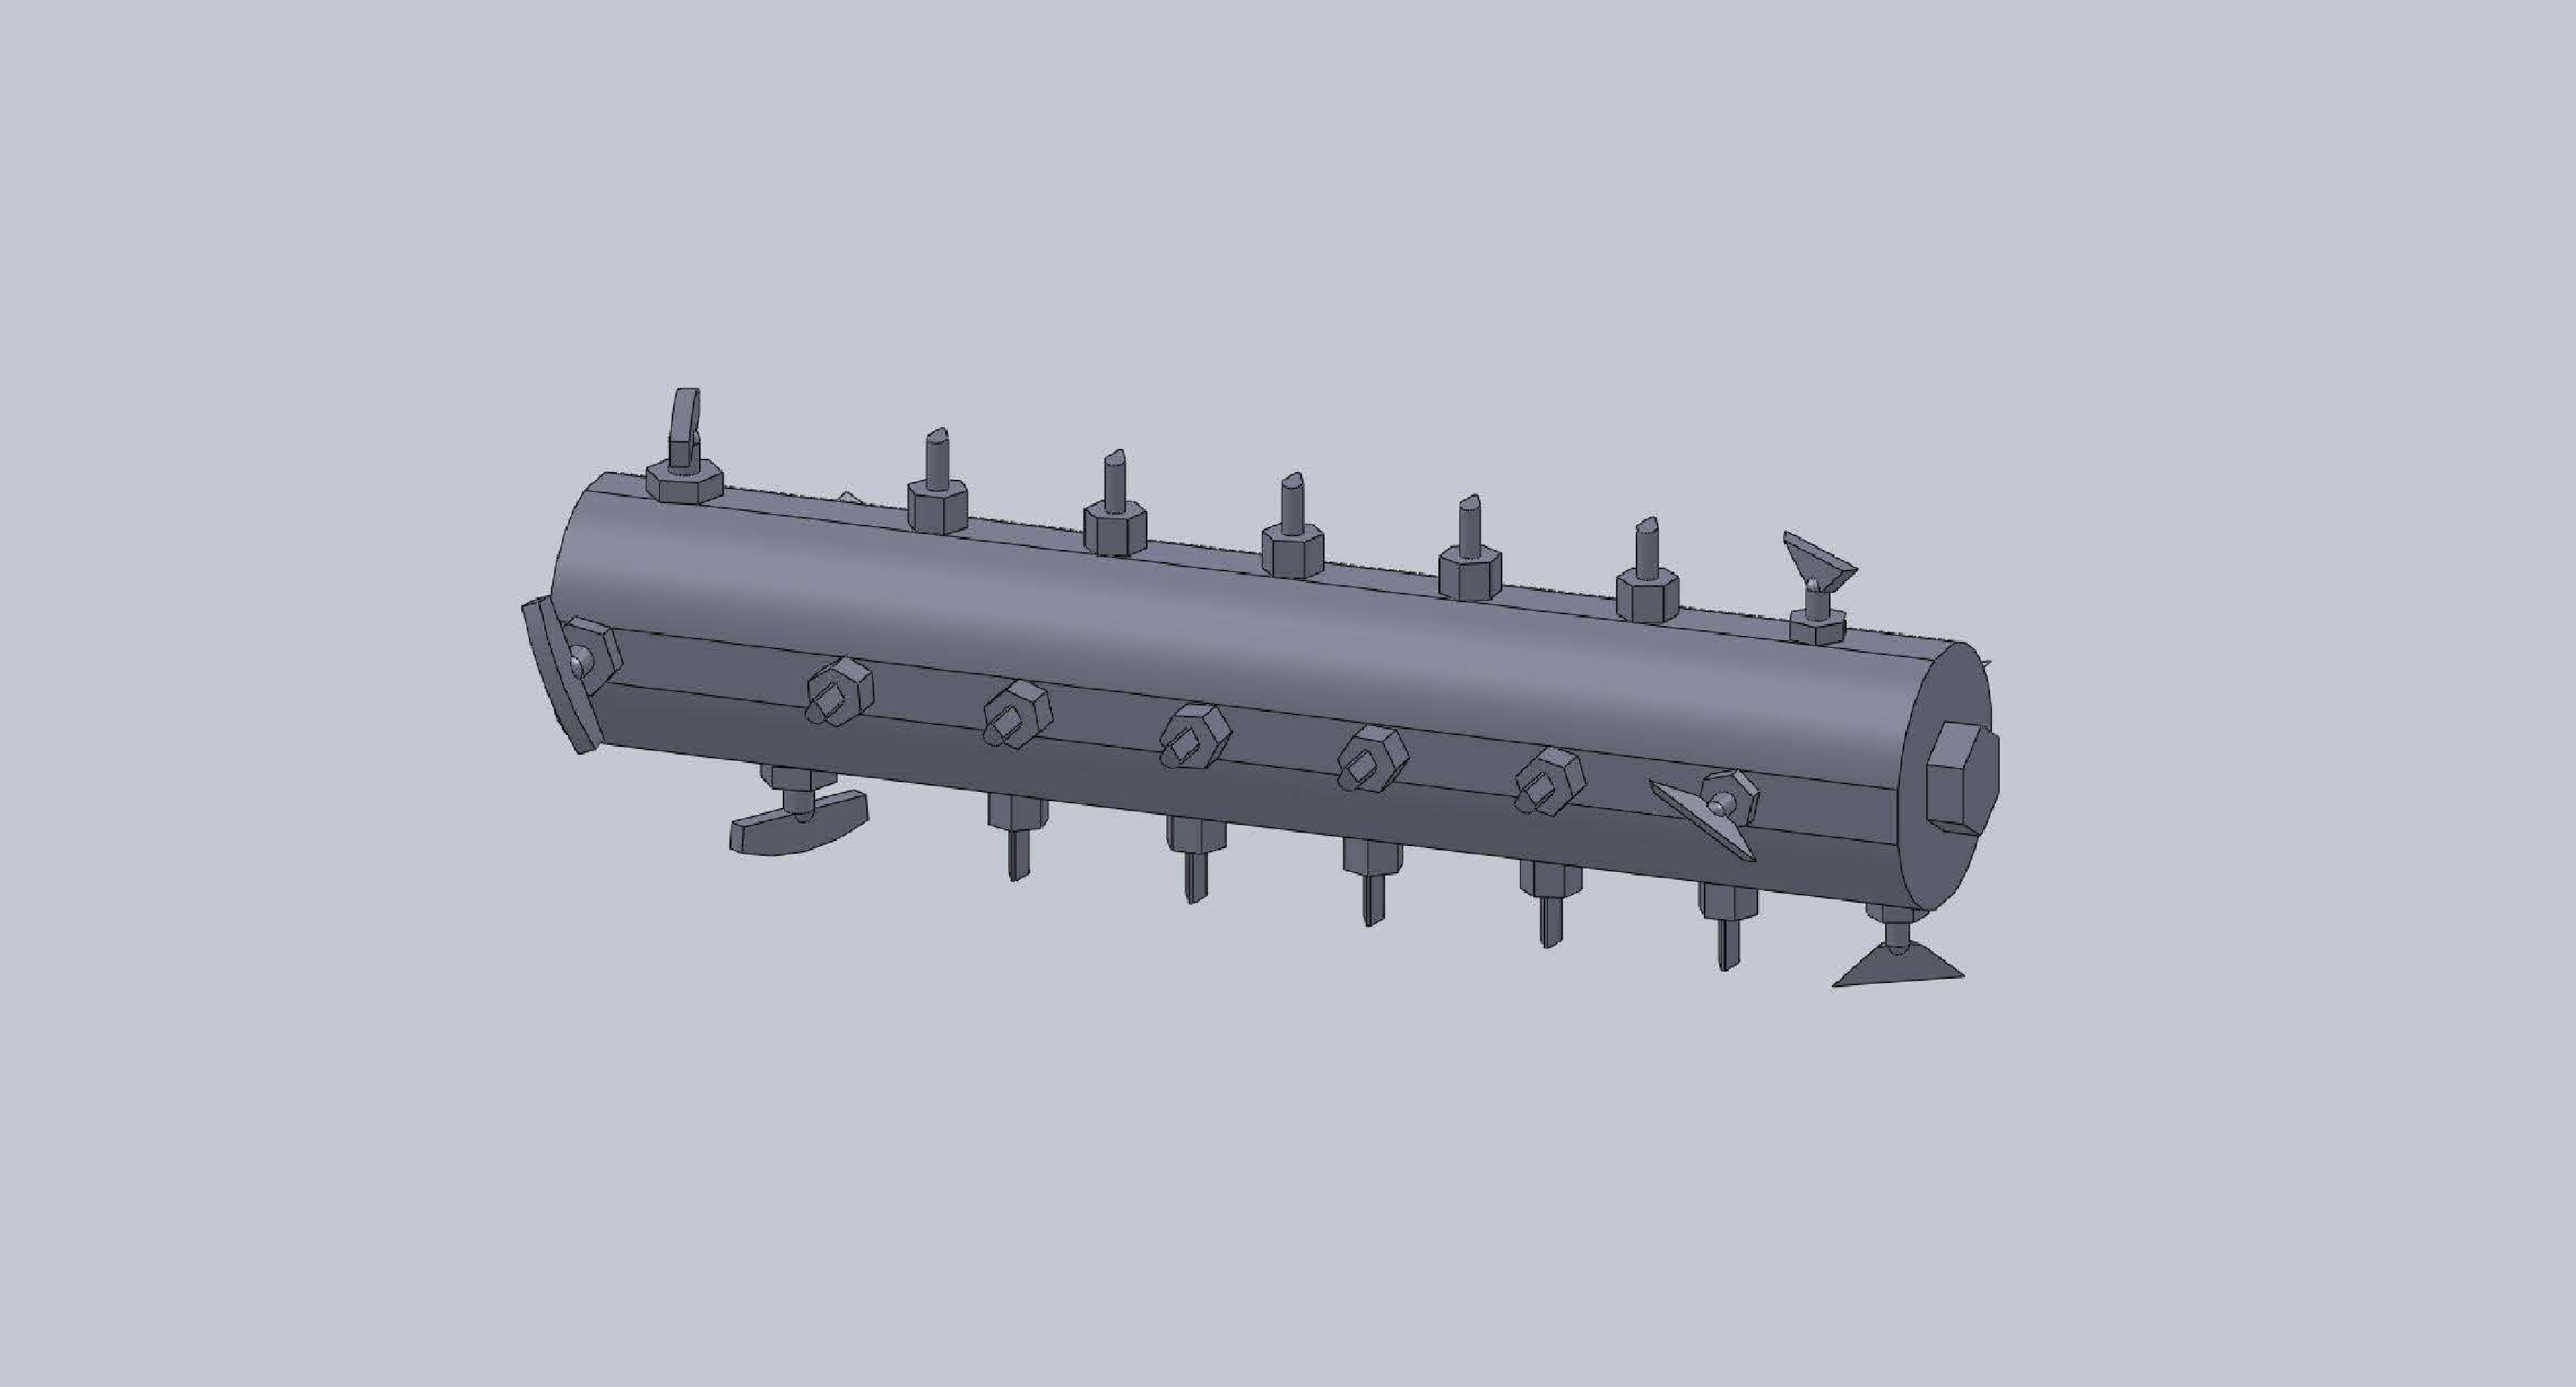
\includegraphics[scale=0.15]{impeller_final_pic.pdf}
\caption{This shows the isometric view of the impeller inside the L\"{o}dige CoriMix CM5 continuous 
high shear granulator casing.}
\label{fig:mthds_dem_charles_impeller}
\end{figure}    

\begin{figure}
\begin{subfigure}{.3\textwidth}
\centering
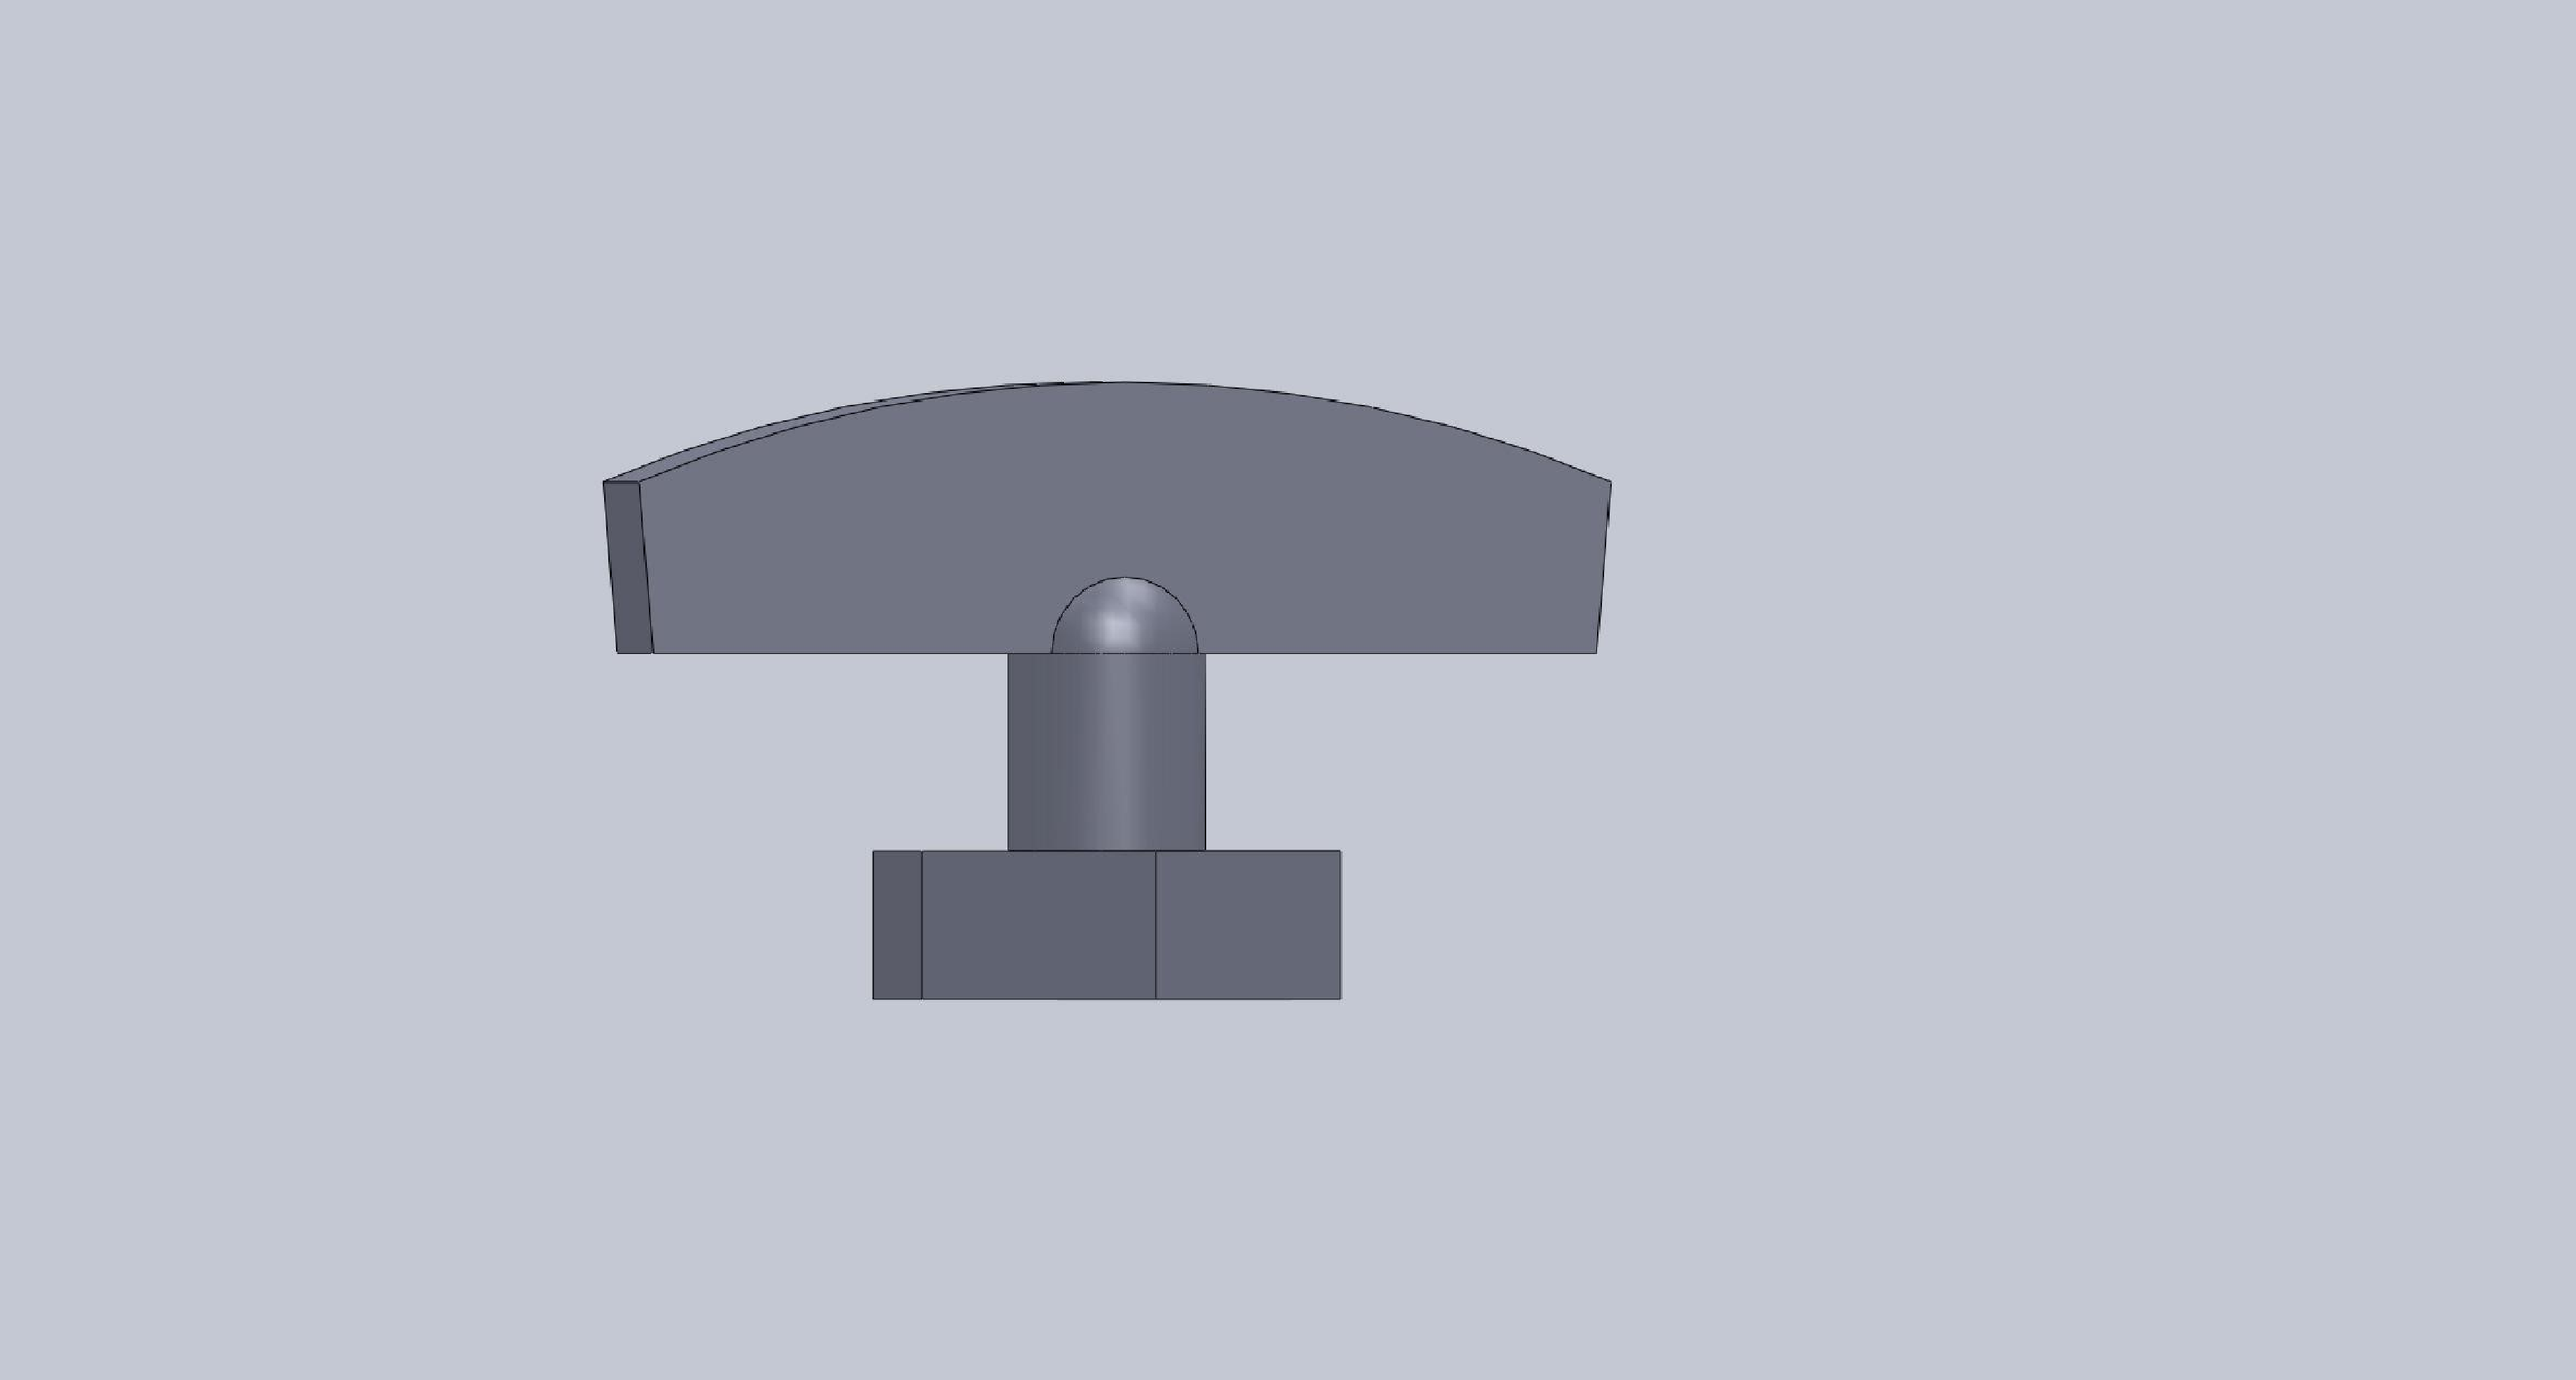
\includegraphics[scale=0.075]{feed_element.pdf}	      
\caption{Feed element}
\label{fig:mthds_dem_feed_element}
\end{subfigure}%
\begin{subfigure}{.3\textwidth}
	\centering
	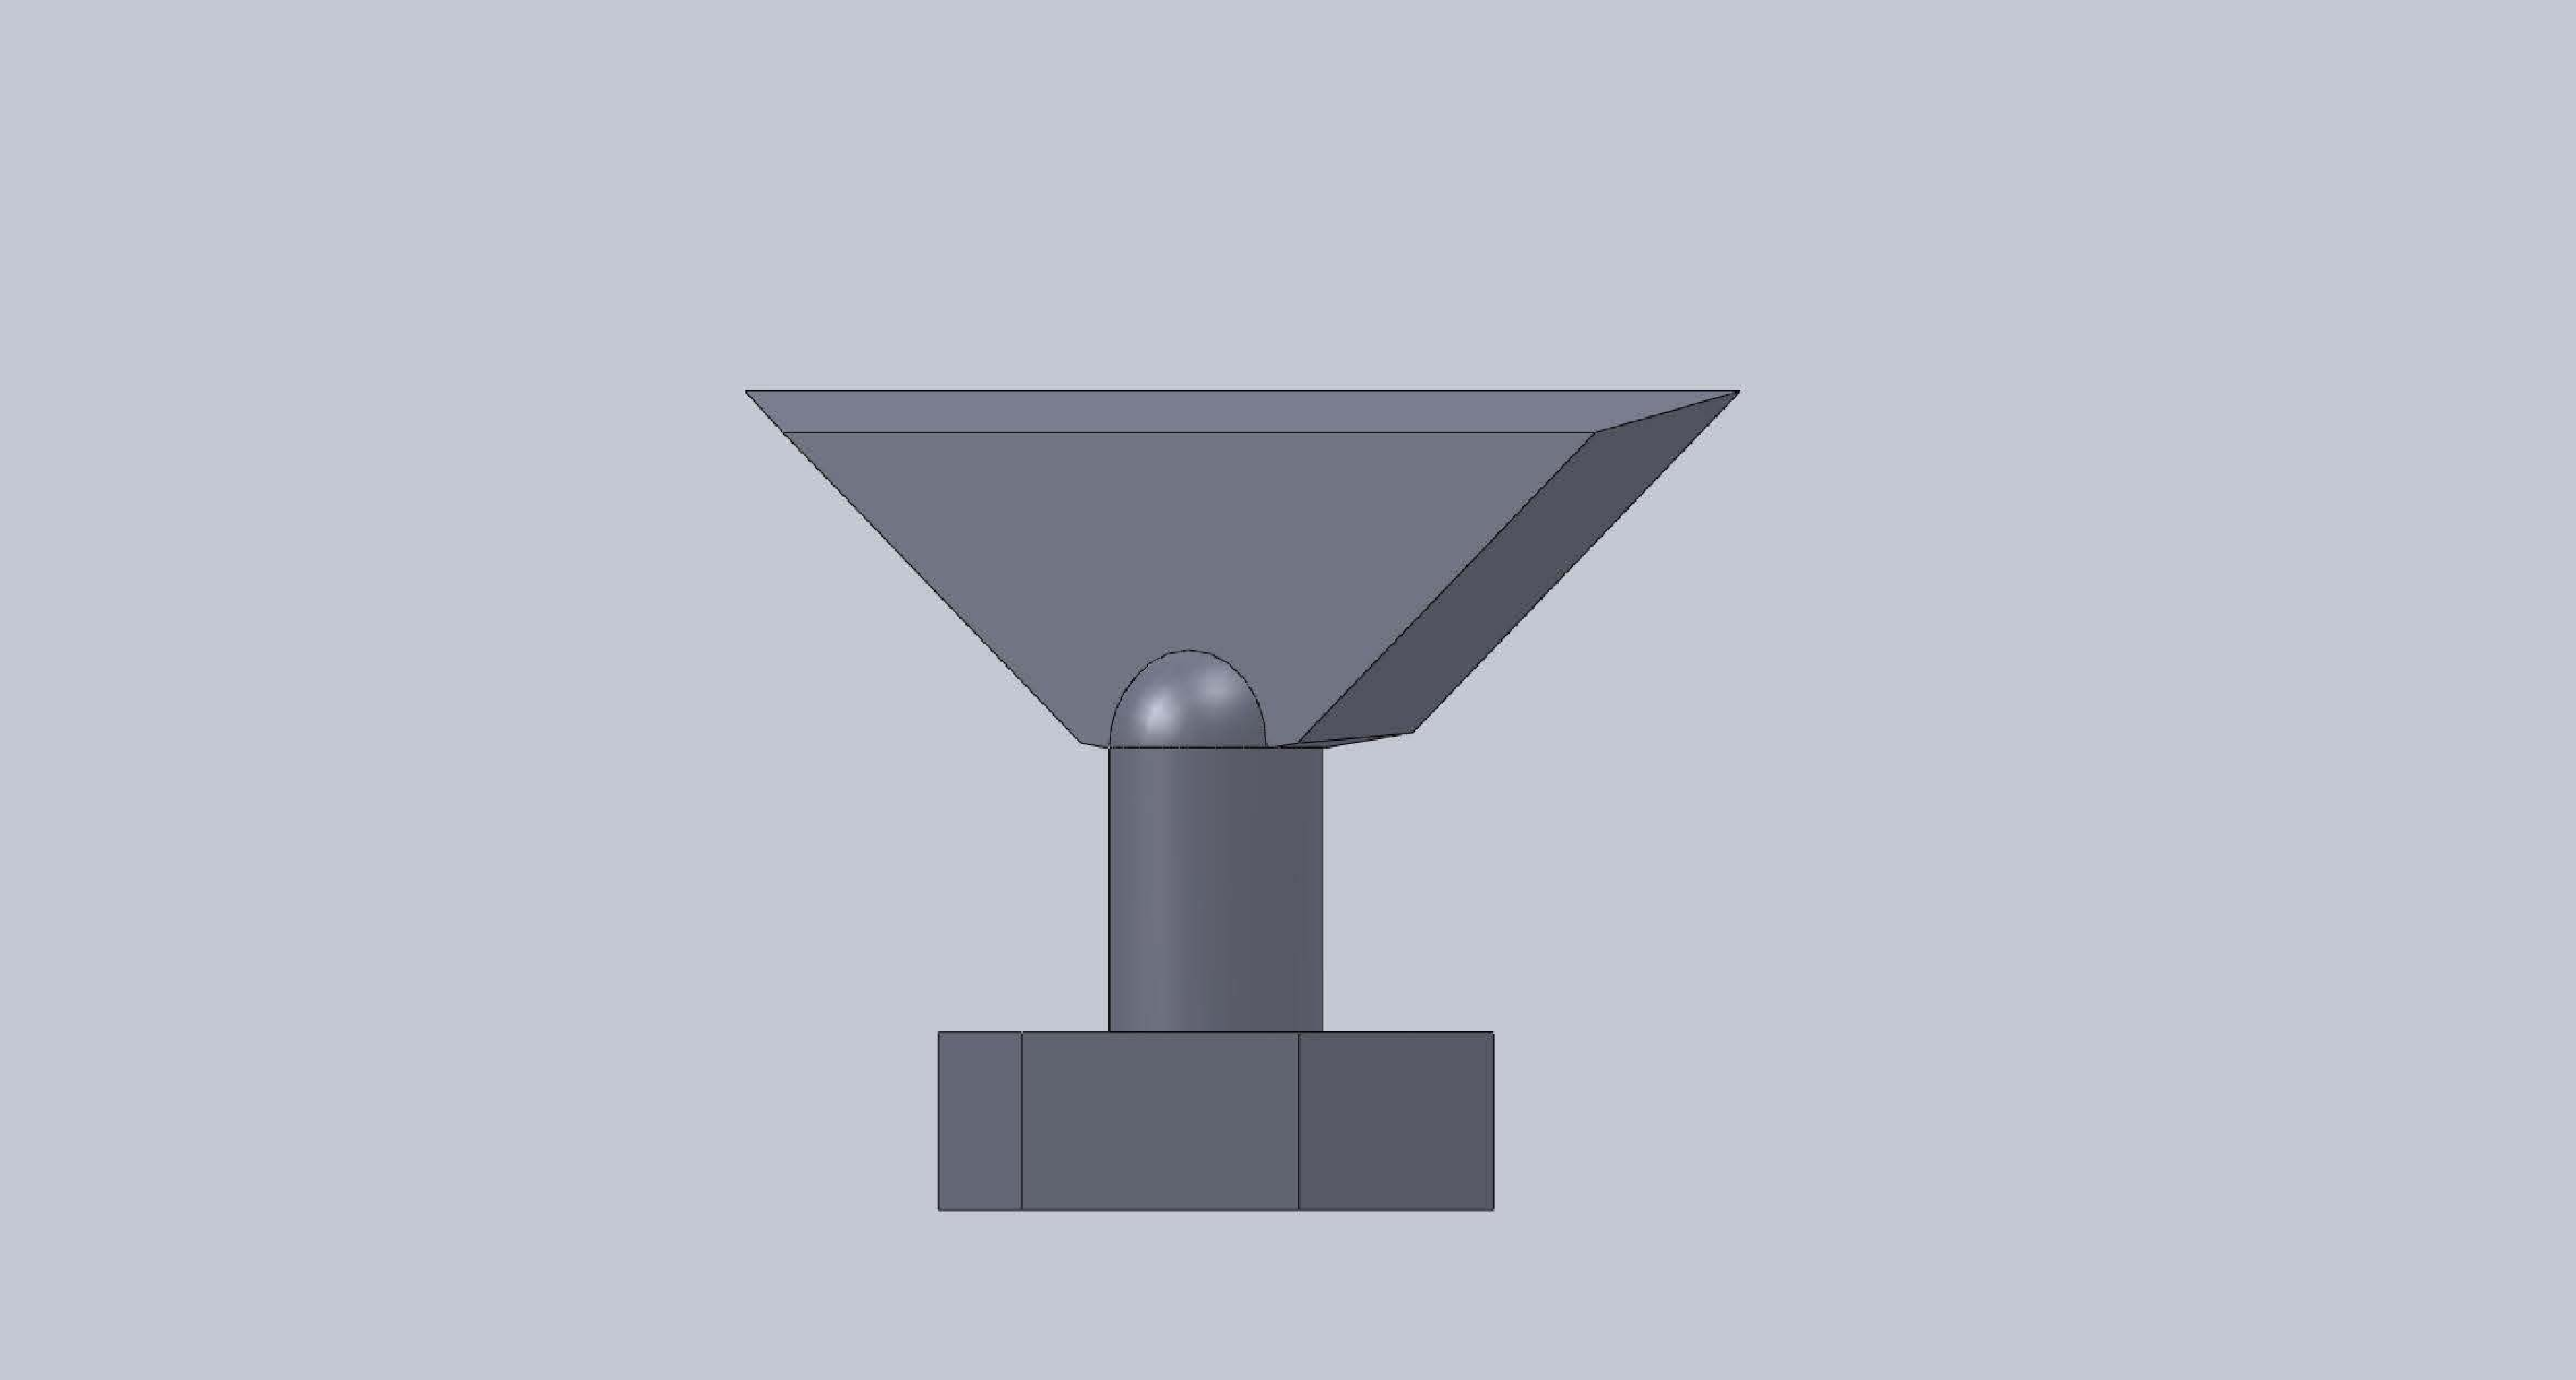
\includegraphics[scale=0.075]{exit_element.pdf}
	\caption{Exit element}
	\label{fig:mthds_dem_exit_element}
\end{subfigure}
\begin{subfigure}{.3\textwidth}
\centering
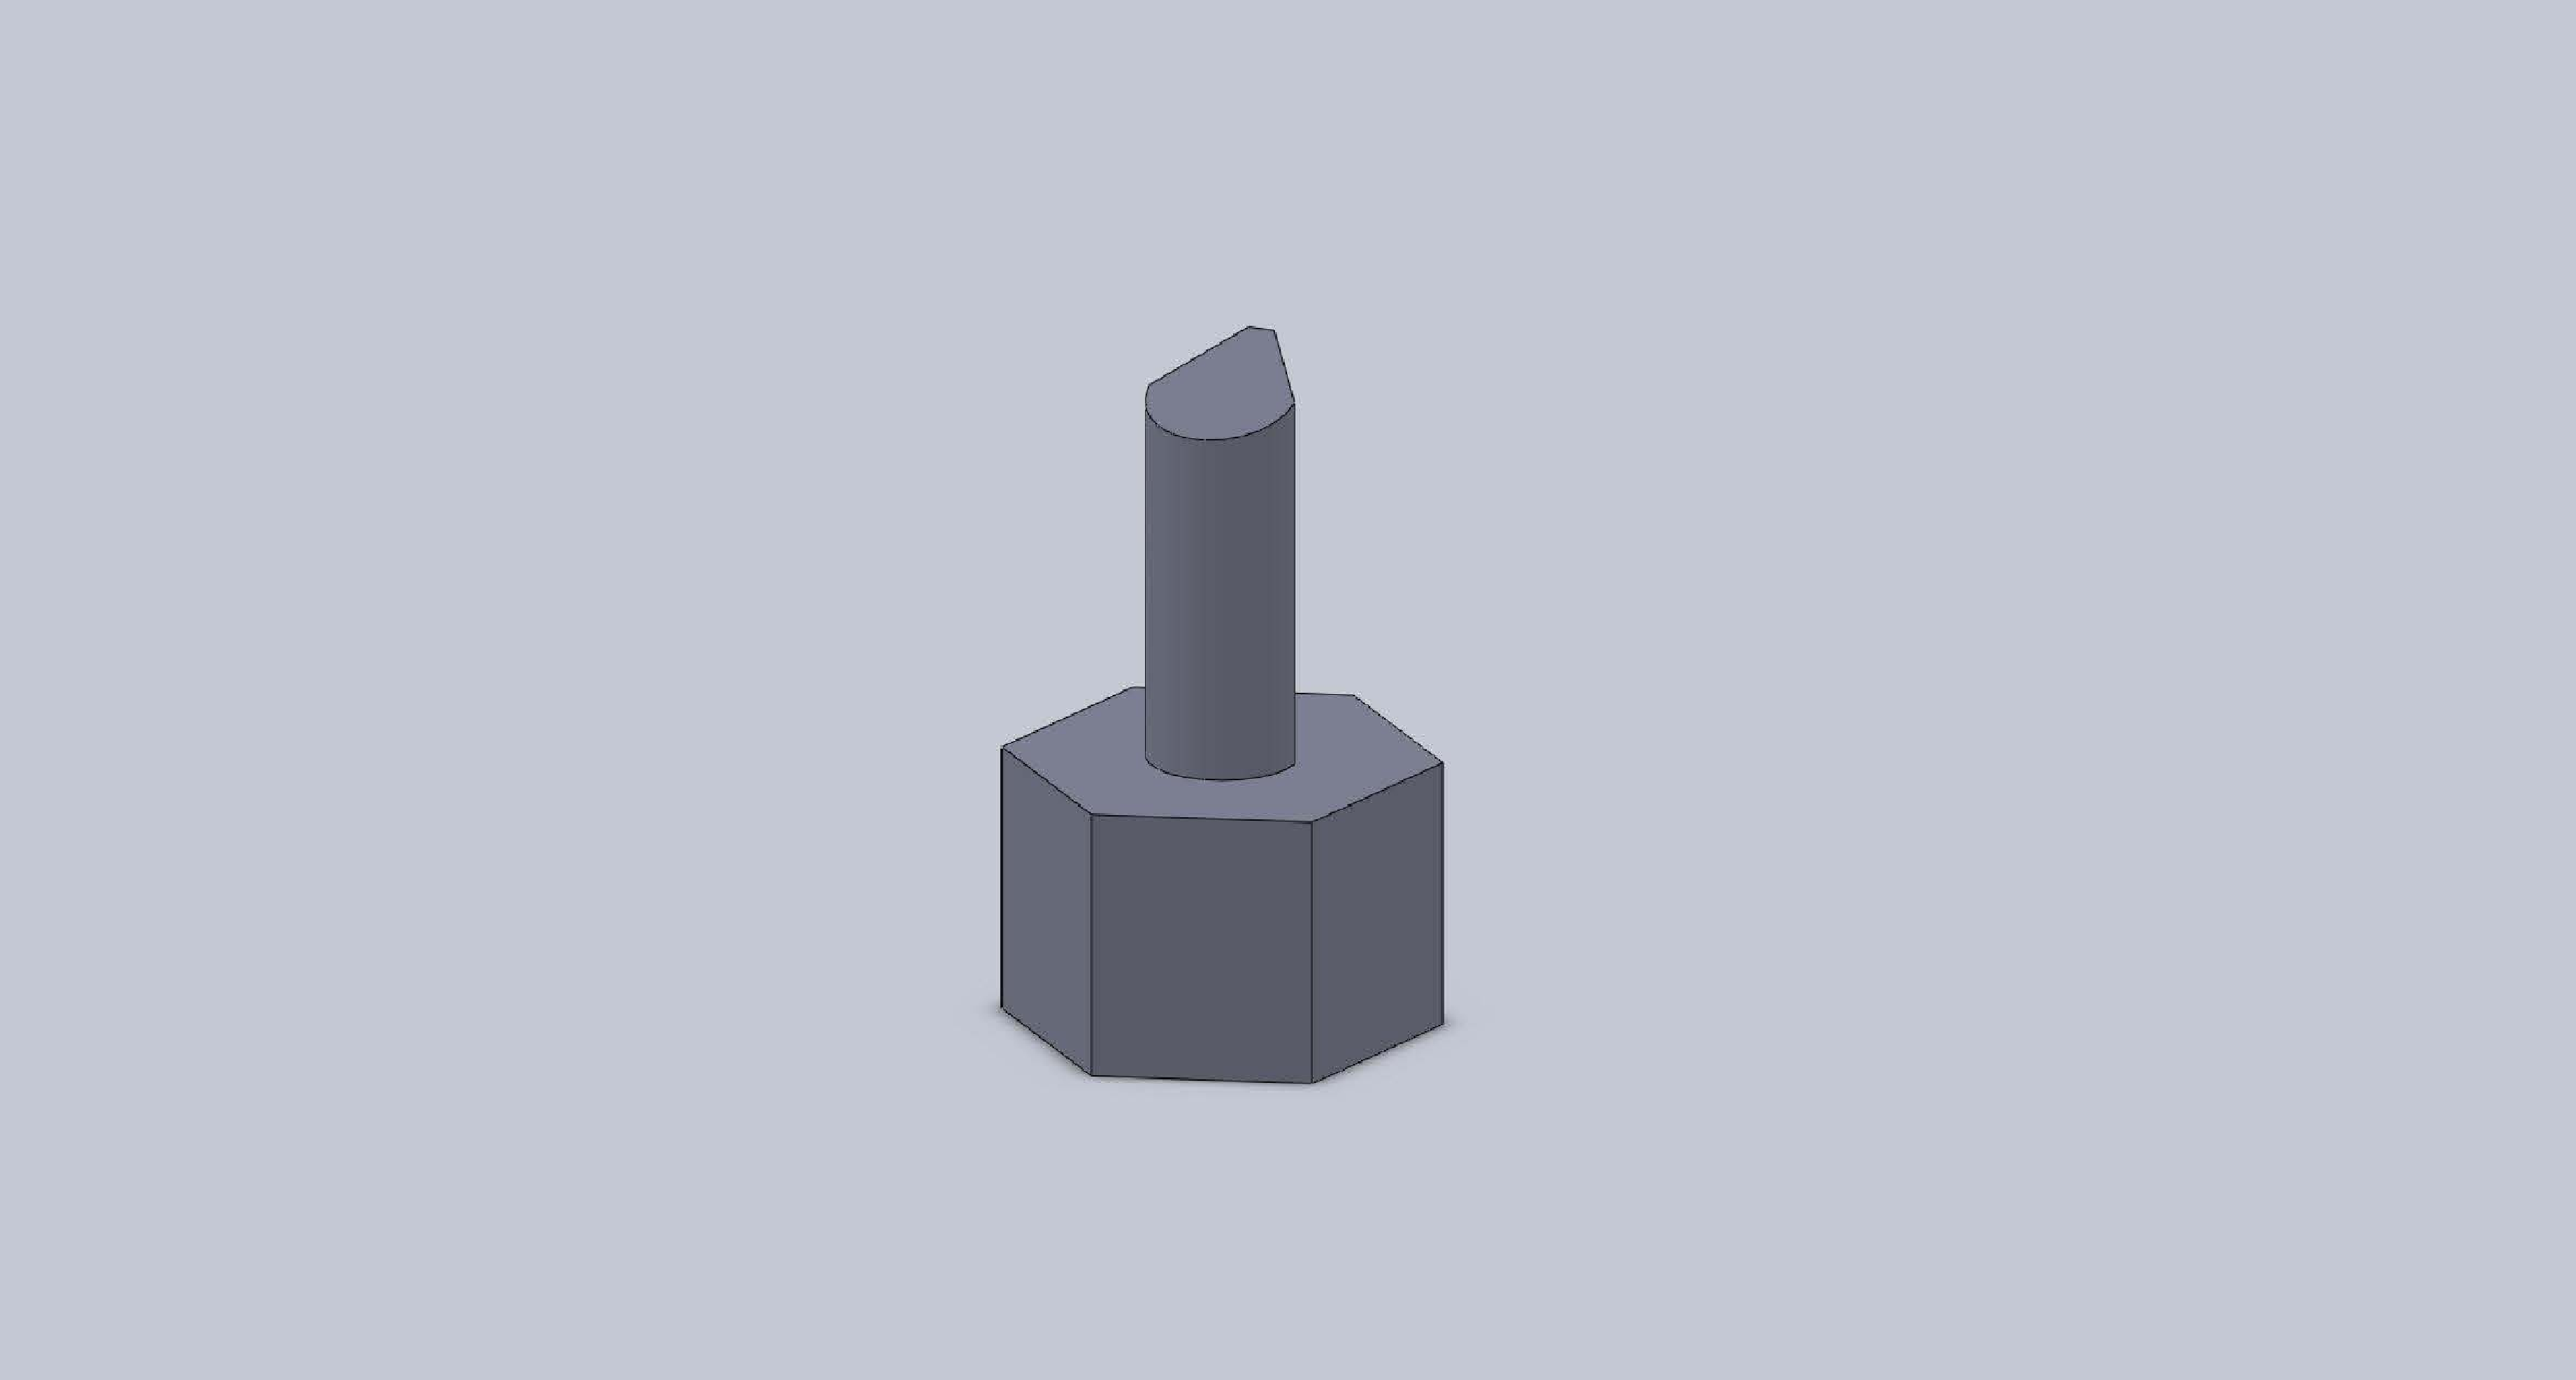
\includegraphics[scale=0.075]{shear_element.pdf}
\caption{Shear element}
\label{fig:mthds_dem_shear_element}
\end{subfigure}
\caption{Components (\subref{fig:mthds_dem_feed_element}) and (\subref{fig:mthds_dem_exit_element}) help in the forward 
movement of the particles while (\subref{fig:mthds_dem_shear_element}) aids to direct the particles to the wall 
inside the L\"{o}dige CoriMix CM5 continuous high shear granulator.}
\label{fig:mthds_dem_charles_fig5pt3and4_blades_n_isometric}
\end{figure}     

After the geometry was built in SolidWorks$^{TM}$ (Dassault Syst\`{e}mes) the shell and impeller 
were exported as stereo-lithography (STL) files. The coarsest output option was used to keep the 
STL files small for faster computation times. The origin of the geometry was not preserved 
while saving the STL files since it needs to be aligned in LIGGGHTS as per the process conditions. 
Meshlab was used to align the STL files for importing. No mesh treatments were used on the STLs. 
The meshes were then imported into LIGGGHTS using the write command in serial. 
The write exclusion list command was used and this exclusion list file is then used in the 
simulation to skip the highly skewed elements during the simulation. 


\subsubsection{DEM Software and Input Setup}
LIGGGHTS v3.60 developed by DCS computing was used for all the DEM simulations 
performed in this study. Source code files were modified to obtain particle-particle 
collisions. This version of LIGGGHTS was compiled using the mvapich (mvapich2 v2.1) 
and intel (intel v15.0.2) compilers with the -O3 optimization option as well as an 
option to side load the process to the Xeon phi co-processors was added. The 
initial timing studies were performed on Stampede supercomputer located at TACC, 
University of Texas, Austin. The hardware configuration of each node consists 
of 2 8-core Intel Xeon E5-2680 processors based on the Sandy Bridge architecture, 
32 GB of memory with QPI interconnects.

The DEM simulation in LIGGGHTS are setup using an input script which defines physical 
parameters of the particles, importing of the geometry, particle insertion commands, various physics 
models to be used during the simulation as well as various compute and dump commands to help print 
data required for post-processing. The particles were considered to be granular in 
nature. The Hertz-Mindlin model was used for non-adhesive elastic contact between 
the granular particles. 
Particles were inserted inside the granulator from the inlet at a constant mass flow rate of 15 
kilograms per hour. Rotation speed of the impeller was kept throughout the study at 2000 rotations 
per minute. Such a high rotation speed was chosen since this would lead to high shear between the 
particles and walls of the shell resulting in better size control of the granules. 
There were two sets of 
simulations that were performed, one with mono-sized particles and second consisting 
of a distribution 
of sizes. The particle radii chosen for mono-sized simulation varied from 0.59mm to 2mm, consecutive 
particles radii had twice the volume of particles before them. The radii range of the distributed 
size simulation was 1mm to 3mm. The difference in mechanics of these two simulations is discussed 
in the Section~\ref{sec:Results}. Physical constants used for the simulations are given in 
Table~\ref{table:mthds_dem_input}.

The simulation data was collected after every 50,000 time steps (5$\times 10^{-3}$ sec) 
for the visualization of the particles inside the shell, further post processing . The collisions 
between each of the particles and collisions between particle and the geometry was 
collected and used in the PBM. 

\begin{table}
\caption{Physical Properties of the particle for the LIGGGHTS input script} 
\label{table:mthds_dem_input}
\begin{center}
\begin{tabular}{l|c|c}
\hline
\bf{Parameter} &\bf{Value} &\bf{Units}\\
\hline
Young's Modulus of particles  & $8 \times 10^{6}$ & $N.m^{-2}$\\
Young's Modulus of Geometry  & $1 \times 10^{9}$ & $N.m^{-2}$\\
Poisson's Ratio & $0.2$ & $-$\\
Coefficient of restitution (constant for all collisions) & $0.4$ & $-$\\
Coefficient of static friction & $0.5$ & $-$\\
Coefficient of rolling friction  & $0.2$ & $-$\\
Density of the granules & $500$ & $kg.m^{-3}$\\
\hline
\end{tabular}
\end{center}
\end{table}

\subsubsection{Population Balance Modeling (PBM) development}
\label{sec:pbm_model}
 The population balance equation used in this work is expressed below:
\begin{align}
\frac{d}{dt}F(s_1,s_2,x,t)=\Re_{agg}(s_1,s_2,x,t)+\Re_{break}(s_1,s_2,x,t)+
\dot{F}_{in}(s_1,s_2,x,t)-\dot{F}_{out}(s_1,s_2,x,t)
\label{eqn:mthds_pbm_overall} 
\end{align}
where, $F(s_1,s_2,x)$ is the number of particles with an active pharmaceutical ingredients 
(API) volume of $s_1$ and an excipient 
volume of $s_2$ in the spatial compartment $x$. The rate of change of number of particles with time 
in different size classes depend on the rate of aggregation $\Re_{agg}(s_1,s_2,x,t)$ and the rate of 
breakage $\Re_{break}(s_1,s_2,x,t)$. Also, the rate of particles coming into, $\dot{F}_{in}(s_1,s_2,x,t)$ and 
going out, $\dot{F}_{out}(s_1,s_2,x,t)$ of the spatial compartment due to particle transfer affect the 
number of particles in different size classes. 
The rate of change of liquid volume for a given time in each particle is calculated using the equation: 

\begin{align}
\frac{d}{dt}F(s_1,s_2,x,t)l(s_1,s_2,x,t)&= 
\Re_{liq,agg}(s_1,s_2,x,t)+\Re_{liq,break}(s_1,s_2,x,t)+\dot{F}_{in}(s_1,s_2,x,t)l_{in}(s_1,s_2,x,t)\notag\\
&-\dot{F}_{out}(s_1,s_2,x,t)l_{out}(s_1,s_2,x,t)+F(s_1,s_2,x,t)\dot{l}_{add}(s_1,s_2,x,t)
\label{eqn:mthds_pbm_rate} 
\end{align}

where, $l(s_1,s_2,x,t)$ is the amount of liquid volume in each particle with API volume of $s_1$ and 
excipient volume of $s_2$ in the spatial compartment $x$. $\Re_{liq,agg}(s_1,s_2,x,t)$ and 
$\Re_{liq,break}(s_1,s_2,x,t)$ are respectively the rates of liquid transferred between size classes due to 
aggregation and breakage. $l_{in}(s_1,s_2,x,t)$ and $l_{out}(s_1,s_2,x,t)$ are respectively the liquid 
volumes of the particles coming in and going out of the spatial compartment.~$\dot{l}_{add}(s_1,s_2,x,t)$ is 
the volume of liquid acquired by each particle in the compartment at every time step due to external 
liquid addition.
Similarly, the rate of change of gas volume for a given time is calculated using the following equation: 

\begin{align}
\frac{d}{dt}F(s_1,s_2,x,t)g(s_1,s_2,x,t)&= 
\Re_{gas,agg}(s_1,s_2,x,t)+\Re_{gas,break}(s_1,s_2,x,t)+\dot{F}_{in}(s_1,s_2,x,t)g_{in}(s_1,s_2,x,t)\notag\\
&-\dot{F}_{out}(s_1,s_2,x,t)g_{out}(s_1,s_2,x,t)+F(s_1,s_2,x,t)\dot{g}_{cons}(s_1,s_2,x,t)
\label{eqn:mthds_pbm_gas_agg} 
\end{align}

where, $g(s_1,s_2,x,t)$ is the gas volume of each particle with API volume of $s_1$ and excipient 
volume of $s_2$ in the spatial compartment $x$. $\Re_{gas,agg}(s_1,s_2,x,t)$ and 
$\Re_{gas,break}(s_1,s_2,x,t)$ are respectively the rates of gas transferred between size classes due to 
aggregation and breakage. $g_{in}(s_1,s_2,x,t)$ and $g_{out}(s_1,s_2,x,t)$ are respectively the gas 
volume of the particles entering and leaving the spatial compartment. $\dot{g}_{cons}(s_1,s_2,x,t)$ is the 
volume of gas coming out of each particle at every time-step due to consolidation of the particles. 
The rate of aggregation, $\Re_{agg}(s_1,s_2,x,t)$ in Equation~\ref{eqn:mthds_pbm_overall} is 
calculated as~\citep{Chaturbedi2017}:

\begin{align}
\Re_{agg}(s_1,s_2,x,t)&= \frac{1}{2}\int _0^{s_1} \int_0^{s_2} 
\beta(s_1',s_2',s_1-s_1',s_2-s_2',x,t)F(s_1',s_2',x,t)F(s_1-s_1',s_2-s_2',x,t)ds_1'ds_2'\notag\\ 
&- F(s_1,s_2,x,t)\int _0^{s_{max_1}-s_1} \int_0^{s_{max_2}-s_2} 
\beta(s_1,s_2,s_1',s_2',x,t)F(s_1',s_2',x,t)ds_1'ds_2'
\end{align}


where, $s_1'$ \& $s_2'$ represent for 2 different particles inside the powder granule. 
The aggregation kernel $\beta(s_1,s_2, s_1',s_2',x)$ is expressed as a function of the collision 
rate coefficient ($C$) and probability that a collision will result in agglomeration($\psi$)
~\citep{ingram2004} and is shown below: 

\begin{align}
\beta(s_1,s_2,s_1',s_2',x) = \beta_oC(s_1,s_2,s_1',s_2',x)\psi(s_1,s_2,s_1',s_2',x)
%\beta(s_1,s_2,s_1',s_2',x) = & \beta_o*(V(s_1,s_2,x)+V(s_1',s_2',x))^{\gamma}*(c(s_1,s_2,x)\notag\\
%&+c(s_1',s_2',x))^{\alpha}\left(1-\frac{(c(s_1,s_2,x)+c(s_1',s_2',x))^{\delta}}{2}\right)^{\alpha}
\label{eqn:mthds_pbm_beta_kernal}
\end{align}

where, $\beta_o$ is aggregation rate constant.\\
Collision rate coefficient ($C$) is a function of particle sizes and is calculated by normalizing the 
number of collisions between a group of particles~\citep{gantt2006} and is obtained from a LIGGGHTS 
DEM simulation. Collision rate coefficient for every time step can be expressed as:

\begin{align}
C(s_1,s_2,s_1',s_2')=\frac{N_{coll}(s_1,s_2,s_1',s_2')}{N_p(s_1,s_2)N_p(s_1',s_2')\Delta t}
\label{eqn:collfreq}
\end{align}

In Equation~\ref{eqn:collfreq}, $N_{coll}$ is the number of collisions between two particles in 
time interval $\Delta t$ and $N_p$ is the number of particles of a particular size. The agglomeration 
($\psi$) in Equation~\ref{eqn:mthds_pbm_beta_kernal} can be expressed as:

\begin{align}
\psi((s_1,s_2,s_1',s_2') = 
\left\{\begin{matrix}
\psi_0,\hspace{0.2cm} LC((s_1,s_2) \geq LC_{min}\hspace{0.2cm} and\hspace{0.2cm} LC((s_1',s_2') \geq LC_{min}	\\ 
0,\hspace{0.2cm} LC((s_1,s_2) < LC_{min}\hspace{0.2cm} or\hspace{0.2cm} LC((s_1',s_2') < LC_{min}
\end{matrix}\right.
\label{eqn:colleff}
\end{align}
 In Equation~\ref{eqn:colleff}, $LC$ is the liquid content of particles and $LC_{min}$ stands for minimum 
 liquid content required for coalescence of particles. 

The rate of increase of liquid volume of a particle, $\dot{l}_{add}(s_1,s_2,x)$ is expressed as:

\begin{align}
\dot{l}_{add}(s_1,s_2,x) = \frac{(s_1+s_2)(\dot{m}_{spray}(1-c_{binder})-\dot{m}_{evap})}{m_{solid}(x)}
\end{align}

where, $(s_1+s_2)$  is the total solid volume of the particle; $\dot{m}_{spray}$ is the rate of external 
liquid addition, $c_{binder}$ is the concentration of binder in the external liquid (which is assumed to 
be zero in this case); $\dot{m}_{evap}$ is the rate of evaporation of liquid from 
the system (which is also assumed to be zero in this case) and $m_{solid}$ is the total amount of solid 
present in the compartment.
The rate of decrease in gas volume per particle due to consolidation is calculated using the 
following expression:~\citep{Verkoeijen2002} 

\begin{align}
\dot{g}_{cons}(s_1,s_2,x,t)=& c \nu_{impeller}^{\omega}V(s_1,s_2,x)\frac{(1-\epsilon_{min})}{s} 
\notag \\ 
& \left[g(s_1,s_2,x,t)+l(s_1,s_2,x,t) -(s_1+s_2)\frac{\epsilon_{min}}{1-\epsilon_{min}}\right]
\end{align}        

 where, $c$ and $\omega$ are the consolidation constants; $v_{impeller}$ is the impeller 
rotational speed; $V(s_1,s_2,x)$ is the volume of particle, $\epsilon_{min}$ is the minimum porosity; 
$g(s_1,s_2,x)$ and $l(s_1,s_2,x)$ are respectively the gas and liquid volumes of the particle.

Particle transfer rate, $\dot{F}_{out}(s_1,s_2,x)$ in Equation~\ref{eqn:mthds_pbm_overall} is calculated 
as:

\begin{align}
\dot{F}_{out}(s_1,s_2,x) = \dot{F}(s_1,s_2,x)\frac{\nu_{compartment}(x)*dt}{d_{compartment}}
\end{align}

where, $\nu_{compartment}(x)$ and $d_{compartment}$ are respectively the average velocity of 
particles in compartment $x$ and the distance between the mid-points of two adjacent compartment, 
which is the distance particles have to travel to move to the next spatial compartment. $dt$ is the 
time-step.
The process parameters and physical constants used in the PBM simulation are listed in Table~\ref{table:mthds_pbm_parameters}.
\begin{table}
\caption{Parameters used in the PBM simulation}
\label{table:mthds_pbm_parameters}
\begin{center}
\begin{tabular}{l|c|c|c}
\hline
\bf{Parameter} &\bf{Symbol} &\bf{Value} &\bf{Units}\\
\hline
Initial time step & $\delta t$ & $0.5$ & $s$\\
Mixing time & $T$ & $25$ & $s$\\
Granulation time & $T$ & $75$ & $s$\\
Velocity in axial direction & $v_{axial}$ & $1$ & $ms^{-1}$\\
Velocity in radial direction & $v_{radial}$ & $1$ & $ms^{-1}$\\
Aggregation constant & $\beta_0$ & $1\times10^{-9}$ & $-$\\
Initial particle diameter & $R$ & $150$ & $\mu m$\\
%Breakage kernel constant & $B$ & $0$ & $-$\\
Diameter of impeller & $D$ & $0.114$ & $m$ \\
Impeller rotation speed & $RPM$ & $2000$ & $rpm$\\
Minimum granule porosity & $\epsilon_{min}$ & $0.2$ & $-$\\
Consolidation rate & $C$ & $0$ & $-$\\
Total starting particles in batch & $F_{initial}$ & $1 \times 10^{6}$ & $-$\\
Liquid to solid ratio & $L/S$ & $0.35$ & $-$ \\
Number of Compartments & $c$ & $16$ & $-$ \\
Number of first solid bins & $s$ & $16$ & $-$\\
Number of second solid bins & $ss$ & $16$ & $-$\\
\hline
\end{tabular}
\end{center}
\end{table}

\subsection{Development and Experiment Analysis}
\subsubsection{DEM post processing}
Post processing of data obtained from the DEM simulations was done using MATLAB. 
The first test run on the output data was to determine if the simulation had reached steady-state. The 
mass inside the granulator was found out by averaging it over 5 time steps and then compared to 
mass inside the granulator after every 10000 time steps (about 5$\times 10^{-4}$ sec) with a 
tolerance of 10\%. If the mass was found to be constant for most of the iterations, it was 
considered to be at steady state. Another test to determine steady state was to monitor the number of 
collision inside the granulator. The visualization of the simulation data was done by running the 
LIGGGHTS post processing (LPP) script over the dump files to convert them into STL files. These 
files were then loaded in to Paraview~\citep{paraview2017} for a graphical 
representation of the 
simulation. It can be seen that the number of collision start to oscillate around a mean value. The 
number of collisions were then plotted and steady state time was determined.
A precautionary script was also run so as to determine that no particles were lost due to overlap 
of the geometry with the particles as well as from particle-particle overlap.


\subsubsection{Parallel PBM approach}
The PBM was discretized by converting each of its coordinates in to discrete
bins. For the spatial coordinates a linear bin spacing was used. For the
internal coordinates, solid, liquid, and gas a non-linear discretization was
used~\citep{barrasso2012}. Once the PBM had been discretized, a finite
differences method was used which created a system of ordinary differential
equations (ODEs)~\citep{Barrasso2015cerd}. The numerical integration technique
used to evaluate the system of ODEs was first order Euler integration as it is
commonly used to solve these types of systems and ~\citep{Barrasso2013} 
found it decreased computation time while having minimal impact on 
accuracy as opposed to other integration techniques. In
order to avoid numerical instability due to the explicit nature of the Euler
integration, Courant-Friedrichs-Lewis (CFL) condition must be
satisfied~\citep{courant1967}. For the PBM model, a time-step was calculated at
each iteration such that, the number of particles leaving a particular bin at
any time was less than the number of particles present at that
time~\citep{Ramachandran2010}.

The model was parallelized such that it
could take advantage of shared memory but still effectively run across a
distributed system, thus employing a combination of both, MPI and OMP.

An algorithm in the form of pseudo code is presented in Algorithm \ref{alg:parallelPBM} illustrating how
the calculations are distributed and carried out during the simulation. For
each time step, the MPI processes are made responsible for a specific chunk of
the spatial compartments. \\
\jhanote{please use proper format to present an
algorithm. giannis please use format of CCGrid paper, for example} \csnote{re-wrote the algorithm please 
have a look}
\gpnote{Yes, it is in the same format as the CCGrid paper. Much better than before. I suggest that you 
reference the algorithm. Using "below" I expect the algorithm near this paragraph, but it is in the Appendix.}
\csnote{Have added it back to this section}\\
 Then each OMP thread, inside of each MPI process, is allocated to one of the cores of
multi-core CPU the MPI process is bound too. The OMP threads divide up and
compute $\Re_{agg}$. After $\Re_{agg}$ is calculated the MPI processes
calculate the new PSD value ($F_{t,c}$) for their chunk at that specific time step
. The slave processes send their $F_{t,c}$ to the master processes
which collects them into the complete PSD ($F_{t,all}$). The master process then
broadcasts the $F_{t,all}$ value to all slave processes. This decomposition of
the data into different CPUs and further into various threads is illustrated
in Figure~\ref{fig:mthds_PBM_decompostion}.

\begin{figure}
\centering
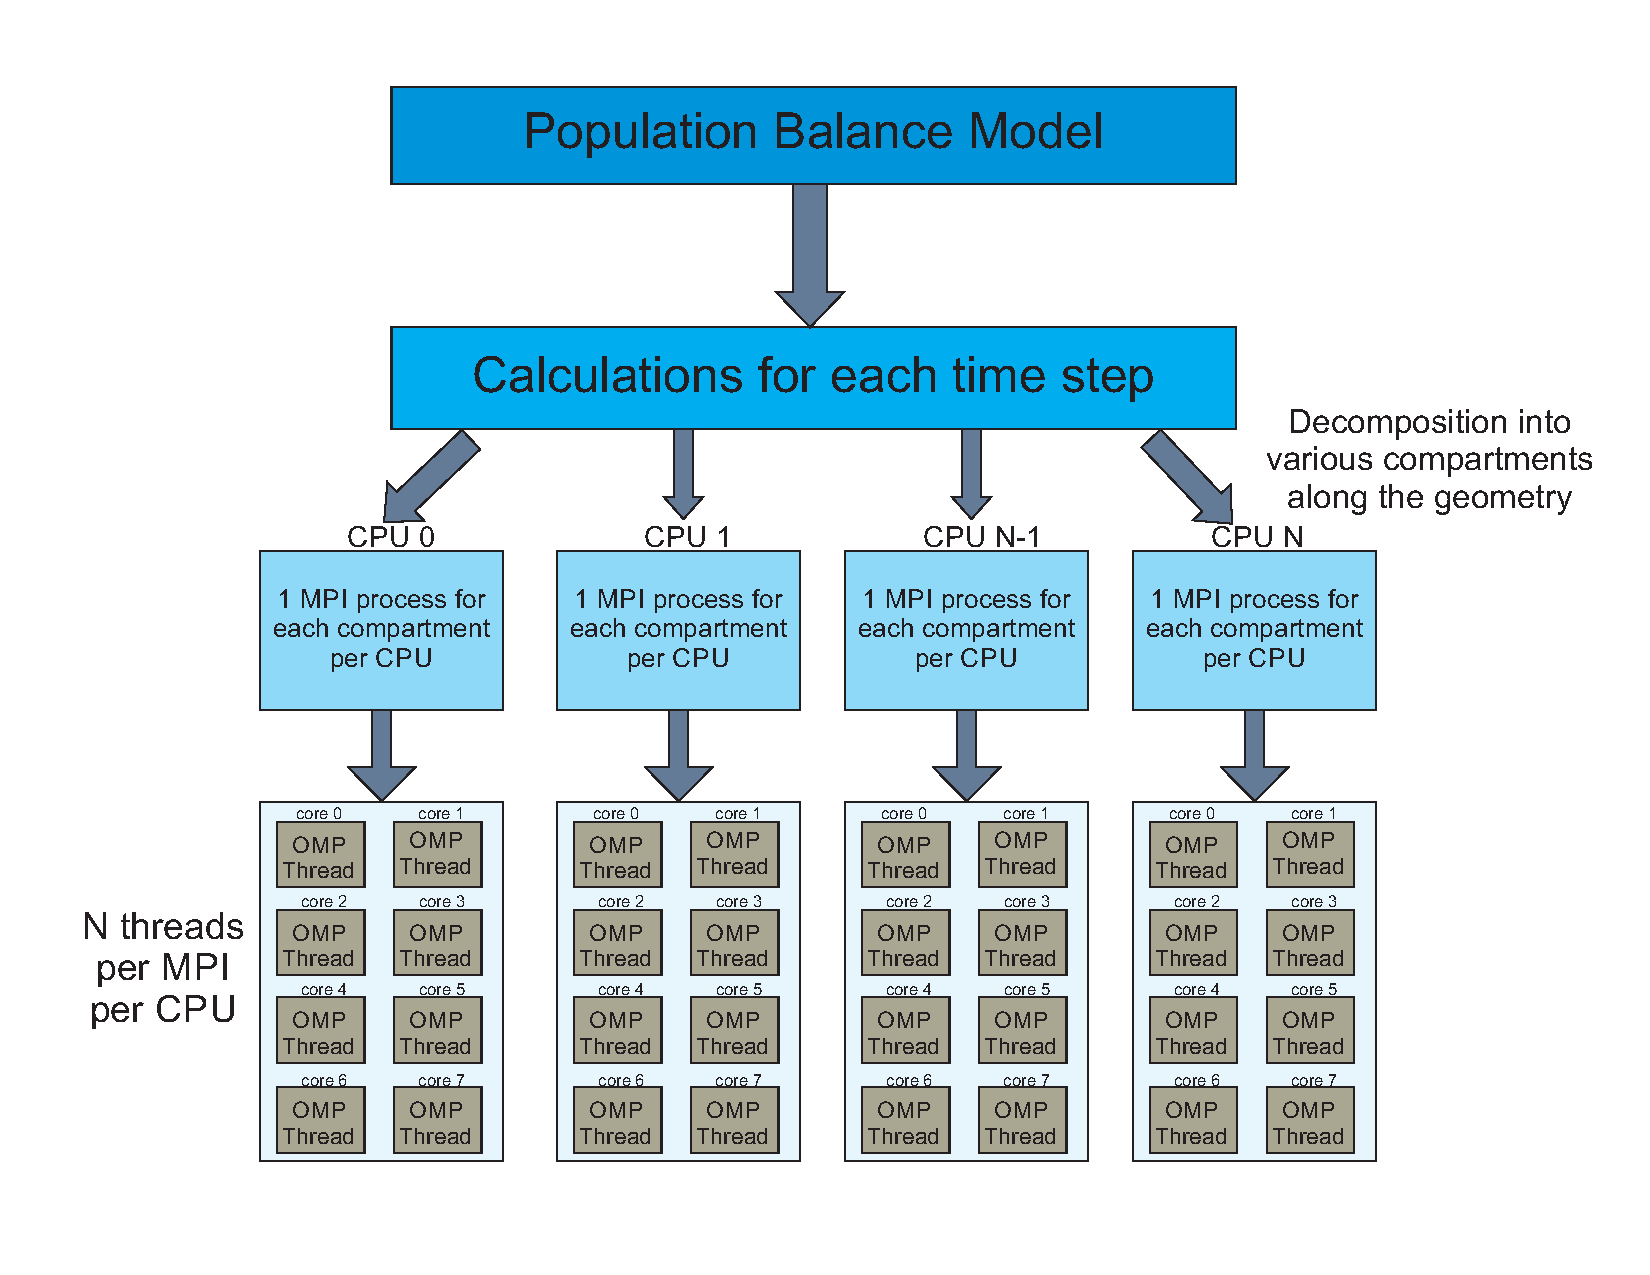
\includegraphics[scale=0.45]{PBM_decomposition.pdf}
\caption{The distribution of the PBM calculations to utilize the MPI + OMP parallelization technique on the CPUs of each node}
\label{fig:mthds_PBM_decompostion}
\end{figure}

\begin{algorithm}
     \scriptsize
     \caption{Parallel Population Balance Model}
     \label{alg:parallelPBM}
     \begin{algorithmic}[1]
     \Procedure{Population Balance Model}{$N_{Comp}$,$N_{MPI}$,$N_{OMP}$}\Comment{$N_{Comp}$ is the number of compartments}
     \State \texttt{Divide $N_{Comp}$ in $N_{MPI}$}
     \While{$t < t_{final}$}
     \For{$\forall n_{Comp}$ in 1 MPI process}
     \For{$\forall n$ in $N_{OMP}$}
     \State \texttt{Calculate $\Re_{agg}$ for solid bins $s_1$,$s_2$}
     \EndFor 
     \State \texttt{Calculate $n_{particles}$ using Euler's method}
     \EndFor
     \State \texttt{Collect $n_{particles}$ from $N_{MPI}$}\Comment{Master process collects all data}
     \State \texttt{Calculate $timestep$ using \textit{CFL} condition}
     \State \texttt{$t_{new} = t + timestep$ }
     \EndWhile
     \EndProcedure
     \end{algorithmic}
 \label{alg:parpbm}
 \end{algorithm}     


\gpnote{I do not think you have to
give a reason this specific for the selected resource. Stampede2 supports the requirements of the
software, and as a result it is the selected resource for the experiments}
The execution of the PBM was done on the
newer Stampede2 supercomputer as it supported the developed PBM C++ code. 
Each of the compute node of the cluster
consists of Intel Xeon Phi 7250 (\textquotedblleft Knights
Landing\textquotedblright) which has 68 cores on a single socket clocked at
1.4 GHz, with 96 GB of DDR4 RAM. Each of the cores consists of 4 hardware
threads. The simulations were then run by varying the the number of MPI
processes from 1 to 16 and the number of OMP threads from 1 to 8, thus, using
a maximum of 128 cores.

\subsection{CyberInfrastructre: RADICAL-Pilot (RP) \& Coupled DEM and PBM communication}
\label{sec:RPandCommunications}

\jhanote{Giannis: I believe a diagram here would be helfpul. It can go next to Figure 4. That would help distinguish the different levels/types of parallelism.}\jhanote{references missing}
RADICAL-Pilot defines a number of abstractions to describe resources, and
computational tasks. The Pilot Description is the abstraction that describes
resources by defining the number of cores, the HPC resource, and the total time that 
the resources are needed. Computational tasks are defined via the Compute Unit 
(CU) abstraction. A CU defines the executable, the necessary
environment that is needed during execution, execution arguments, and any file
dependencies the executable may have. RP also defines two managing components,
the Pilot Manager, and Unit Manager. The Pilot Manager is responsible for
submitting and monitoring a Pilot. The Unit Manager is responsible for
placing CUs in active Pilots. As soon as a Unit is placed in a Pilot, it starts
executing.

RADICAL-Pilot is utilized to execute and monitor DEM and PBM simulations.
Initially, a pilot description is created to use several cores of a resource
and submitted to the pilot manager. A CU description is created for the DEM
simulation and submitted to the Unit Manager. As soon as the pilot is active,
the DEM simulation starts executing. When it is finished the DEM output is linked to 
the new CU describing the PBM
simulation. The PBM is submitted by the Unit Manager and starts executing. Any data
dependency is satisfied by doing the necessary file linking through the CU
description.

%\gpnote{This paragraph is very similar to the previous one. Can they become
%    one?}
%The DEM and PBM executables are pre-placed in the resource along with any
%initial information required by the DEM simulation. The DEM unit creates links
%for the data files that are be needed and calls the
%executable. When the execution finishes, new links with the output are created
%in a shared space. The PBM unit uses those links to read the necessary data to
%execute the simulation. When both have finished RP downloads the PBM results.



\section{Results \& Discussion}
\label{sec:Results}
\subsection{Discrete Element Modeling (DEM)}
\subsubsection{DEM Spatial Decomposition Studies}
LIGGGHTS as discussed previously, statically decomposes the work space and
each section is sent to a MPI process for calculations. Thus, the division of
the space became an important criteria for the simulation for efficient load
balancing. The initial timing studies for the decomposition were performed using 64
cores. The time values indicated that dividing the
x-direction in more number of compartments decreased the speed of the simulation. 
% \jhanote{increasing the "speed of the simulation" is typically
% associated with improved performance. what you mean here is the converse,
% greater the number of compartments, slower the simulation? please clarify or
% fix.} \csnote{A good spot! I meant the converse. Have fixed the 2 following lines as well} 
The extra slicing in the x-direction decreased the amount of computation carried out by 
a single process but it increased the number of communications in between the MPI slave 
and master processes. This led to slower simulations when the number of slices 
increased beyond 16 in the x-direction. 
%This is easy to comprehend since the granulator has its length parallel to the x-axis. 
The studies also indicated that if the geometry is divided into more than 2 compartments 
in either the y-axis or the z-axis the simulation time increased. 
\jhanote{this is still not easy to see from table 3} \csnote{the old table does not exist anymore thus no reference}
This can be accounted to increased communication required to transfer 
the rotating impeller mesh from one compartment in the y-axis or the z-axis 
to the another compartment for each time step. Since MPI has to pass explicit 
messages in between the nodes for it to communicate data, there was a delay 
associated with the master process to obtain all the data. The master process
needed to wait for all the other processes to complete their task before it received 
the data from all other processes. With the increased 
partitions in the y and the z-axes, the master process needed to wait for more 
processes, leading to delays before the next time step could be simulated which 
in turn made the simulation slower.
%\jhanote{this sentence does 
%not make sense. MPI is "not limited": it is the message passing interface. 
%please rewrite and make consistent with data in table 3, or clarify} \gpnote{This means
%that you used blocking communication. If there is a reason for using those and not non-blocking
%communication, please include it. It gives the sense that MPI communication is blocking 
%no matter what, which is not true}
%\csnote{have explained the communications in a better manner} 
Following the results from the initial timing studies,the y and the z-axes were not divided
in more than 2 compartments for 128 and 256 core simulation as well. This
meant that the x-axis was divided into 32 and 64 compartments respectively. 

%\begin{table}
%\caption{The effect of spatial decomposition on the performance of the DEM simulations using 64 cores.}
%\label{table:rslts_dem_slicing_studies}
%\begin{center}
%\begin{tabulary}{\linewidth}{C|C|C|C}
%  
%\hline
%\bf{Slices in x-direction}&\bf{Slices in y-direction}&\bf{Slices in z-direction}& \bf{Time taken for a 0.5 
%second simulation (in minutes)}\\
%\hline
%$64$ & $1$ & $1$ & $10.27$\\
%$32$ & $2$ & $1$ & $8.70$\\
%$16$ & $2$ & $2$ & $6.83$\\
%$8$ & $4$ & $2$ & $7.20$\\		  
%$8$ & $2$ & $4$ & $7.96$\\
%\hline  		  
%\end{tabulary}
%\end{center}
%      
%\end{table}

%When MPI is used for parallelization of a task, load balancing becomes an
%important parameter that needs to be considered. When the geometry is divided,
%the amount of computation done by one core should be similar to other
%processors. 
\jhanote{What evidence/indication is there that load balancing is
a problem, as opposed to communication limited?} 
\csnote{The first few lines 
are  just general statements I could do away with this paragraph altogether. 
It does not fit with the flow} %This helps better utilization
%of the resources as well as make the simulations run faster. 
%Following the results from the initial timing studies,the y and the z-axes were not divided
%in more than 2 compartments for 128 and 256 core simulation as well. This
%meant that the x-axis was divided into 32 and 64 compartments respectively. 
\jhanote{1 paragraph, 1 idea. Is the following part of the above 'load balancing' or is 
now about 'communication'?} \csnote{tried to clear the air by removing the general statements} 
In order to avoid the expensive communication
between the processes, LIGGGHTS tries to insert the particles towards the
center of the compartment such that the number of ghost atoms are minimized.
For simulations with higher number of cores the extra slicing in the x direction 
reduced the space available for the insertion of the particles.
%This made LIGGGHTS carry out larger number of Monte-Carlo simulations to insert 
%the particles in the desired area. In some cases, the Monte-Carlo iterations performed 
%were not enough leading to many of the particles being inserted incorrectly.
This resulted in more Monte-Carlo insertion re-attempts of the particles at the desired space 
thereby increasing simulation time.
\jhanote{please elaborate} 
%Another abnormal behavior observed due to this over slicing 
%was that the particles halted in a certain compartment and
%no particle traveled beyond this compartment in the x-direction. 
Thus, the number of partitions in the x-direction were reduced and a new set of 
experiments with different 3-D partition configuration were carried out. 
\jhanote{I'm
confused: the previous sentences imply a functional problem. The next sentence
suggests a performance solution. Doesn't make sense to me.} 
\csnote{edited structure of the paragraph}
The comparison of the simulation times of experiments with the new configurations are shown in
Table~\ref{table:rslts_dem_128_256_decomp}.

\begin{table}
\caption{Comparison of time taken for the DEM simulations using 128 and 256 core due to different spatial decomposition 
configurations.}
\label{table:rslts_dem_128_256_decomp}
\begin{center}
\begin{tabulary}{\linewidth}{C|C|C|C|C}
  
\hline
\bf{Number of cores used}&\bf{Slices in x-direction}&\bf{Slices in y-direction}&\bf{Slices in 
z-direction}& \bf{Time taken for a 10 second simulation (in minutes)}\\
\hline
$128$ & $16$ & $2$ & $4$ & $264.67$\\
$128$ & $16$ & $4$ & $2$ & $247.2$\\
$256$ & $16$ & $2$ & $8$ & $271.5$\\		  
$256$ & $16$ & $8$ & $2$ & $252$\\
$256$ & $16$ & $4$ & $4$ & $265.32$\\
\hline  		  
\end{tabulary}
\end{center}
      
\end{table}
The simulation times illustrated in Table~\ref{table:rslts_dem_128_256_decomp}
show that incorrect slicing of the geometry also affected the performance of the
system. It can be noted that slicing along y-axis is more favorable than
slicing along the z-direction. \jhanote{Without further
discussion/explanation, it is difficult to discern how/why?.} \csnote{Proceeding lines 
have this discussion}\gpnote{I think there are too many "thus"s and "so"s. I think it
would read better if this was before the previous sentences and remove all "thus"s} \csnote {edited} \\
The insertion of particles is hindered when the geometry is cut along the z-axis
as the inlet is perpendicular to it. This made LIGGGHTS provision less space for
the insertion of these particles, which increased the time of the simulation.
Thus, slicing the geometry into 2 sections along the z-axis is preferred.
The chosen configurations for the final simulations consisted of the
geometry having only 2 sections in the z-direction and more slices along the y-axis.

\subsubsection{DEM Performance}
DEM simulation times were compared using a mono-sized particles of 2mm. The times plotted in
Figure~\ref{fig:rslts_DEM_2mm_timing} indicated that using lower number of
cores is not feasible for long simulations. The time taken while using 1
core is about $11$x times slower than a 128 core simulations. 
Thus, the simulations were carried out in core configurations of 64, 
128 and 256 cores. The studies undertaken had 5 mono-sized population 
of particles of diameter 0.63, 1, 1.26, 1.59 and 2 mm simulations 
and one simulation consisted of particle size distribution. 
Figure~\ref{fig:rslts_DEM_timing_studies} shows that the amount of wall clock time
required for a 10 second simulation of the granulator. The post processing
MATLAB script was run on the dump files obtained from the simulation and it
was observed that the system reached a steady state about 4-6 seconds of the
simulation time. Particles with larger diameter reached steady state at a
faster rate with an average hold-up of particles of about 6500.

\begin{figure}
\begin{subfigure}{.45\textwidth}
\centering
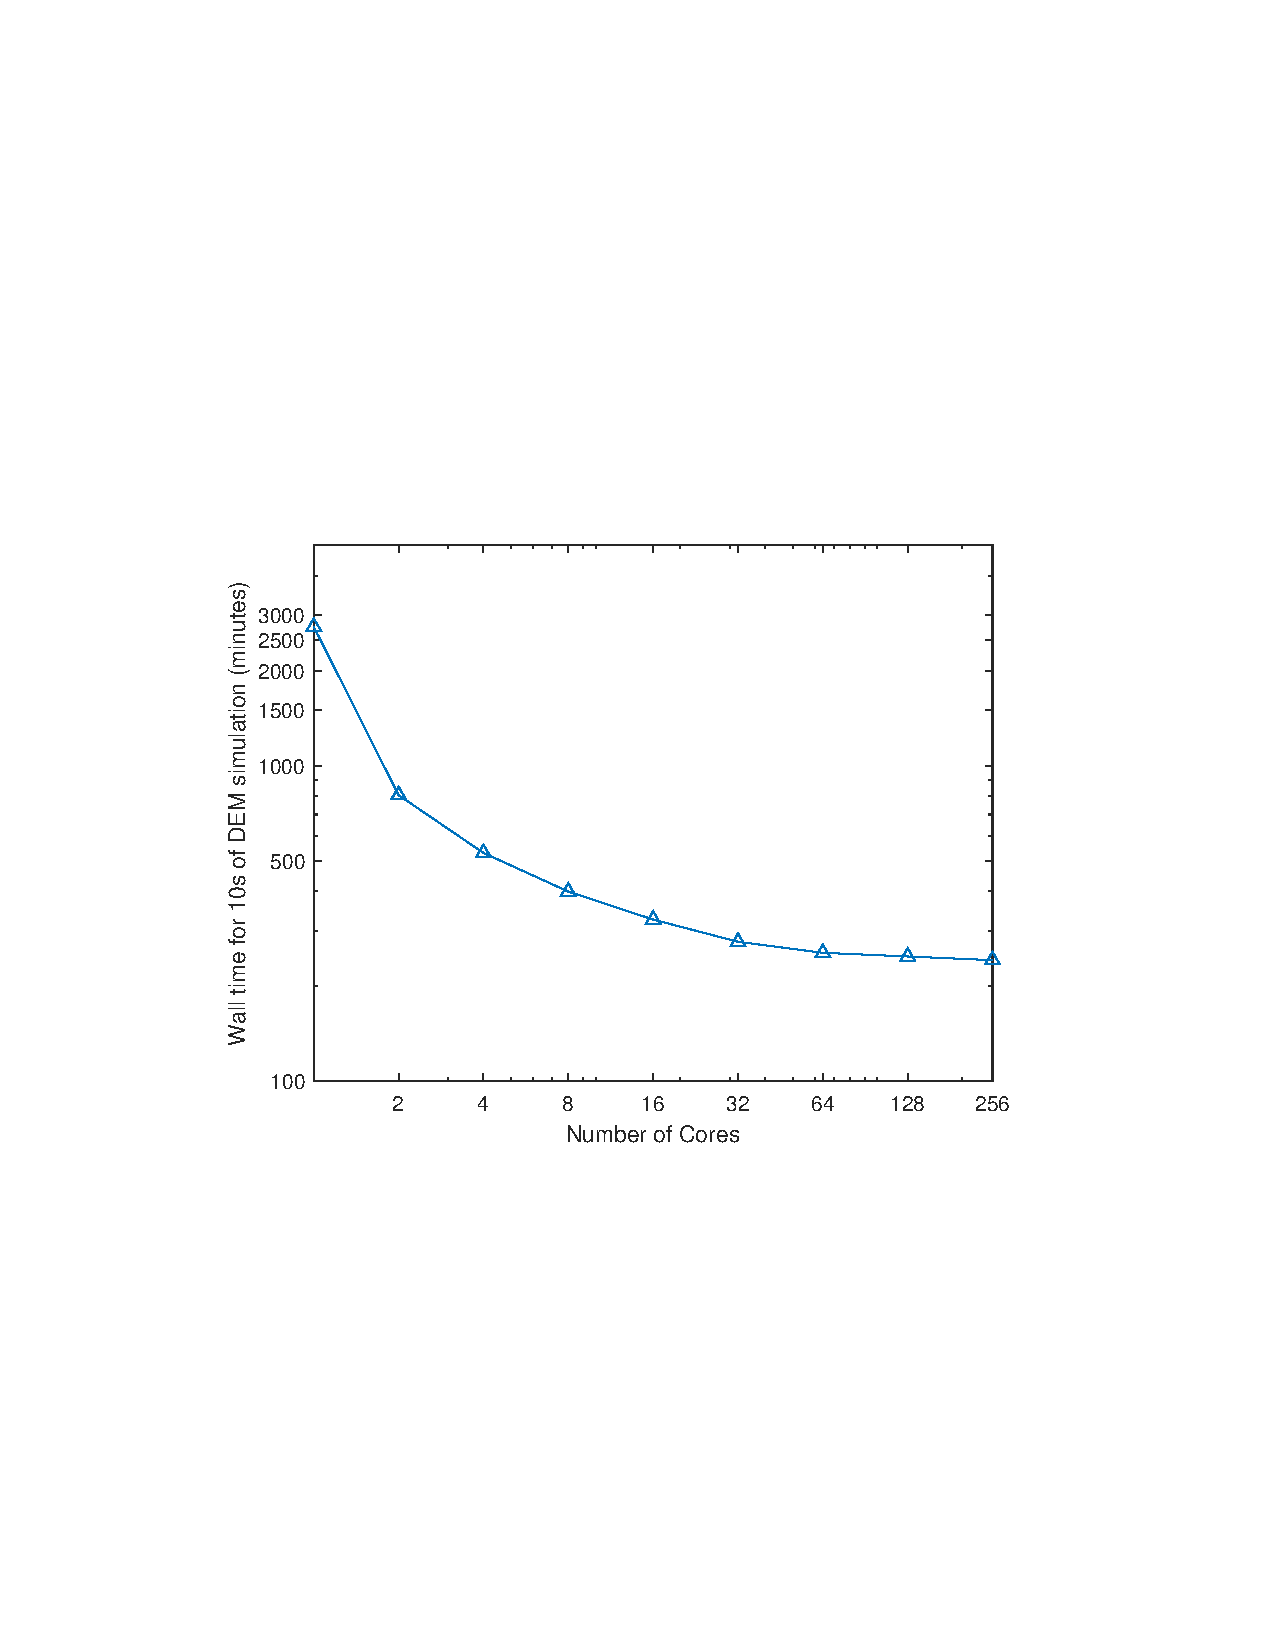
\includegraphics[scale=0.6]{rslsts_2mm_timing_mtlb.pdf}
\caption{}
\label{fig:rslts_DEM_2mm_timing}
\end{subfigure}\hfill
\begin{subfigure}{.45\textwidth}
\centering
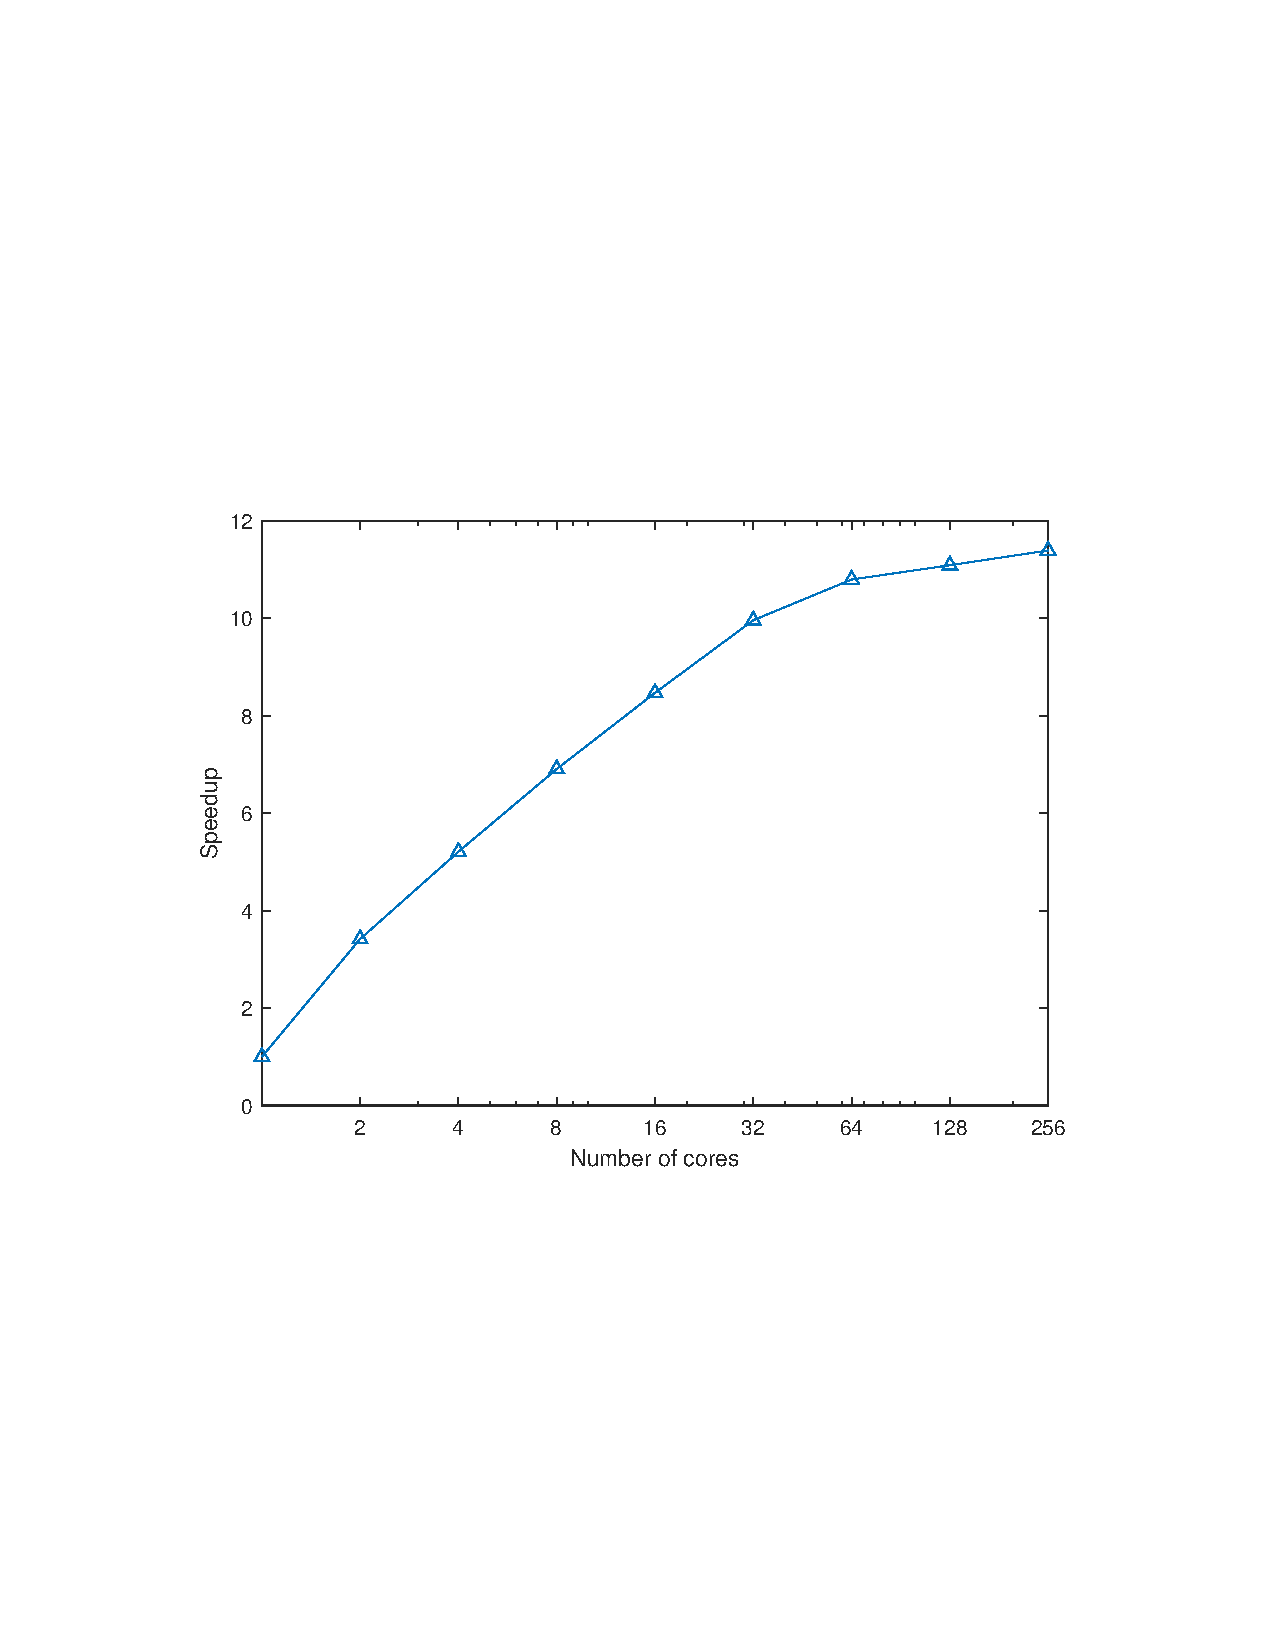
\includegraphics[scale=0.6]{rslsts_2mm_DEM_speedup_mtlb.pdf}
\caption{}
\label{fig:rslts_DEM_speedup}
\end{subfigure}
\caption{(a) The variation in the amount of time taken for the DEM simulation of 2 mm particles as 
a function of number of cores. The improvements in the speed of the simulation was higher when the 
cores were increased from 1 to 16 when compared to speed improvements obtained with a core count greater 
than 16.(b) The speedup achieved in the DEM simulations of 2 mm particles. There 
was a linear increase up to 16 cores while the speedup seems to plateau when 
more number of cores are used due to larger amount of communications.
\jhanote{consistency in the x-axis labeling and major/minor tics please. please refrain from inconsistency across figures.}}
\end{figure} 


\gpnote{You are saying that a measure is not good to represent performance, but a function which has
this measure as a free variable is?! Showing only time may not be the best representation of performance,
but time is a good measure of performance. I do not see any data other than timing data for performance.} 

\csnote{changed}

Pure timing studies are not the best representation for the parallel performance of a program. 
Speedup of a parallel program indicates the speed increase of the program when it is run on more 
compute cores compared to the wall clock time when it is run in serial. It is the most common way to 
represent the parallel performance. Speedup is the ratio of the time taken to run the program in serial 
to the time taken by the program to run in parallel as shown in Equation~\ref{eqn:rslts_DEM_Speed_Up}. 
For an ideally parallelized program, speedup is equal to $n$, where $n$ is the number of cores used.
\gpnote{My general preference: Anything that has to do with mathematics or arithmetic, regardless if it
    is inline with the text or not, should be in \$ signs. It makes it clearer than quotes}

\begin{align}
\textit{Speedup} = \frac{\textit{Serial Wall Clock Time}}{\textit{Parallel Wall Clock Time}}\label{eqn:rslts_DEM_Speed_Up}
\end{align}

Speedup does not take into account number of processors used in the simulation. Another metric 
used to determine parallel performance is Parallel Efficiency. This metric is defined as 
speedup divided by the number of cores used. Thus, parallel efficiency normalizes speedup and gives 
the fraction of the ideal speedup a program achieves increasing the number of cores.

\begin{align}
\textit{Parallel Efficiency} = \frac{\textit{Serial Wall Clock Time}}{\textit{Parallel Wall Clock Time $\times$ $n$}}
\label{eqn:rslts_DEM_parallel_efficiency}
\end{align}

The speedup of the DEM simulations using only MPI cores is shown in Figure~\ref{fig:rslts_DEM_speedup}.
There was a linear speed increase in the speedup up to 16 cores, after which the 
performance plateaued. Figure~\ref{fig:rslts_DEM_speedup} indicates that there 
was not a significant amount of speed improvement for the simulation when 256 cores were used for the 
simulation over 128 cores. This speed decrease could be due to the communication time between 
the MPI processes. When the particles move from one section to another of the space, they are 
transferred as ghost particles from one process to another process as well as transfer the geometry 
for each time step. This led to large amounts of communications between the processes. 
One of the issues of using a cluster with no shared memory in between nodes is that it has to 
rely on the networking infrastructure of the cluster for communications leading to higher 
communication times. There are more sections present when 256 cores are used for the 
simulation, leading to more communication in this system when compared to the 128 core simulation. 
These excess communication made the simulation slower though there is more processing power and 
it required lesser time for other calculations. Another observation that made from Figure~\ref{fig:rslts_DEM_timing_studies} was that the particle size distribution simulation took more time 
compared to the simulations with mono-sized particles of 1.59mm and 2mm, though the mean size of 
particles in the distribution was 2mm. The default profile provided by LIGGGHTS indicated that the time 
spent in calculating the particle-particle interaction forces was higher than the mono-sized 
simulations. The different diameters made the interaction forces more tedious thus, making it 
computationally more expensive. 


\begin{figure}
\centering
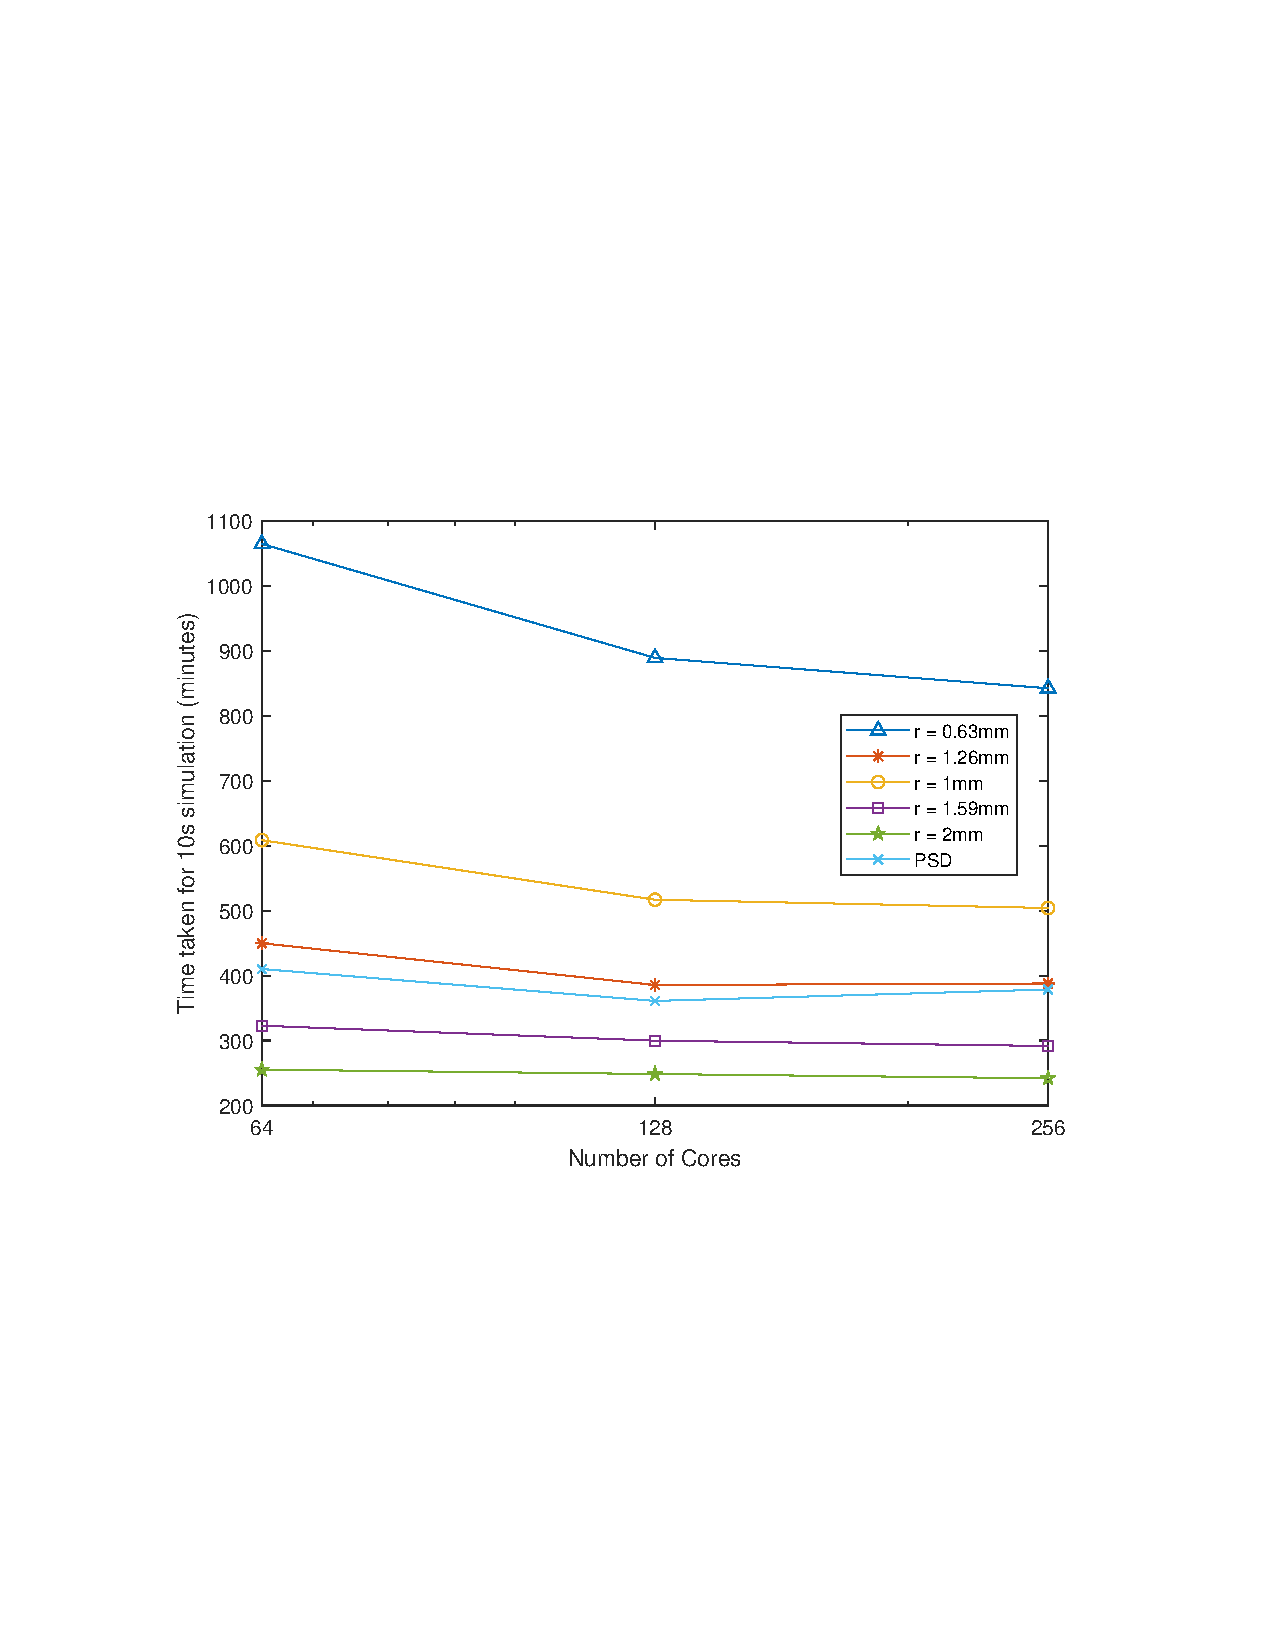
\includegraphics[scale=0.7]{rslsts_DEM_alldia_timing_mtlb.pdf}
\caption{ \jhanote{consistency in the x-axis labeling and major/minor tics please. please refrain from inconsistency across figures.}
Time taken for a 10 second DEM simulation for radii ranging from
 0.63mm to 2mm and a particle size distribution ranging from 1mm - 3mm. The speed improvements 
 for the smaller particles was higher as the core count increased when compared to the larger particles. 
 The larger number of smaller particles require more computational power thus benefit more as the number 
 of cores are increased. }
\label{fig:rslts_DEM_timing_studies}
\end{figure}

The communication time in LIGGGHTS is indicated by the Modify time, which is the sum of the 
times required to transfer the rotating mesh from one process to the other. From Figure~\ref{fig:rslts_DEM_percent_plot}, it can be seen that the main portion of the simulation time is taken up by 
the modify time. This was expected since the impeller rotates at a very high speed of 2000 rpm. If 
the number of processes are increased the amount of time spent in transferring the mesh also 
increased. In the studies, the modify time as a percentage of the simulation increased from 82\% to 
about 90\%, when the core count was increased from the 64 cores to 256 cores. But, using the 
higher number of cores reduced the time taken to calculate particle-particle interaction as well as  
neighbor calculation. Thus, 128 cores was a better implementation for meshing and decomposition of the 
geometry for faster simulations.

\begin{figure}
\centering
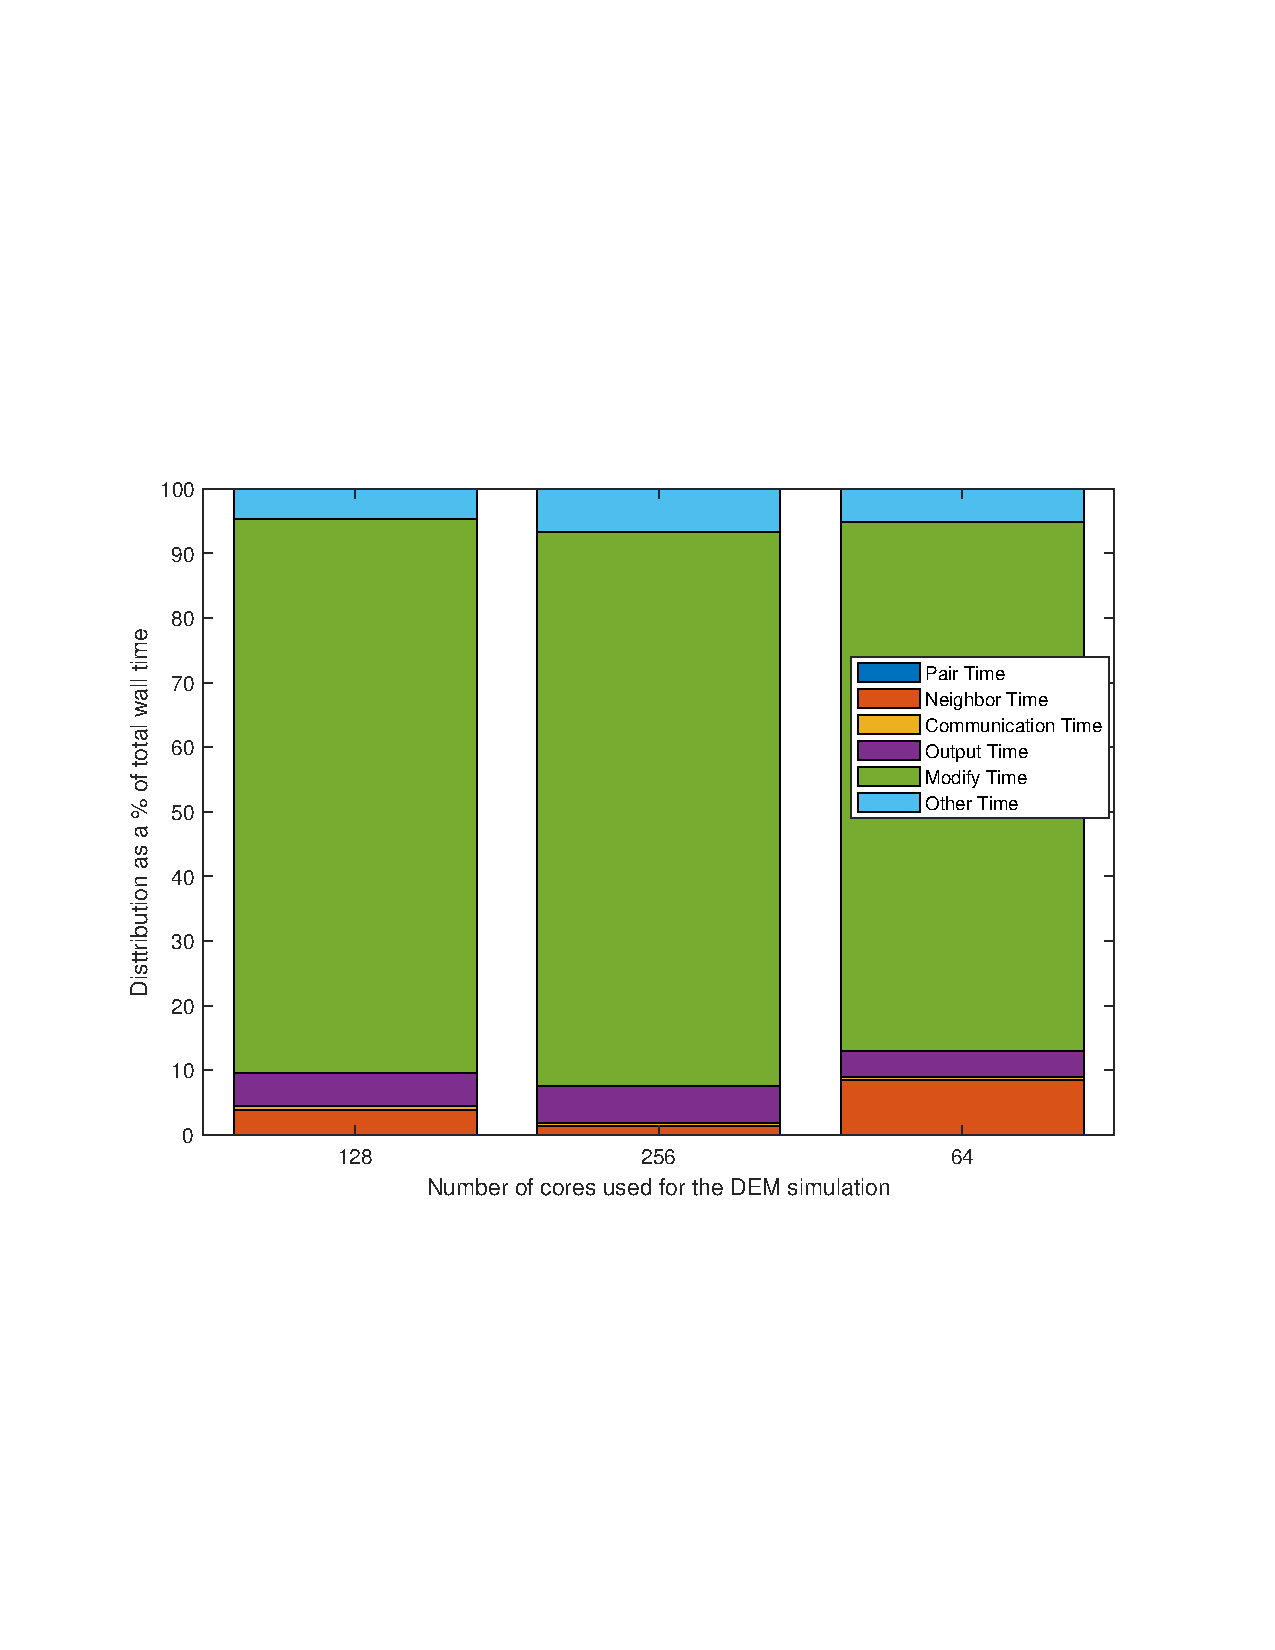
\includegraphics[scale=0.6]{rslsts_DEM_profle_mtlb.pdf}
\caption{The distribution of time taken by each component of the DEM 
simulation with varying number of cores for the 2mm particles. It 
can be observed that the percentage of time required to modify the 
geometry (indicated by the modify time), i.e. rotating the impeller 
at high speeds, was the highest.}
\label{fig:rslts_DEM_percent_plot}
\end{figure}


\subsection{Population Balance Modeling (PBM)}
\subsubsection{PBM model validation}

The population balance model implemented was considered to have an inlet flow
of particles in the first compartment at a constant mass flow rate of 15
kilograms per hour. The particles were assumed to have a log normal
distribution with minimum diameter of the particles being about 12 $\mu$m and
the maximum of 2.1 mm with a mean of 0.453 mm and a standard deviation of
about 0.62 mm.

The PBM used in this study employed an aggregation kernel that takes into
account the formation of a larger particle from only two smaller particles.
The ratio of the rate of formation and the rate of depletion due to
aggregation helped us monitor whether the PBM satisfied the conservation of
mass. Since this PBM took into account the aggregation of only 2 particles at
once, the ratio of the particles was expected to have a value of 0.5 during
the aggregation process. This ratio was reported by the PBM to be 0.5
throughout the simulation, validating the accuracy of the PBM used.

Figure~\ref{fig:rslts_PBM_d50_plots} shows four different particle size
distribution plots at four different time instants.
Figure~\ref{fig:rslts_PBM_d50_plots}(\subref{fig:30s}) shows the distribution
of the particles at 30 seconds, where we expected to have the highest number
of the smaller particles. Since the degree of aggregation that has occurred
was very low, there was a jump in the number of particles of the smaller size.
The particle size distributions at 2 intermediate times of 50 seconds and 75
seconds are plotted in Figures~\ref{fig:rslts_PBM_d50_plots}(\subref{fig:50s})
\& \ref{fig:rslts_PBM_d50_plots}(\subref{fig:75s}) respectively. These
illustrate that there was an increase in the number of larger particles  and a
subsequent decrease in the number of smaller particles.
Figure~\ref{fig:rslts_PBM_d50_plots}(\subref{fig:100s}) shows the distribution
of the particle size at the end of the granulation process. It can be seen
that the number of particles in the higher diameter bins had increased.

\jhanote{I struggle to see how this is validation. What are you validating
against? What is the measure / metric of validation?}
\csnote{The simulation is validated with the assumption that 2 particles combine 
to form 1 particle. Thus the ratio 0.5 come into the picture and this value if consistent
throughout the simulation, this validates the simulation}


\begin{figure}
\begin{subfigure}{.5\textwidth}
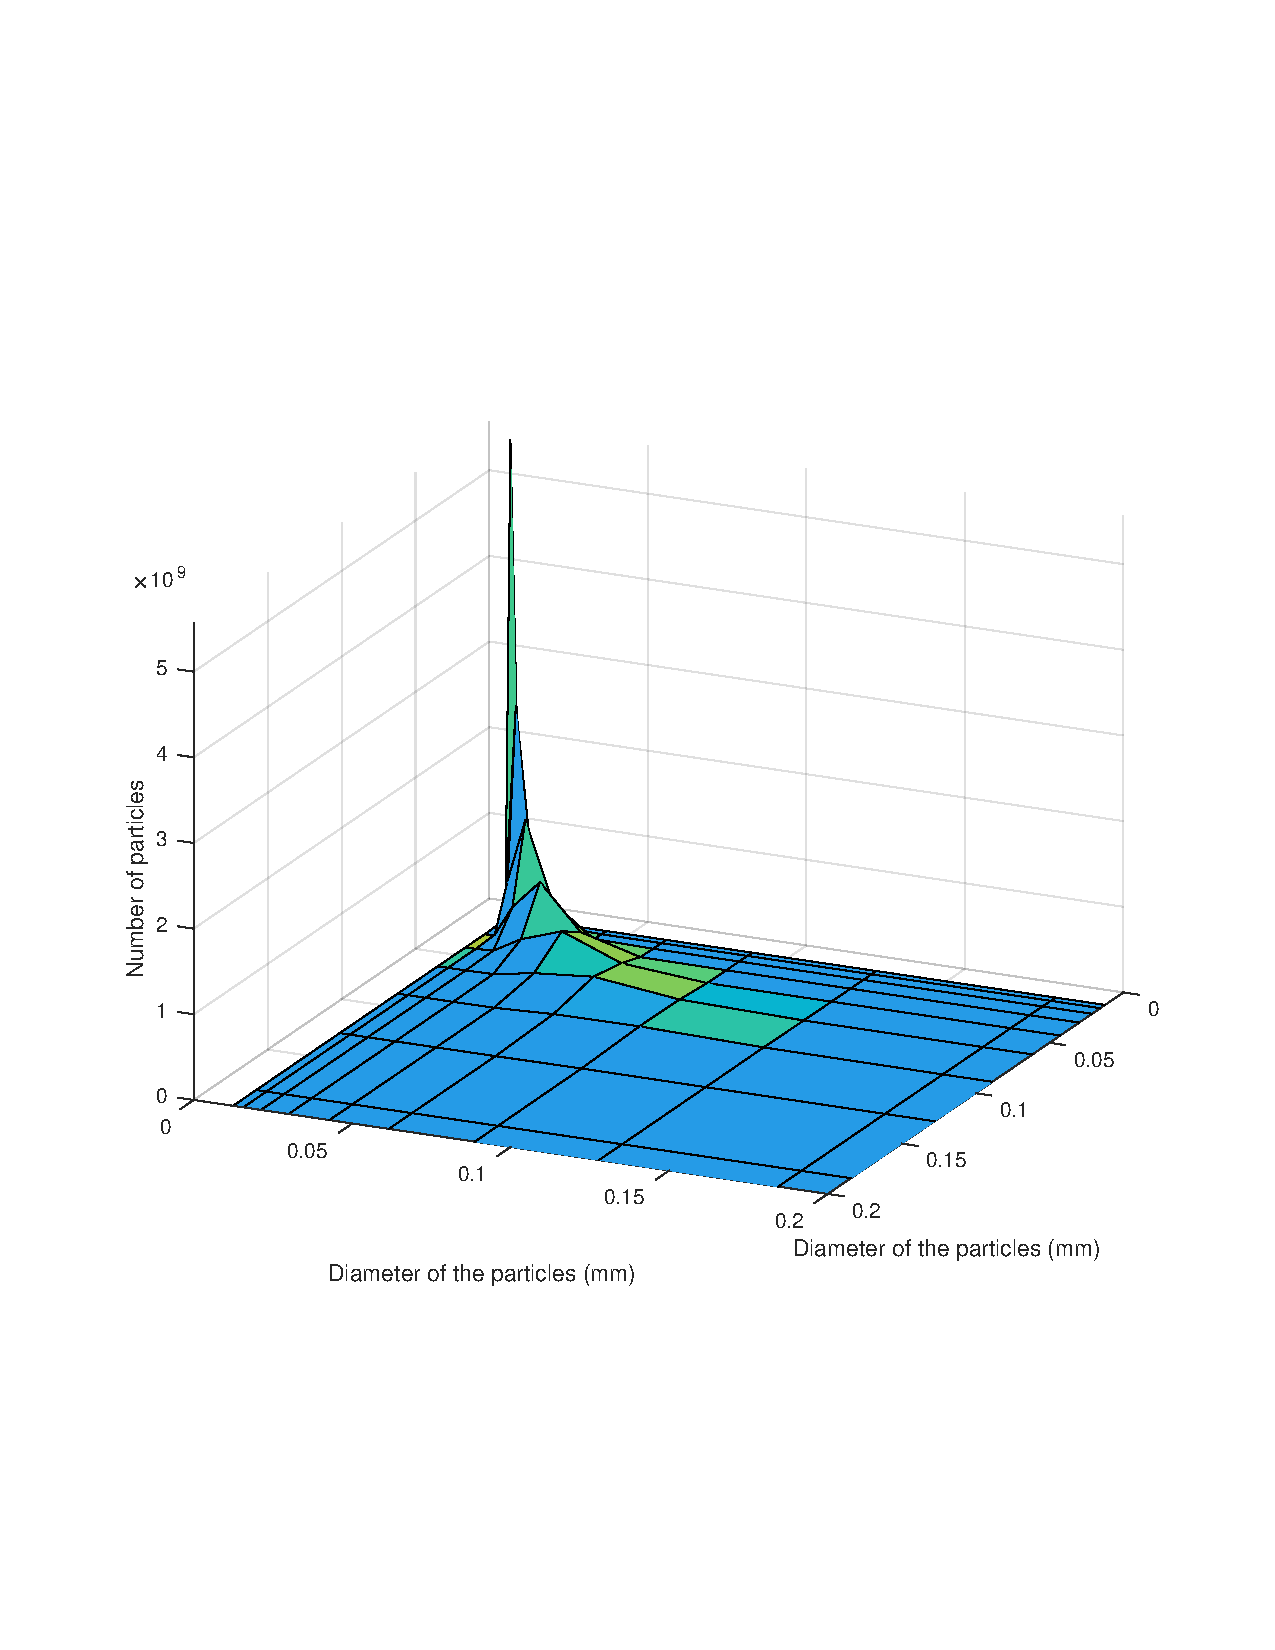
\includegraphics[scale=0.45]{rslts-PBM_30s_psd.pdf}
\caption{}	
\label{fig:30s}
\end{subfigure}\hfill
\begin{subfigure}{.5\textwidth}

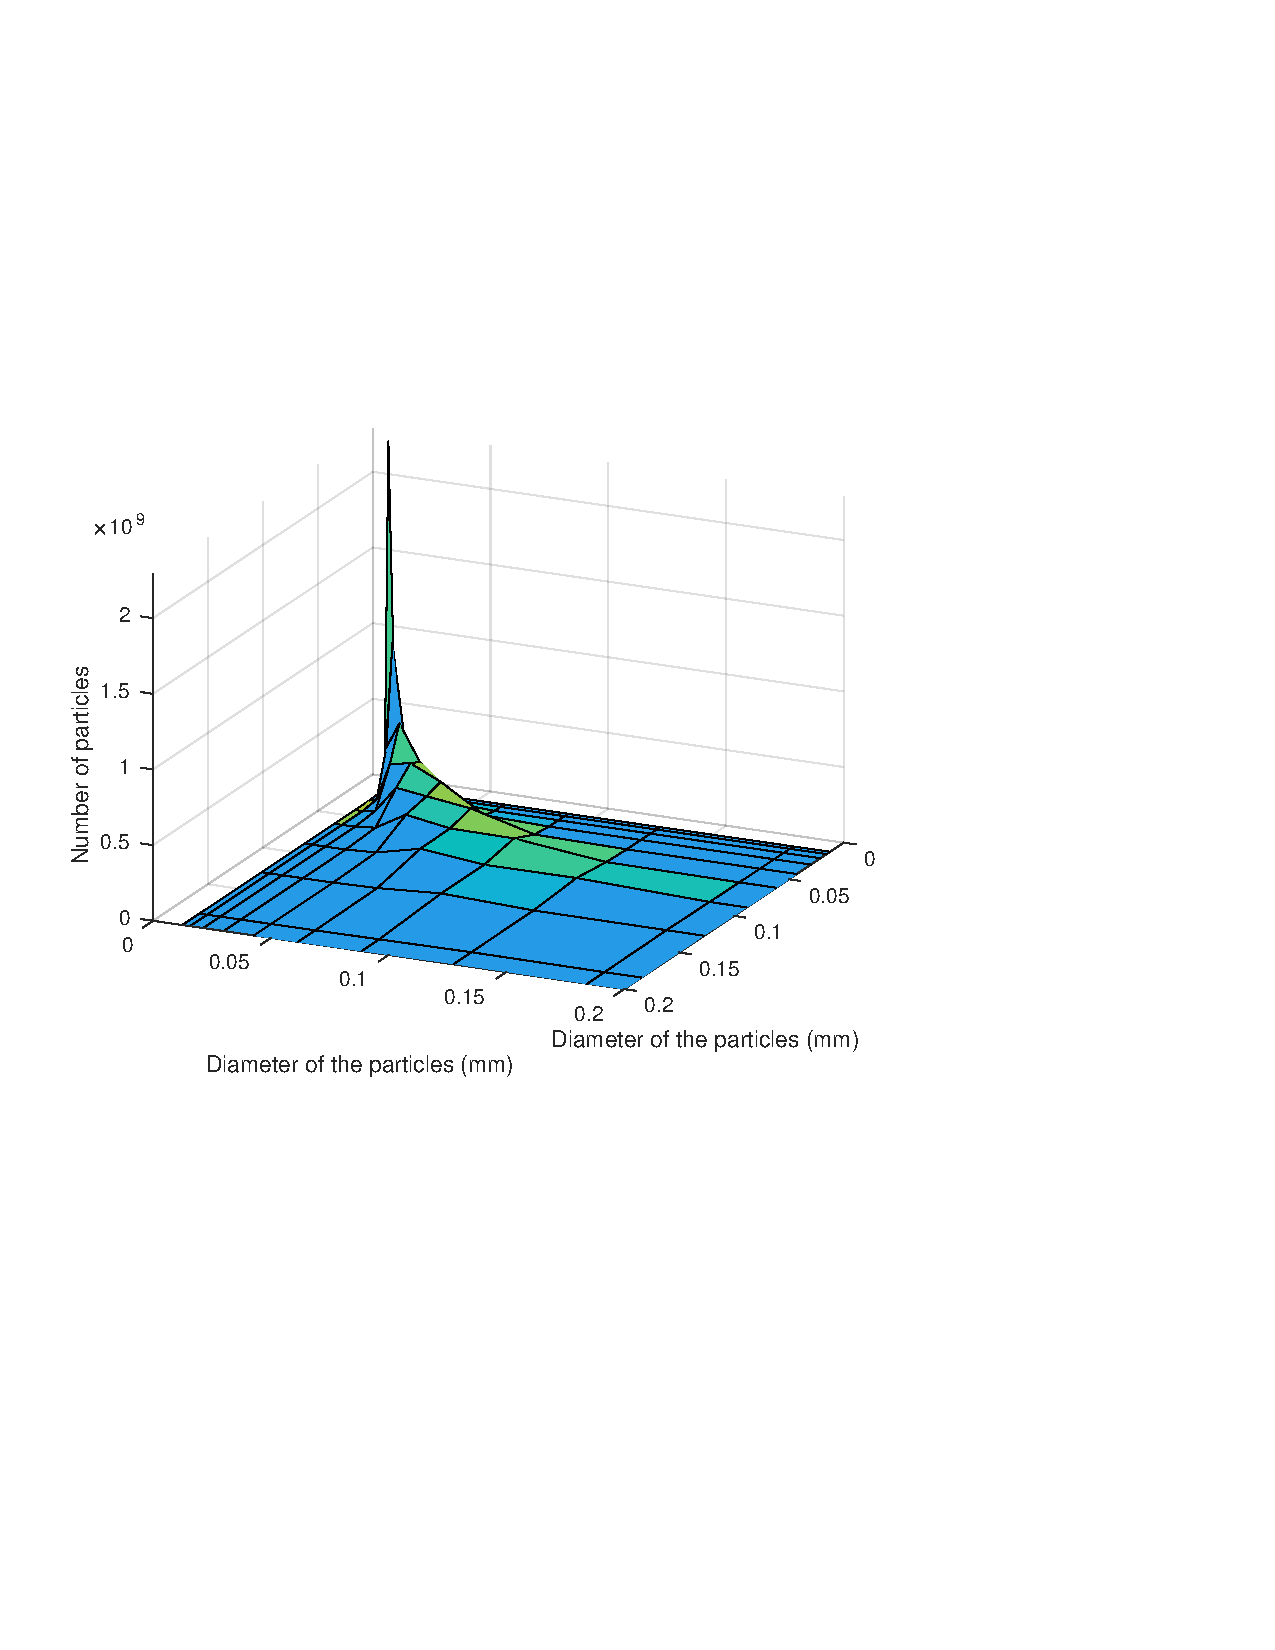
\includegraphics[scale=0.6]{rslts-PBM_50s_psd.pdf}
\caption{}
\label{fig:50s}
\end{subfigure}
\begin{subfigure}{.5\textwidth}

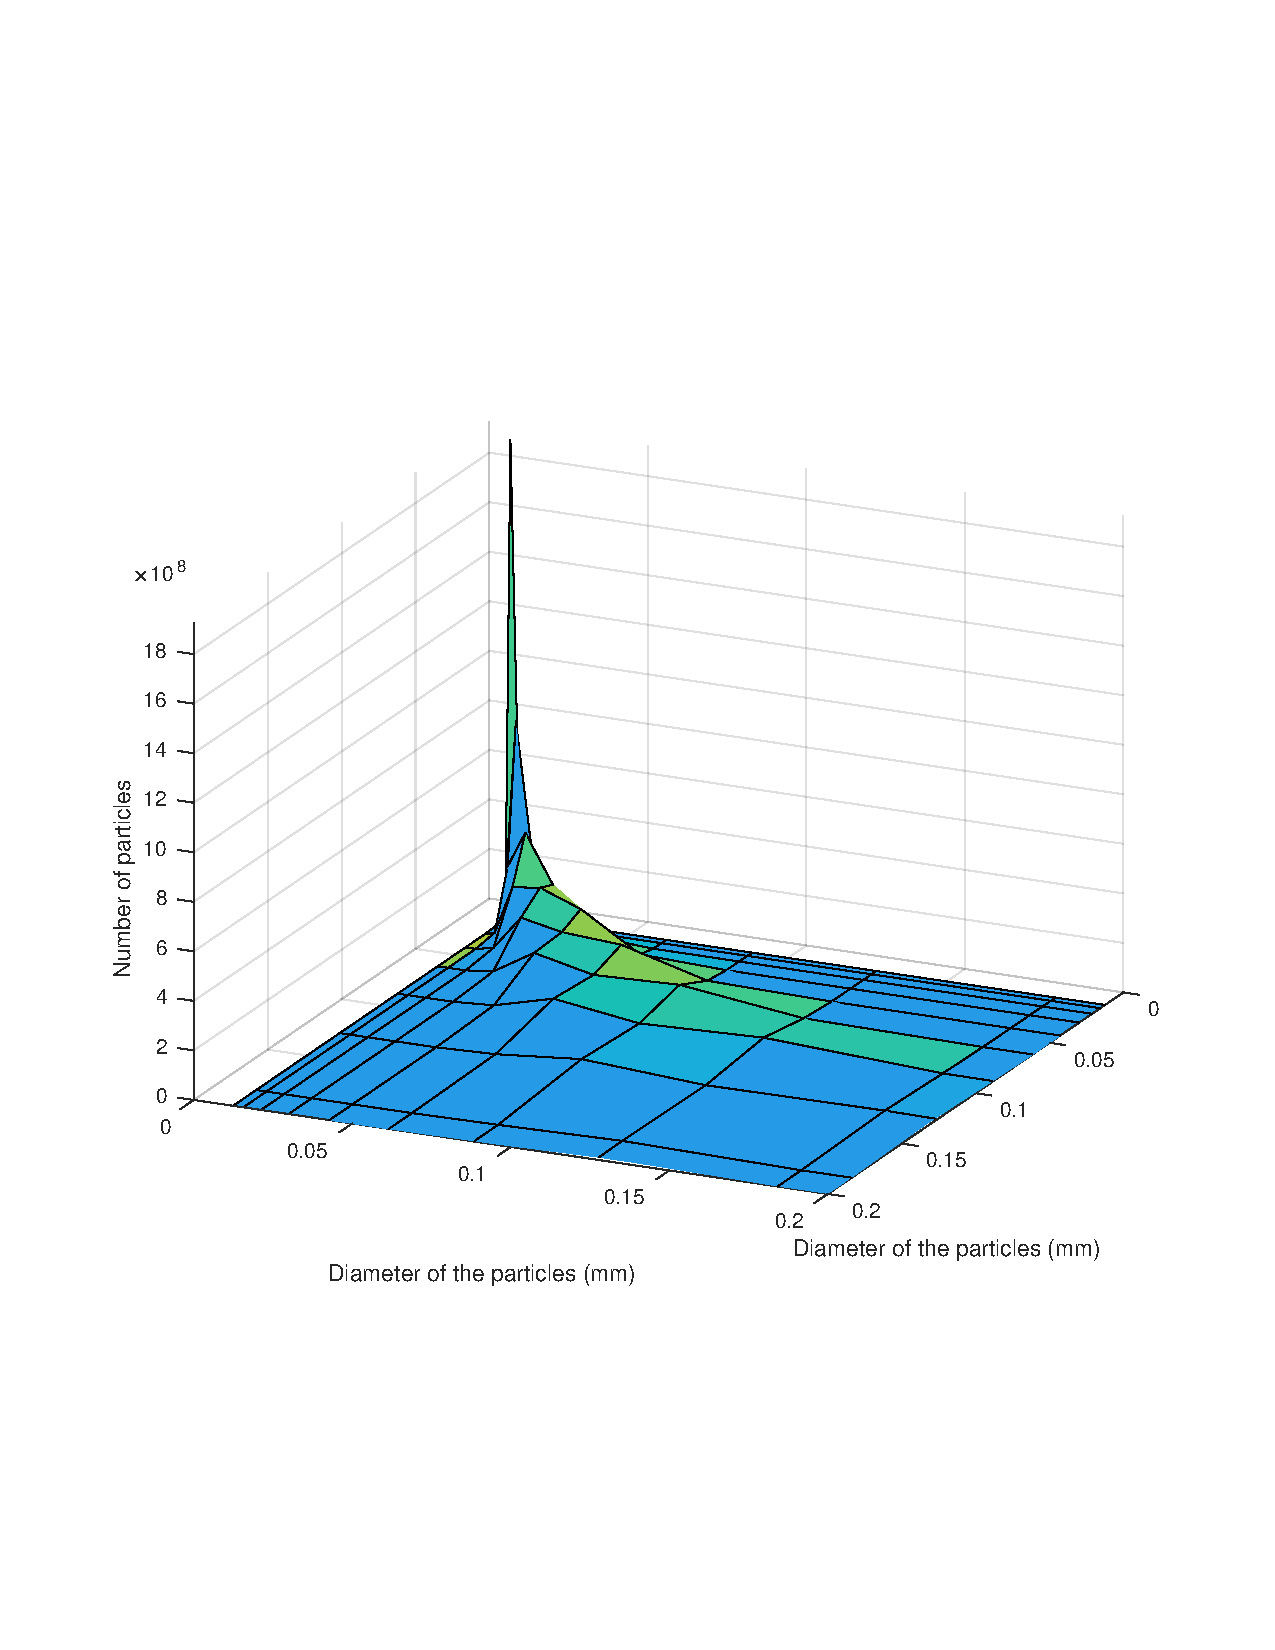
\includegraphics[scale=0.45]{rslts-PBM_75s_psd.pdf}
\caption{}
\label{fig:75s}
\end{subfigure}\hfill
\begin{subfigure}{.5\textwidth}

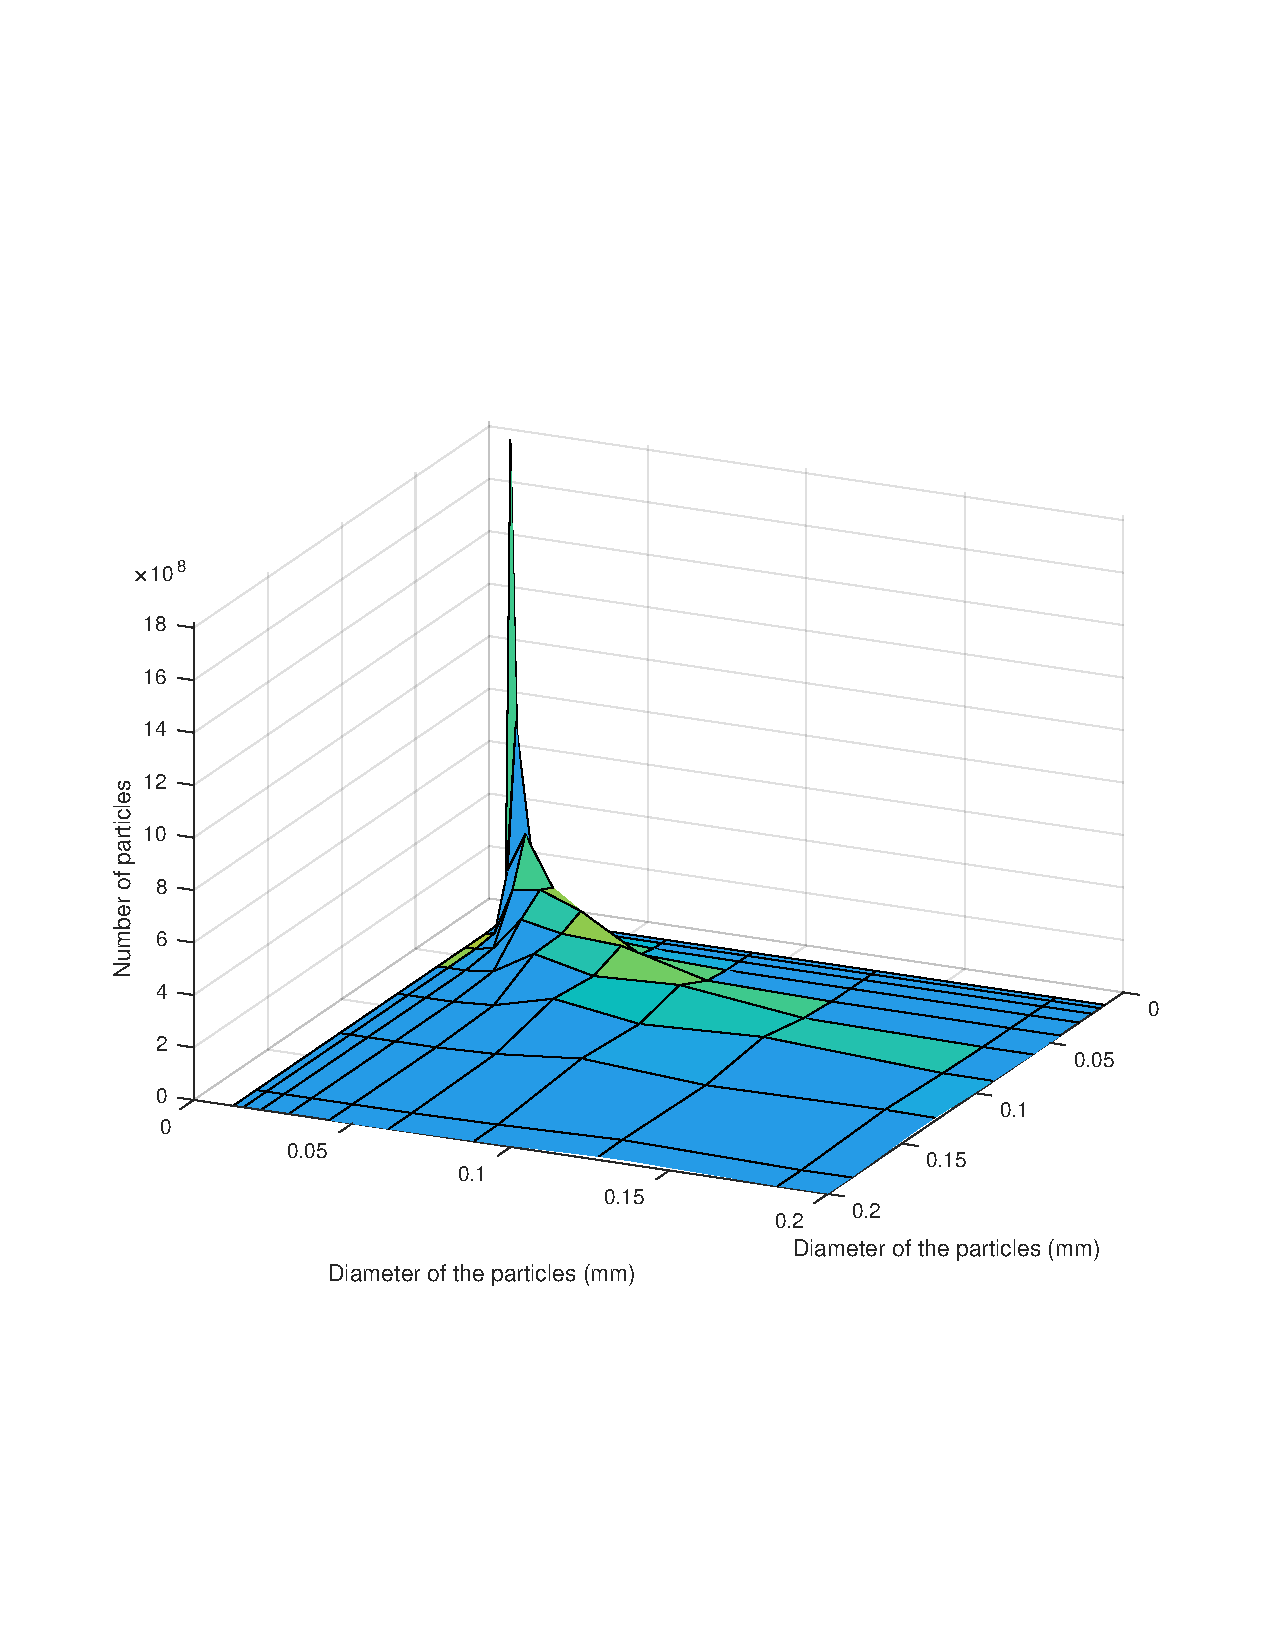
\includegraphics[scale=0.45]{rslts-PBM_100s_psd.pdf}
\caption{}
\label{fig:100s}
\end{subfigure}
\caption{Representation of the total number of particles inside all compartments with diameters less than 
0.2 mm in mm after (\subref{fig:30s}) 30s (\subref{fig:50s}) 50s (\subref{fig:75s}) 75s and
 (\subref{fig:100s}) 100s of PBM simulation (Mixing takes place for the first 25 seconds).}
\label{fig:rslts_PBM_d50_plots}
\end{figure}   

\subsubsection{Parallel PBM performance studies}
The PBM was run for the results obtained from each of the aforementioned DEM simulations. 
Since the PBM has been parallelized using hybrid techniques, a combination of MPI and OMP cores 
were used to perform the simulations. Figure~\ref{fig:rslts_PBM_timing_studies} shows the average time 
taken by a PBM simulation for a total of 100 seconds of the granulation process, which included 25 
seconds of the mixing time and 75 seconds of granulation time. The time taken for simulating all DEM 
scenarios by a single set of core configuration of in less than 10\% of each other, thus, an  average 
time for a single core configuration was used to illustrate the performance. 
These simulations were run in a varied configuration of cores ranging from 1 to 128. The cores were 
initially increased to 16 by increasing only the number of MPI processes. To increase the number of 
cores used, 8 OMP threads were employed for a configuration of 32(4 MPI  and 8 OMP), 64(8 MPI  and 8 OMP) 
and 128 cores (16 MPI  and 8 OMP). Figure~\ref{fig:rslts_PBM_timing_studies} shows that the program scaled 
well to about 32 cores but then, the improvement in the performance is negligible. The scaling with the 
only MPI cores showed substantial increase in performance.
\begin{figure}
\centering
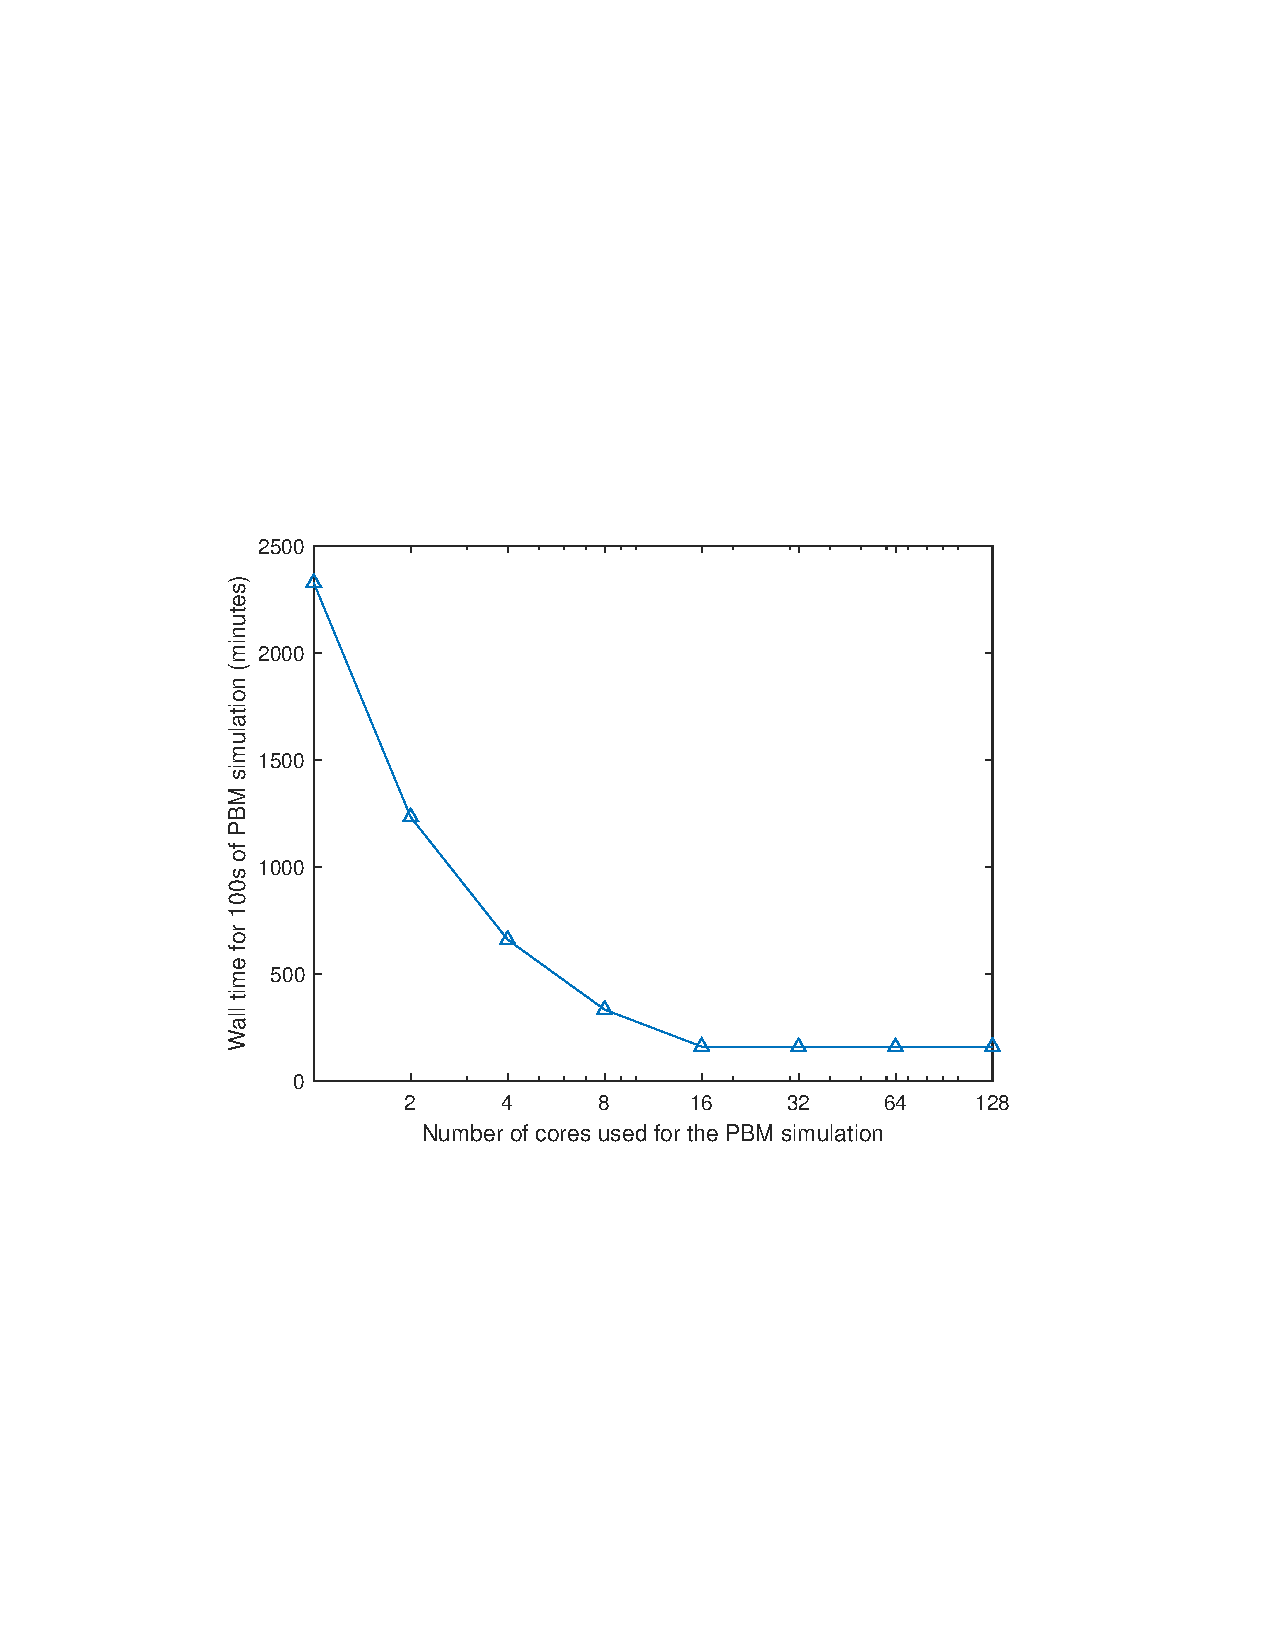
\includegraphics[scale=0.75]{rslsts_PBM_timing.pdf}
\caption{Average time taken to run the PBM simulation which consisted of 25 seconds of mixing time 
and 75 seconds of granulation time at different core configurations. There was a steady decrease as 
the number of MPI processes were increased, but the improvements on increasing the OMP threads were 
not that significant.}
\label{fig:rslts_PBM_timing_studies}
\end{figure}


Figure~\ref{fig:rslts_PBM_speed_up} depicts the speed up achieved by the hybrid parallel PBM code. It 
can be seen when the MPI cores used were increased from 1 to 16 cores the speed up achieved was 
almost linear. This speed increase was due to the way MPI has been implemented inside the code. 
Each compartment of the granulator was  offloaded on one MPI process, thus making 16 MPI processes 
the ideal since, the granulator had been divided into 16 compartments. When less than 16 cores were used, 
more than 1 compartment was sent to a single MPI process, which led to a 
decrease in performance. The implementation of OMP on top of the MPI parallelization helped improve 
the performance by the about 10\%. The calculations inside the OMP parallel section of the code 
consisted of large number of nested loop which have been known to be difficult to parallelize~\citep{He2016} 
using the native \textit{C++}'s OMP libraries. The amount of communication time spent in 
between these threads was much higher than the speed increase achieved by using higher number of 
cores. One OMP thread had to wait for another thread to complete processing the outer loops thus lower 
performance increase is achieved by using the OMP implementation. 

\begin{figure}
\begin{subfigure}{.45\textwidth}
\centering
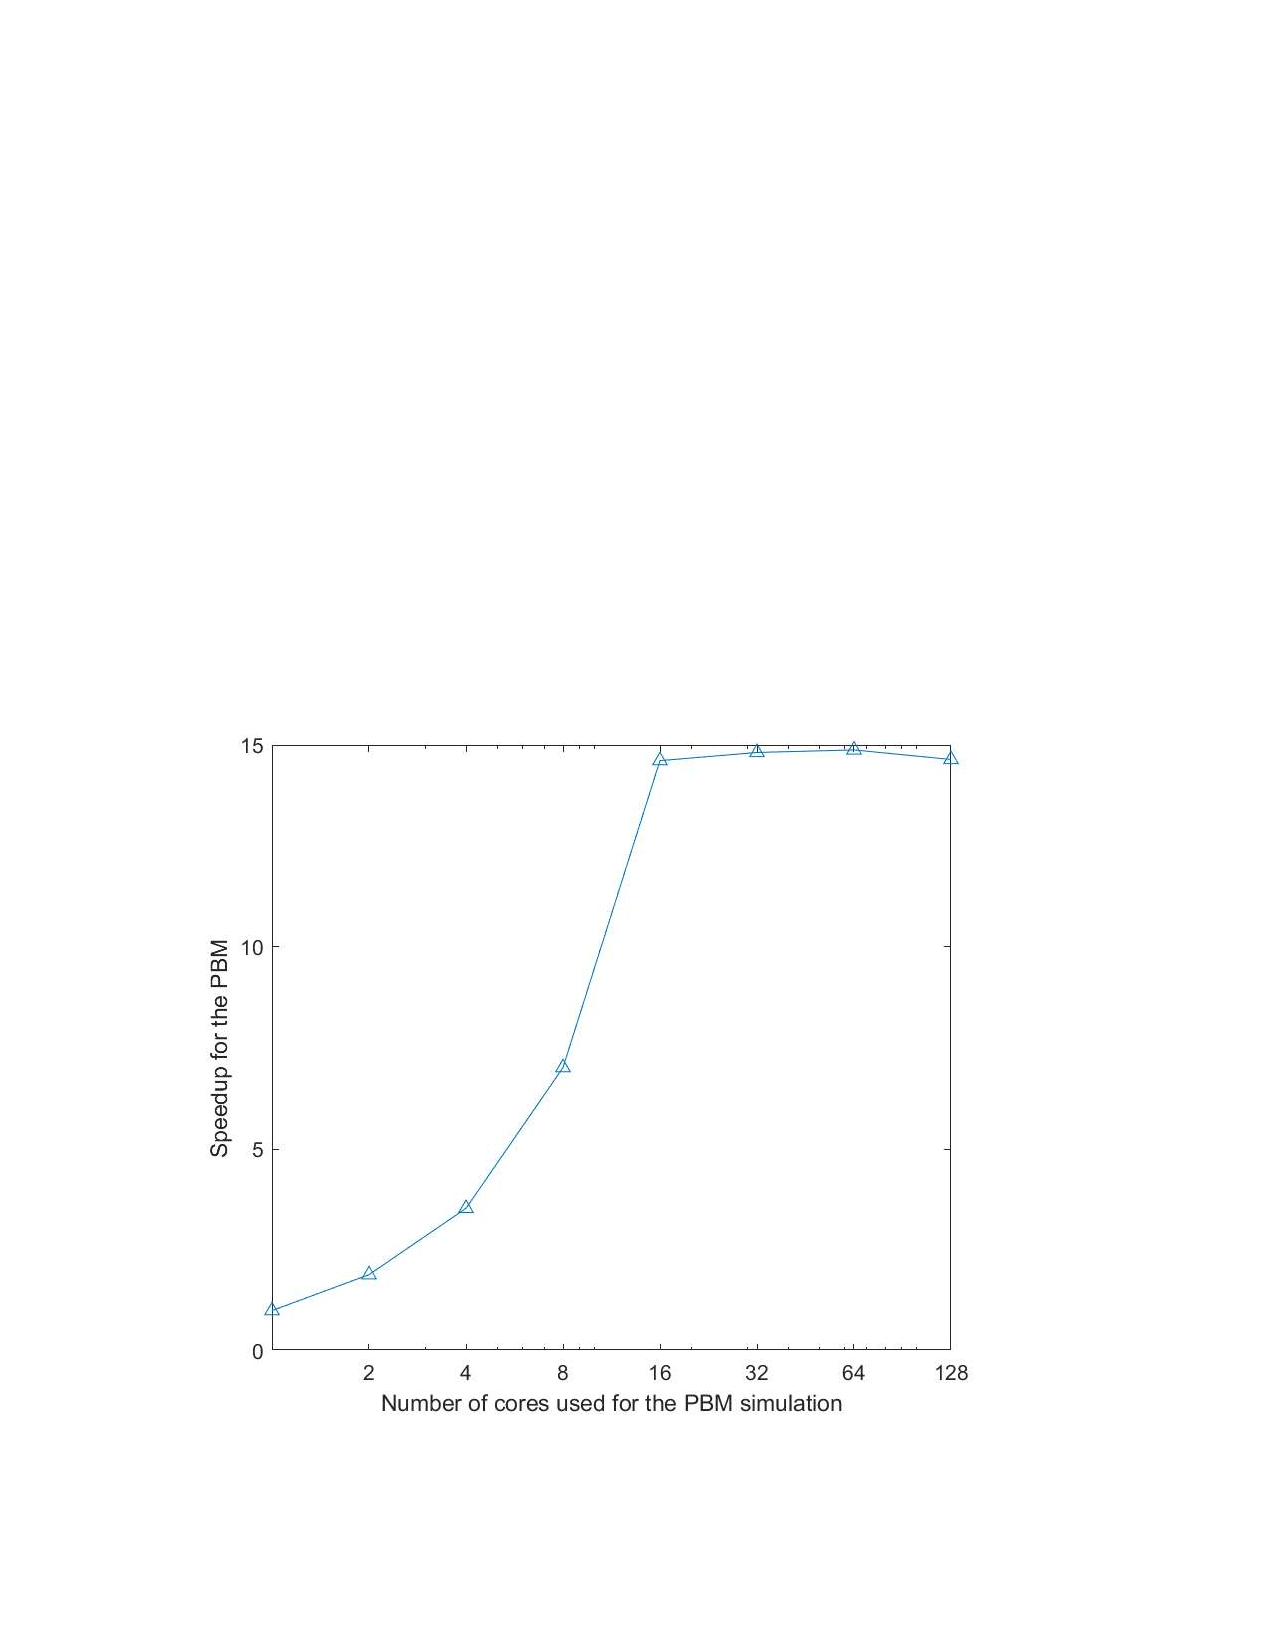
\includegraphics[scale=0.5]{rslsts_PBM_speedup_logx.pdf}
\caption{}
\label{fig:rslts_PBM_speed_up}
\end{subfigure}\hfill
\begin{subfigure}{.45\textwidth}
\centering
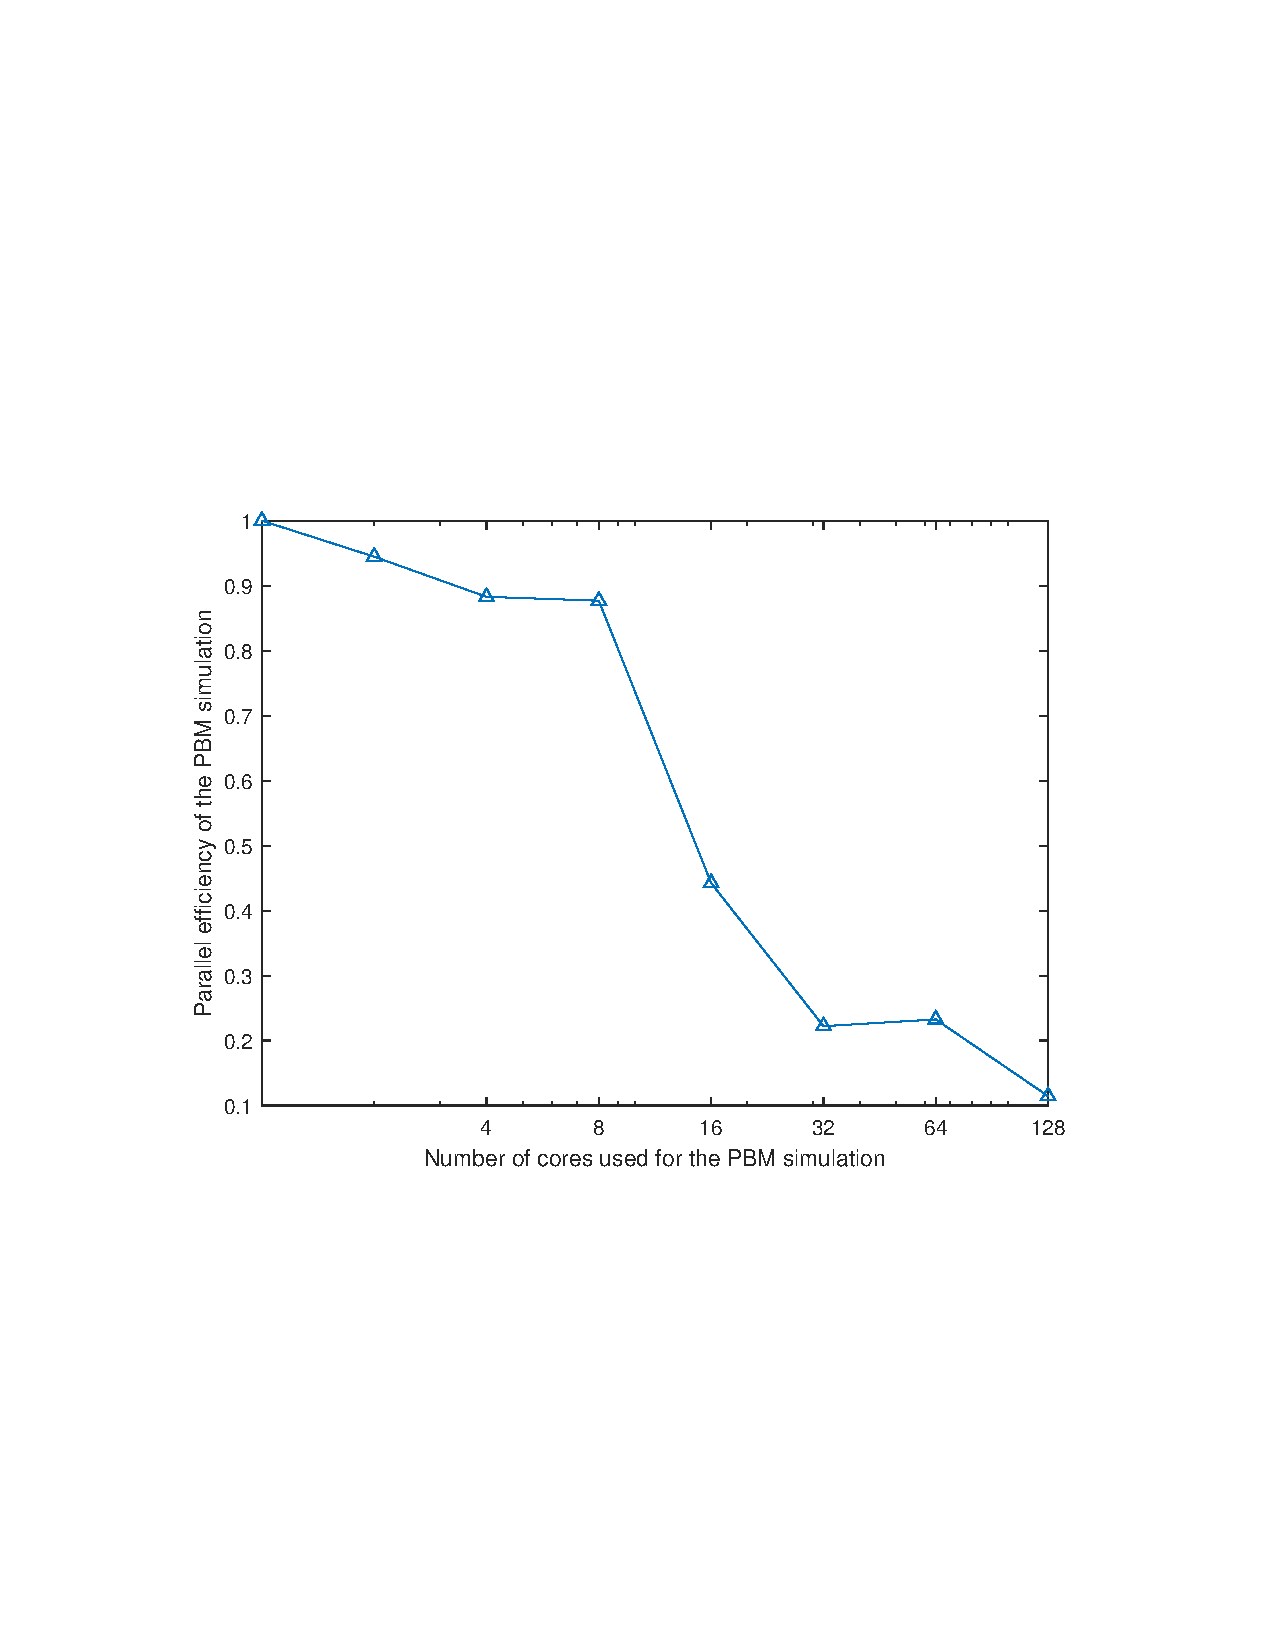
\includegraphics[scale=0.55]{rslsts_PBM_efficiency.pdf}
\caption{}
\label{fig:rslts_PBM_parallel_efficiency}
\end{subfigure}

\caption{\jhanote{please use consistent style in presenting the figures. The range of x-axis is the same but why use different major/minor points. this includes figure 9. Also shouldn't the y-axis of figure 10a also use multipliers of 2 for ease of readability?}(a) 
The speedup achieved by the hybrid parallel implementation of the PBM program.
It can be seen the initial speedup up to 16 cores as expected as from an ideal
parallel program where as it becomes almost constant from 32 cores to 128
cores(b) The parallel efficiency for the hybrid parallelized PBM code. The
efficiency of the code decreased as the number of cores are increased. The
higher number of cores have very low efficiency of about 11\% which depicted
that there is large time being spent in communication in between the cores.}
\end{figure}     

A similar behavior as Figure~\ref{fig:rslts_PBM_parallel_efficiency} was observed where the parallel 
efficiency of the program was plotted against the number of the cores used. This efficiency 
decreased as the number of cores used increased. The decrease in efficiency initially up till 8 cores 
was steep as the communication time in between the MPI process decreased the efficiency, deviating 
its value from the ideal of 1 to about 0.4. The implementation of OMP decreased the efficiency further 
as there was no major increase in the performance when compared to the increase in the number 
of cores used. The efficiency fell to as low as 11\% when 128 cores are used. 
Thus, there is scope for improvement in the parallel implementation 
of the program using OMP, especially in section of the code where nested loops are present.


\subsection{Coupled DEM and PBM physics}
The micro-scale simulations provide an insight about the physics of the system usually by tracking 
each particle. This micro-scale simulation data is useful for the development of macro-scale 
mechanistic models which take into account the dynamics of bulk of the particles and not individual 
particles. A similar approach has been implemented in this work, where a mechanistic aggregation 
kernel was developed from the DEM particle-particle collisions. Thus, the aim of this section was to 
illustrate that the physics of the system does not change to a great extent with the change in the size 
of the particles or the distribution of the particles.

Two simulations from the study were compared, the Coupled DEM and PBM simulation of the 2mm 
mono-sized particle and the second being the simulation where the inserted particles were in a size 
distribution. The ratio of rate of formation to the rate of depletion, both due to aggregation 
observed during these simulations was 0.5 which indicated that the both PBMs were stable.

One of the metrics to determine the physics of the system after a PBM simulation is to check the 
median diameter (D\textsubscript{50}) plots of the system after the granulation process. 
D\textsubscript{50} indicates the maximum diameter of particles that constitute 50\% of the total mass. 
These diameters vary along the length of the granulator since the granulated particles take time to 
pass through the granulator and that there is not enough liquid content in the later sections of 
the granulator to encourage the formation of granules. Thus, the D\textsubscript{50} for compartments 
in the latter section of the granulator is usually low. Figures~\ref{fig:rslts_PBM_2mm_d50} \& 
\ref{fig:rslts_PBM_psd_d50} show the D\textsubscript{50} plots of the mono-sized and PSD respectively. 
It can be seen that both these plots have a similar behavior when it comes to the nature of the 
increase of the D\textsubscript{50} during the granulation process. There is a difference of about 
20\% in the final diameter of the particles predicted, which at the of micrometer scale does not affect 
the final product quality. This slight deviation was observed due to the sudden jump in the 
rate of the aggregation which increased when particles from one compartment with higher 
D\textsubscript{50} got transferred to the next compartment with a lower D\textsubscript{50}. 
It can be seen from Figure~\ref{fig:rslts_DEM_timing_studies} that the 2mm mono-sized particle had a speed
advantage over the PSD simulation as it took about 1.6 times less. Since the physics of both the 
systems were not different, using the mono-sized simulations for the DEM could help save time on 
the overall simulations. 

\begin{figure}
\begin{subfigure}{.45\textwidth}
\centering
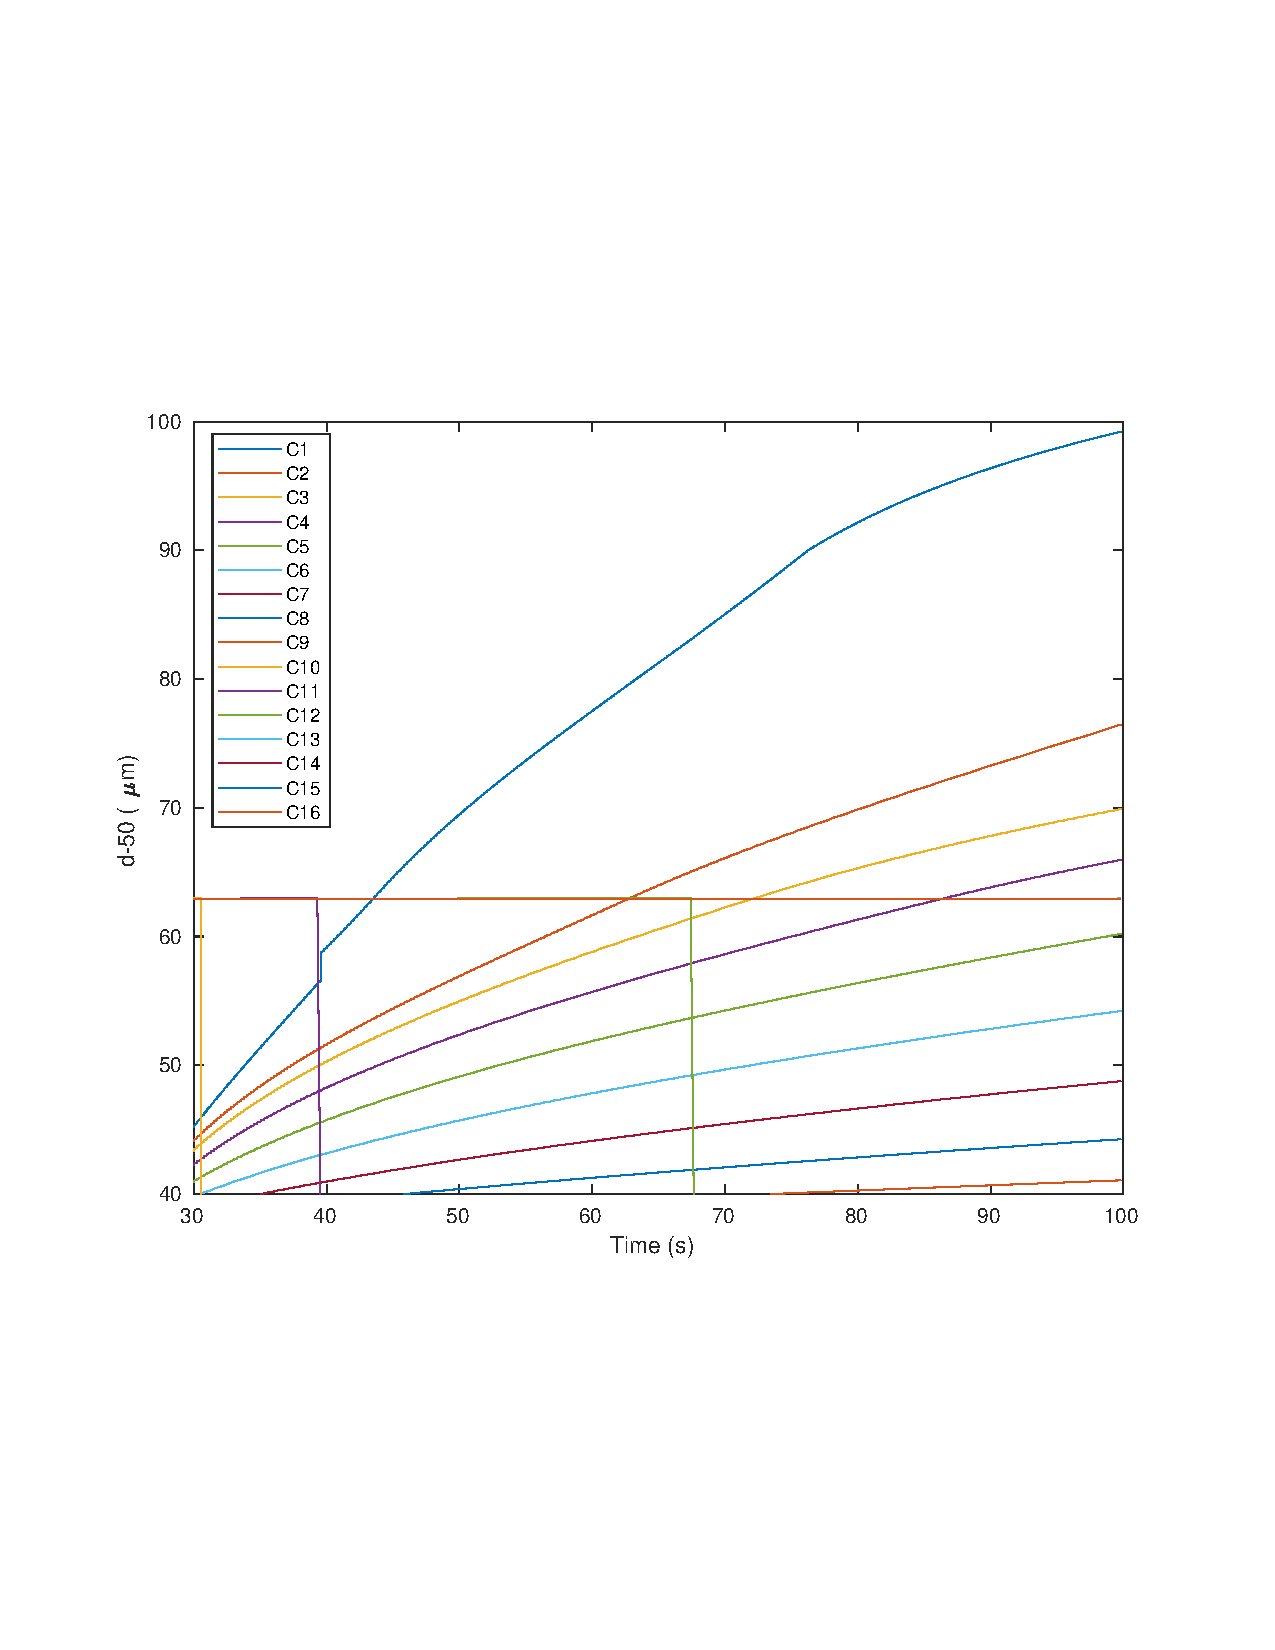
\includegraphics[scale=0.49]{rslts_pbm_d50_128_200.pdf}
\caption{}
\label{fig:rslts_PBM_2mm_d50}
\end{subfigure}\hfill
\begin{subfigure}{.45\textwidth}
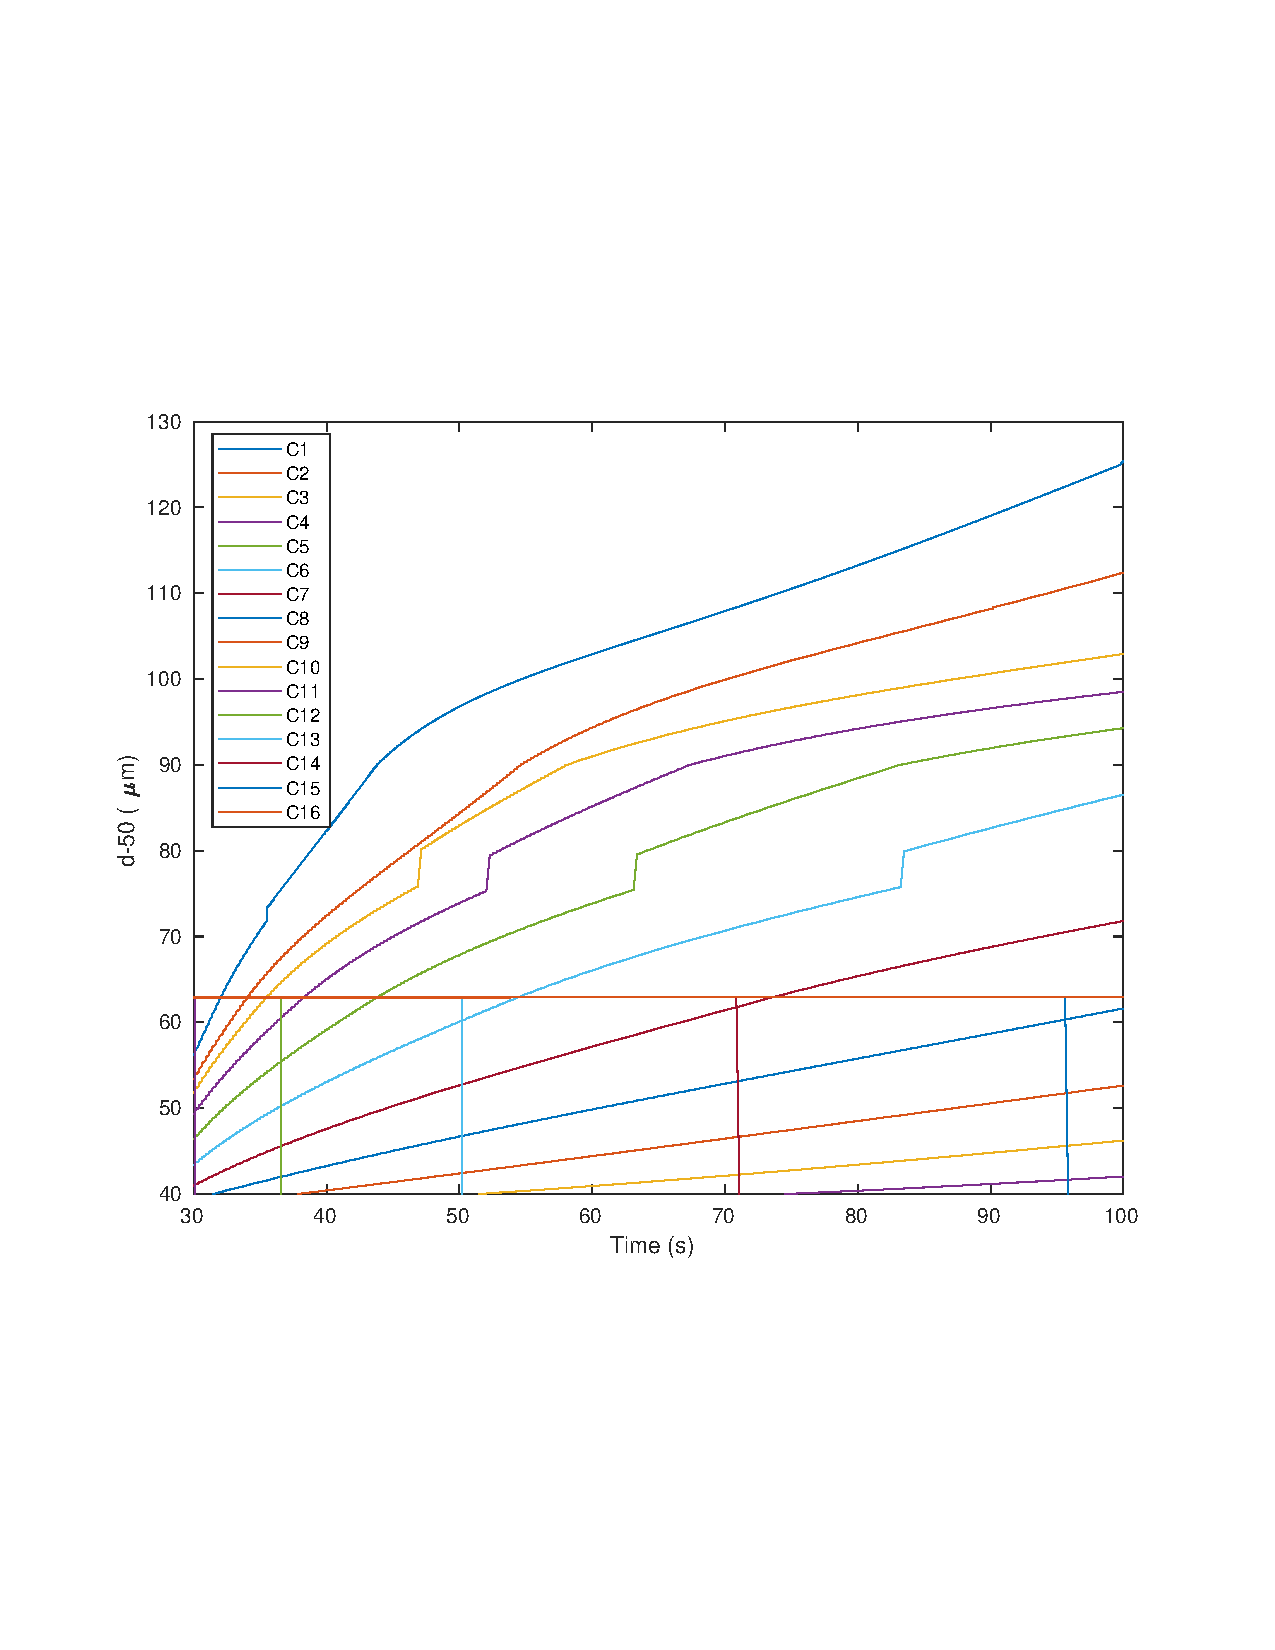
\includegraphics[scale=0.5]{rslts_pbm_d50_128_555.pdf}
\caption{}
\label{fig:rslts_PBM_psd_d50}
\end{subfigure}
\caption{(a) D\textsubscript{50} of the particles obtained after 100s of granulation time (25s of 
mixing and 75s of liquid addition) for the 2mm mono-sized particle DEM simulation. (b) D\textsubscript{50} of the particles obtained after 100s of granulation time (25s of mixing and 75s of liquid addition) for the distributed particle size DEM simulation. The trend observed was similar to the trend 
found in Figure \ref{fig:rslts_PBM_2mm_d50}. \jhanote{If you are putting two figures side by side and trying to compare, generally good to set the y-axis scale the same.} \jhanote{Figure description/caption should be self-contained to the extent possible.}}
\end{figure}  


\subsection{One-way coupled DEM+PBM using RADICAL-Pilot and its performance} 

\gpnote{This is said before. It can be removed:RADICAL-Pilot (RP) being a pilot job system it can bypass the need of
waiting on the long scheduler queues on a cluster for each individual task.} \jhanote{This is wrong! It
avoids the individual tasks from waiting for different periods of time at the
scheduler, not waiting itself at the scheduler!} \csnote{corrected, could you please check if it is clear now} 

\jhanote{consistency between
"the pilot", "pilot-job" and "RADICAL-pilot". "pilot" is a specific component; pilot-job is a  concept and concept, and "RADICAL-Pilot" is the software system. should not be used inter-changably. Also consistency between RP and other terms.} 

With resources allocated, the pilot can execute multiple simulations
\jhanote{what is a "simulation run" ? (as opposed to "simulations"?)} \\csnote(changed) 
at once.
The pilot job initiated the DEM simulation using the LIGGGHTS executable
compiled for the DEM studies and then created a link between the collision
data obtained, which was utilized by the PBM executable. After the link is
established, it also initiated the PBM. The timing profiles and results from
both the simulations were then obtained. Since the executables and inputs
files used in the simulations and the RP job \jhanote{now using RP job? what
is that?} were similar, we did not expect to see any changes in the physics of
the system. A value of 0.5 was obtained for the ratio of the rate of formation
to the rate of depletion due to aggregation.

\jhanote{Giannis: this paragraph is too long and unweildy. needs to be broken and rewritten.}
Since the platforms used for initial development and testing of the DEM and
PBM respectively were different, the DEM simulations were executed again on
Stampede2 for a fair and accurate comparison. The need for re-running the
simulations arises due to the clock speeds of the nodes and their
configuration for the 2 platforms were different. RADICAL-pilot was setup
for Stampede2 and aforementioned experiments were replicated. The DEM
simulations were run for 64, 128 and 256 cores (MPI processes) and the PBM was
run for 1, 2, 4, 8 and 16 MPI processes. No OMP threads were implemented for
the PBM run, since the current version of RP did not support threading. The
times for the individual DEM and PBM simulations were added to determine the
total amount time taken to simulate the one-way coupling. This time did not
include the time spent by each executable in the queue of the scheduler. This
time could vary from a few hours to a few days depending upon the load of the
cluster. The total time taken for the simulation using the RADICAL-pilot was
determined from the time the first DEM unit was executed until the PBM
execution completed. The time of the individual DEM and PBM simulation was
added to get the total amount of time it required for a single one-way
coupling simulation. Figure~\ref{fig:rslts_RP_time_plot} shows a comparison of
the total times of simulation in seconds for the sum of DEM and PBM individual
simulations to the times taken to run the simulations using RP. RP's
coordination layer tends to lose connection with the database when the
simulation time exceeds 6 hours. In order to address this issue, the DEM
simulations had to be restarted after $1~second$ of simulation, which led to
an increase in the simulation times of the DEM. This can be observed in
Figure~\ref{fig:rslts_RP_time_plot}. There is also a small time penalty that
is paid for the communication in between the client and resource as RP needs
to link the required files for the next simulation and also determine the
state of the simulation.
 \gpnote{Do you agree with the following statement:
In addition, we had to partition DEM execution to smaller parts, because RP coordination
layer was timing out after 6 hours of a single simulation.} \csnote{added the restart DEM part.}
 But, this communication time was significantly lower than the total
amount of time a executable job would spend in the job scheduler queue.
Thus, when a large number of these simulations need to be run, they could \jhanote{??} uploaded 
as a single pilot job using RADICAL pilot reducing scheduler wait times on individual 
jobs. \jhanote{It is unclear what the
benefit is!}\csnote{tried to address the benefit elaborately} 
An extension of this work would be to use RP to schedule multiple such coupled simulations 
as one job, thus decreasing the wait times even further.
\begin{figure}
\centering
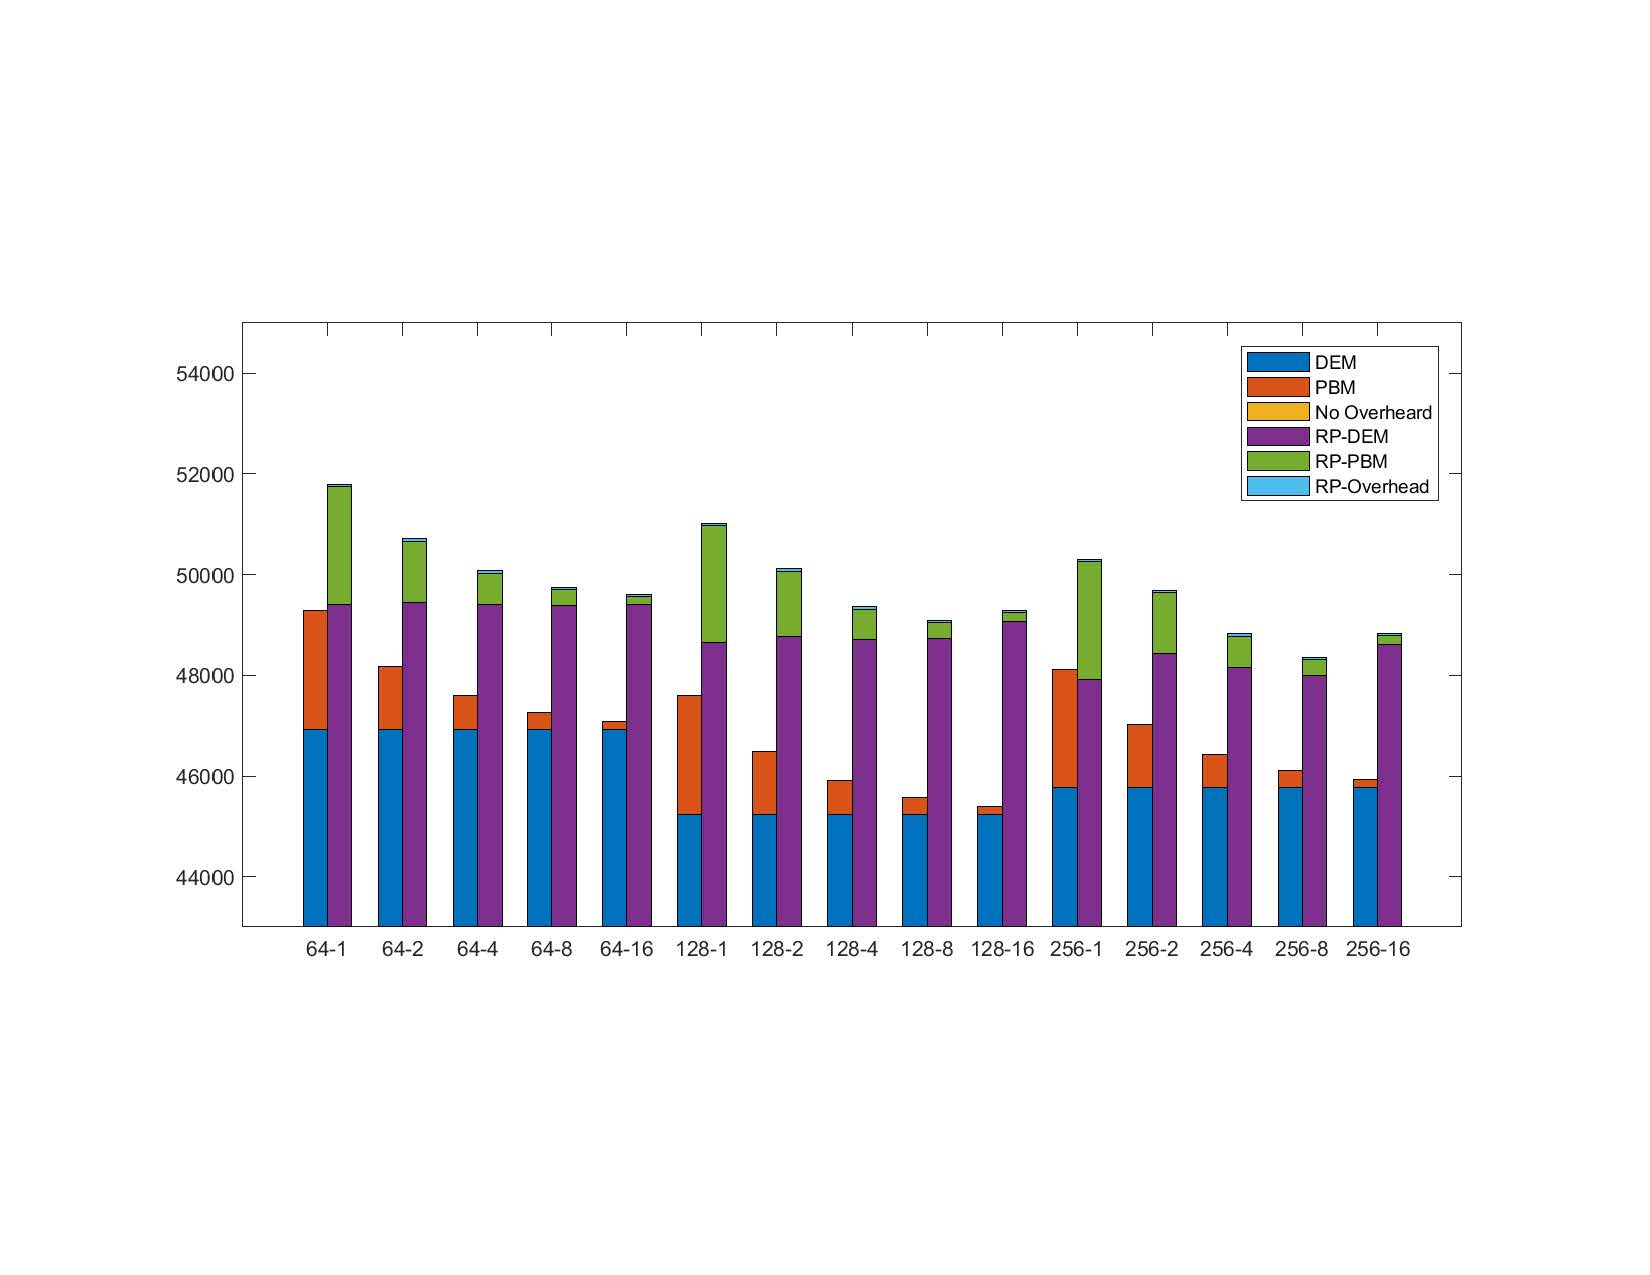
\includegraphics[scale=0.7]{rp_final.pdf}
\caption{\jhanote{y-axis unit is missing} \jhanote{"overheard" --> "overhead"} A comparison of times taken by 2 individual simulations (DEM and PBM) (without 
including queue time) to the  time taken by each simulation in the pilot job
of the Radical-Pilot. \jhanote{Giannis: Radical-Pilot --> RADICAL-Pilot. But
more importantly, "pilot job" of the RADICAL-Pilot does not make sense.}
\jhanote{Giannis: (i)Overheads do not show up any where? (ii) "64-1", "62-2"
is not obvious to reader.}A small communication time overhead can be seen
which is a very small when compared to the time of the complete simulation.}
\label{fig:rslts_RP_time_plot}
\end{figure}
	    
\section{Conclusions}
A simple uni-directional DEM+PBM coupled study for a high shear granulator has been 
presented. DEM simulations were used to determine the movement of the particles inside 
the granulator and to obtain the collision data. This collision data was then used in 
the multi-dimensional PBM which was developed with 2 solid bins. Both these executables 
were parallelized to help them utilize the multi-core hardware of a cluster. The DEM 
was parallelized using MPI where as the developed PBM used MPI as well as OMP for a 
faster execution. The speed-up achieved for the DEM simulation was about 12 times using 
64 cores, where as the PBM achieved a speed-up of 14 times when 16 cores were used. 
RP was utilized to execute the simulations for lower wait times. A more accurate 
model for the high shear granulator would be to couple the DEM and PBM bidirectionally 
i.e. these two methods are executed iteratively up till a steady state is reached. 
For the two-way coupling, the computation resources required would be really large 
as it would involve multiple DEM and PBM simulations. The role RP in such a 
detailed simulation would be more crucial as it would need to handle more 
communications and various job submissions. This would also help reduce 
total time taken to complete the required runs.

\section*{Software and Data}
\noindent Source code and input scripts \jhanote{what is the difference between input and analysis scripts?} for reproduction of the experiments can be found at:\\
Cybermanufacturing: \url{https://github.com/radical-collaboration/CyberManufacturing}
\jhanote{I was not able to find "input scripts" to reproduce experiments. I
would create a README at the github with links to the source code (for what?)
etc} 
\csnote{input files for ligghts are in dir src\/liggghts\_input\_files and the execution details are already on Wiki}


\section*{Acknowledgments}
\noindent The authors would like to acknowledge National Science Foundation (NSF) for 
funding this project through the grant number: 1547171. Computational resources 
were provided by NSF XRAC award TG-MCB090174.


\appendix
%\section{PBM Parallelization}
%\label{app:parallelPBM}
%The parallelization technique used for the PBM used was dependent on the number of 
%compartments present inside granulator. Each of the compartments, had calculations 
%independent from each other for each time step. So each of them were loaded 
%onto different MPI processes. Since there is minimal communication between them, 
%they could easily be parallelized using MPI. To get further speed improvements, 
%the time independent calculations of the PBM were parallelized using OMP. This 
%parallelization technique is decried as an algorithm in Algorithm \ref{alg:parpbm}.
%
%OMP was used to parallelize the calculations inside each compartment. Since 
%the PBM consisted of 2 solid bins, one of the solid bins was parallelized. 
%The number of solid bins of solid were equally divided by the number of OMP threads. 
%%Figure~\ref{fig:app_OMP_distribution} depicts the equal distribution of 16 solid bins of the second solid using 4 OMP 
%%threads.

     

 
%\begin{figure}[H]
%\centering
%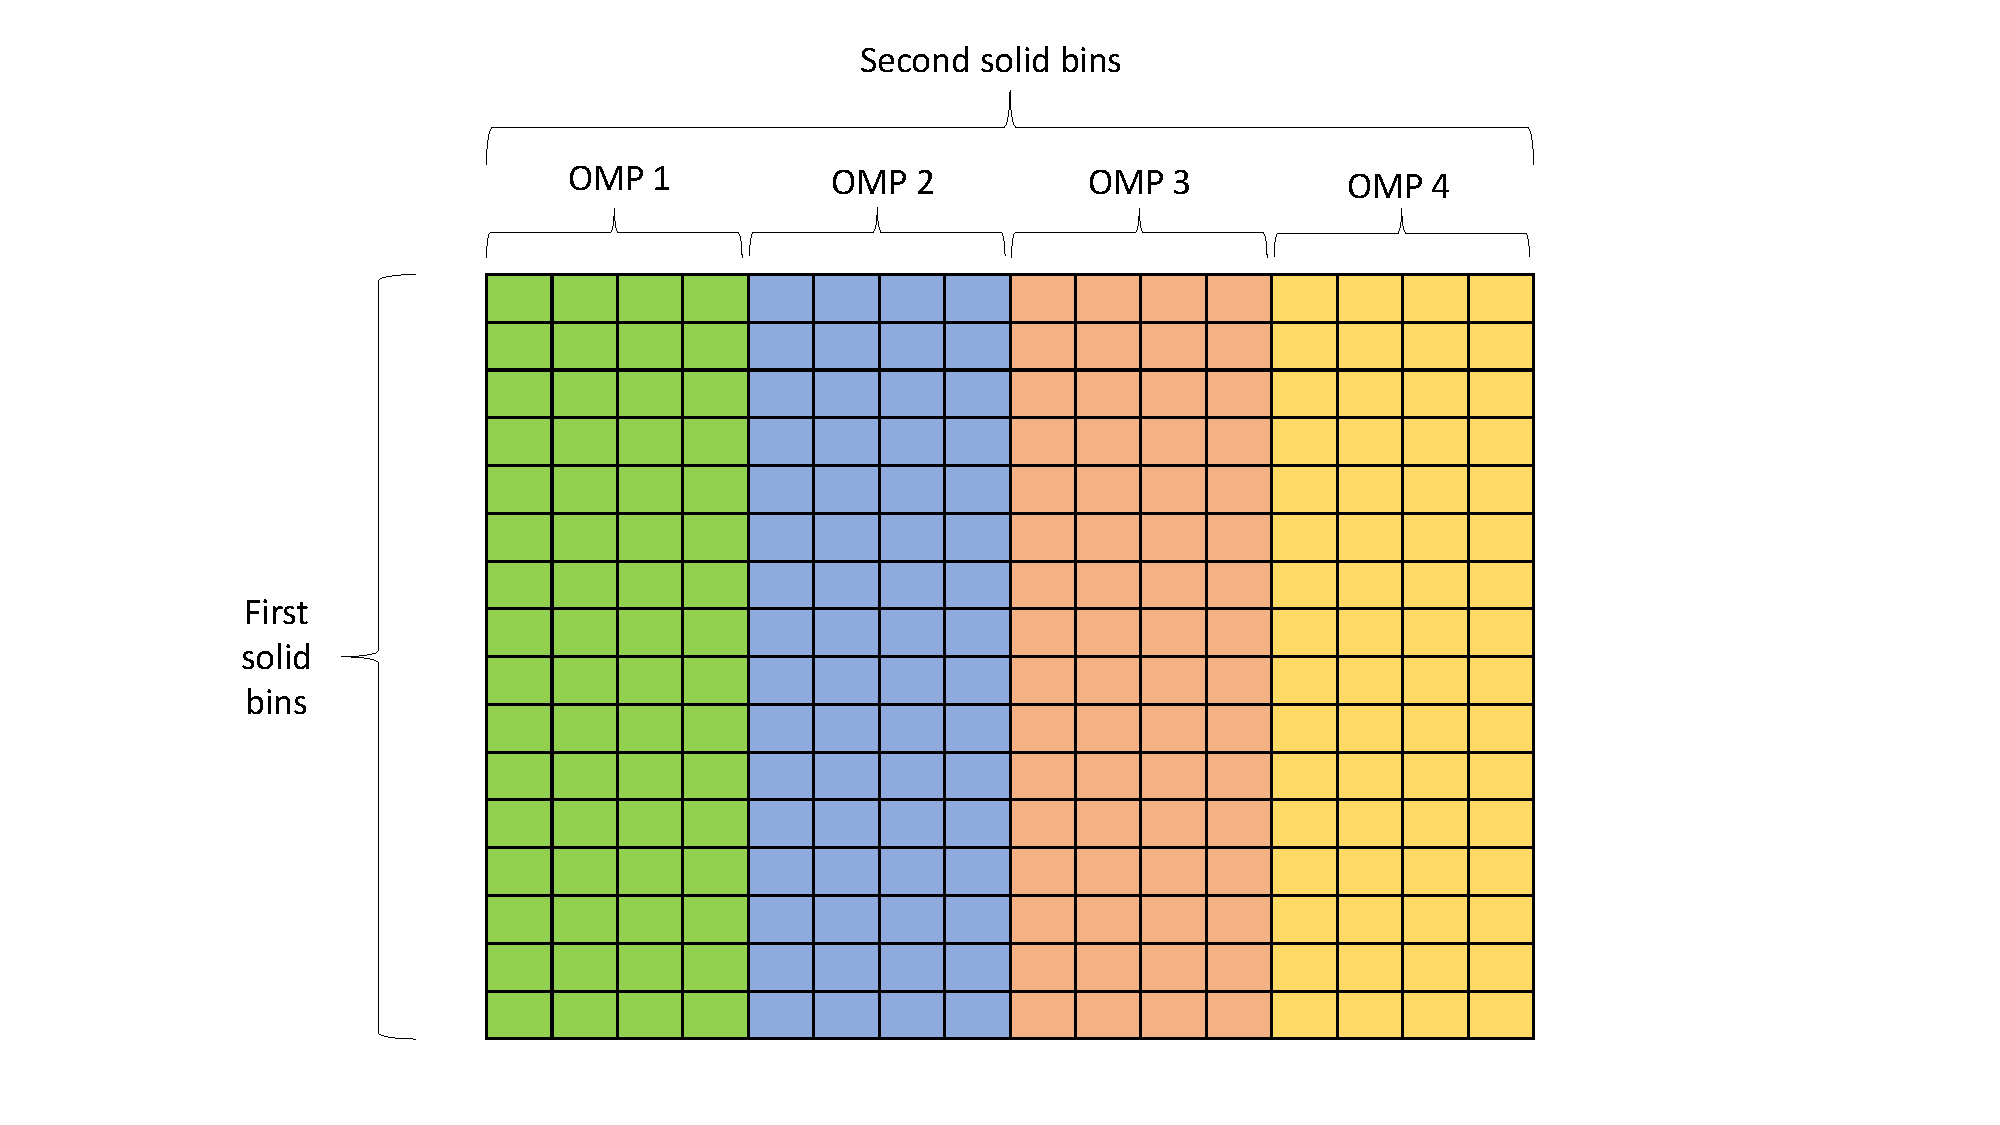
\includegraphics[scale=0.5]{OMP_table.pdf}
%\caption{The integration of aggregation rate distributed among OMP processes. This figure indicates the use of 4 OMP processes, the 
%configuration that gave us the best performance. This technique has been implemented for each MPI process.}
%\label{fig:app_OMP_distribution}
%\end{figure}	

\section*{References} 
\bibliographystyle{elsarticle-harv}
\bibliography{Bibli}
\end{document}